\documentclass{article}      % Specifies the document class
\usepackage{graphicx}		 % Need this to include images
\usepackage[hyphens]{url}
\usepackage[hidelinks]{hyperref}
\usepackage{multirow}
\usepackage{array}
\usepackage{parskip}
\usepackage[acronym]{glossaries}
\usepackage{ngerman}
\usepackage{textcomp}
\usepackage{listings}
\usepackage{xcolor}
\usepackage{amsmath}
\usepackage{caption}
\usepackage{subcaption}
\usepackage{makecell}
\usepackage[toc,page]{appendix}

\selectlanguage{english}
\usepackage[utf8]{inputenc}

% Add another layer to the Index
\setcounter{tocdepth}{4}
\setcounter{secnumdepth}{4}
 
\lstdefinestyle{mystyle}{
    backgroundcolor=\color{backcolour},   
    commentstyle=\color{codegreen},
    keywordstyle=\color{magenta},
    numberstyle=\tiny\color{codegray},
    stringstyle=\color{codepurple},
    basicstyle=\ttfamily\footnotesize,
    breakatwhitespace=false,         
    breaklines=true,                 
    captionpos=b,                    
    keepspaces=true,                 
    numbers=left,                    
    numbersep=5pt,                  
    showspaces=false,                
    showstringspaces=false,
    showtabs=false,                  
    tabsize=2
}

\renewcommand\theadalign{bc}
\renewcommand\theadfont{\bfseries}
\renewcommand\theadgape{\Gape[4pt]}
\renewcommand\cellgape{\Gape[4pt]}
 
\lstset{style=mystyle}

\makeglossaries
 
\newacronym{api}{API}{Application Programming Interface}
\newacronym{asi}{ASI}{Automatic Subject Indexing}
\newacronym{asl}{ASL}{Asymmetric Loss}
\newacronym{aml}{AML}{Asymmetric Max-constraint Loss}
\newacronym{bce}{BCE}{Binary Cross Entropy}
\newacronym{cli}{CLI}{Command-Line Interface}
\newacronym{cbow}{CBOW}{Continuous-bag-of-words}
\newacronym{cnn}{CNN}{Convolutional Neural Network}
\newacronym{cpu}{CPU}{Central Processing Unit}
\newacronym{csv}{CSV}{comma-separated values}
\newacronym{ddc}{DDC}{Dewey Decimal Classification}
\newacronym{ert}{ERT}{Extended Representing Text}
\newacronym{fnn}{FNN}{Feed-forward Neural Network}
\newacronym{fl}{FL}{Focal Loss}
\newacronym{fu}{FU}{Free University}
\newacronym{gb}{GB}{Gigabytes}
\newacronym{gflops}{GFLOPS}{Giga- Floating Point Operations Per Second}
\newacronym{hlse}{HLSE}{Hierarchical Label Set Expansion}
\newacronym{hmc}{HMC}{Hierarchical Multi-label Classification}
\newacronym{hu}{HU}{Humboldt University}
\newacronym{http}{HTTP}{HyperText Transfer Protocol}
\newacronym{json}{JSON}{JavaScript Object Notation}
\newacronym{kg}{KG}{Knowledge Graph}
\newacronym{kge}{KGE}{Knowledge Graph Embedding}
\newacronym{kos}{KOS}{Knowledge Organization System}
\newacronym{lca}{LCA}{Lowest Common Ancestor}
\newacronym{lcas}{LCAS}{Lowest Common Ancestor Score}
\newacronym{lda}{LDA}{Latent Dirichlet Allocation}
\newacronym{ml}{ML}{Machine Learning}
\newacronym{mcl}{MCL}{Max-constraint Loss}
\newacronym{mcm}{MCM}{Max-constraint Module}
\newacronym{mag}{MAG}{Microsoft Academic Graph}
\newacronym{makg}{MAKG}{Microsoft Academic Knowledge Graph}
\newacronym{mb}{MB}{Megabytes}
\newacronym{mlc}{MLC}{Multi-label Classification}
\newacronym{mlp}{MLP}{Multi-layer Perceptron}
\newacronym{nlp}{NLP}{Natural Language Processing}
\newacronym{oaipmh}{OAI-PMH}{Open Archives Initiative Protocol for Metadata Harvesting}
\newacronym{pos}{POS}{Part-of-speech}
\newacronym{ram}{RAM}{Random Access Memory}
\newacronym{rnn}{RNN}{Recurrent Neural Network}
\newacronym{rds}{RDS}{Relational Database Service}
\newacronym{rdf}{RDF}{Resource Description Framework}
\newacronym{srt}{SRT}{Simple Representing Text}
\newacronym{sota}{SOTA}{State-of-the-art}
\newacronym{sgd}{SGD}{Stochastic Gradient Descent}
\newacronym{si}{SI}{Subject Indexing}
\newacronym{sm}{SM}{Supervised method}
\newacronym{tu}{TU}{Technical University}
\newacronym{umls}{UMLS}{Unified Medical Language System}
\newacronym{um}{UM}{Unsupervised method}
\newacronym{vm}{VM}{Virtual Machine}
\newacronym{xmc}{XMC}{Extreme Multi-label Classification}

\makeatletter
\newcommand\HUGE{\@setfontsize\Huge{50}{60}}
\makeatother

\DeclareMathOperator*{\argmax}{arg\,max}
 
\begin{document}

%title page
\thispagestyle{empty}
\begin{center}
\begin{minipage}{0.9\linewidth}
\centering
	      		 
	%University logo
    
\includegraphics[width=0.5\linewidth]{figures/tub.jpg}
    \vspace{1cm}

    % Title
	{\scshape{\HUGE Master Thesis Draft\par}}
	\vspace{1cm}
	%Thesis title
    {\scshape{\Large subject indexing for institutional repositories\par}}
    \vspace{1.5cm}
  
 Author  \linebreak
 {\Large Mohamed Mesto \par}
 	\vspace{1.5cm}

\flushleft

\begin{tabular}{ll}
Berlin, 2022 \linebreak
\vspace{1cm}&   \\
  University ID: & 390*** \vspace{0.3cm} \\ 
  Course: & Computer Science \vspace{0.3cm} \\
  First Referee: & Prof. Dr. Manfred Hauswirth \vspace{0.3cm} \\
  Second Referee: & Prof. Dr. Volker Markl \vspace{0.3cm} \\
  Supervisor: & Dr. Sonja Schimmler \\
 \end{tabular}

\end{minipage}
\end{center}
\clearpage

\pagebreak

\tableofcontents \pagebreak

\listoffigures \pagebreak

\listoftables \pagebreak
 
\printglossary[type=\acronymtype, style=super,  nonumberlist, nogroupskip] \pagebreak

\begin{center}
  \textbf{DECLARATION OF AUTHENTICITY}
\end{center}
I, Carlos Franzreb, declare that I wrote this thesis independently and did not use any unnamed sources or aid. To the best of my knowledge, this thesis contains no material previously published, except where due reference is made by correct citation.

\vskip 2cm

Berlin, 10.03.2021 \pagebreak
\begin{abstract}
This thesis evaluates the performance of supervised and unsupervised methods for performing subject indexing on institutional repositories, which are small and multidisciplinary. Our unsupervised approach is inspired by the \acrfull{mag}, where the documents and subjects are vectorized and compared in vector space. For the supervised approach, we implement a convolutional neural network and train it on a set of \acrshort{mag}'s indexed documents. The two methods are evaluated with data extracted from the repositories of Berlin's three universities, which show that the supervised approach is more accurate. Its design enables it to be used in other repositories without any modifications.
\end{abstract}

\vspace{1cm}

\selectlanguage{ngerman}
\begin{abstract}
In dieser Arbeit wird die Leistung von überwachten und unüberwachten Methoden für die thematische Indexierung von kleinen und multidisziplinären institutionellen Repositorien bewertet. Unser unüberwachter Ansatz orientiert sich am \acrfull{mag}, bei dem die Dokumente und Themen vektorisiert und im Vektorraum verglichen werden. Für den überwachten Ansatz implementieren wir ein faltendes neuronales Netzwerk und trainieren es auf einer Reihe von indexierten Dokumenten des \acrshort{mag}. Die beiden Methoden werden mit Daten aus den Repositorien der drei Berliner Universitäten evaluiert. Daraus zeigt sich, dass der überwachte Ansatz genauer ist. Sein Design ermöglicht es, ihn ohne Änderungen in anderen Repositorien zu verwenden.
\end{abstract}
\selectlanguage{english} \pagebreak

\section{Introduction}

\acrfull{si} consists on assigning the appropriate subjects to each document of a collection. The subjects describe the content of the document, and can be used to relate documents to one another. Large collections of documents are often hard to navigate, which is why metadata, including subjects, is important. They make the information in the collection more accessible.

Institutional repositories are databases that public institutions, such as universities, use to store and index the outputs of their research \cite{barton2004creating}. Such repositories profit from having a thorough set of subjects that provides structure to its content. Therefore, in this thesis we explore the problem of extending institutional repositories with \acrshort{si}. We focus on repositories that are small and multidisciplinary. By small, we don't refer to hundreds of documents, but rather tens of thousands, which is considered small in the era of big data and deep learning.

We have constructed a dataset for our experiments with the repositories of Berlin's three universities: the \acrfull{tu}, the \acrfull{hu} and the \acrfull{fu}. They all have institutional repositories, called depositonce, edoc and refubium, respectively. The medical university, called Charité, also uses refubium to post their work online. All three repositories offer their data through the Open Archives Initiative Protocol for Metadata Harvesting (OAI-PMH)\footnote{\url{https://www.openarchives.org/pmh/}}.

These repositories already have subjects, but they are of little use. Over 80 \% of them appear only once and therefore cannot be used to relate documents. Furthermore, the subjects are different in each repository. This hinders their interoperability, which is one of the goals of public repositories \cite{barton2004creating}. This thesis aims to increase the quality of the \acrshort{si} and to standardize it in such a way that documents from different repositories can be related to one another.

The easiest way of introducing high quality subjects in different repositories is using an external source. We retrieve 2,157 subjects from the \acrfull{mag} \cite{shen2018web}, evenly spread across its 19 fields of study. This subset covers broad topics of numerous disciplines, such as \textit{Physics} and \textit{Philosophy}, which makes it ideal for our multidisciplinary dataset. We focus specifically on machine learning approaches, implementing methods of the two larger paradigms: supervised and unsupervised approaches.

Our unsupervised approach closely follows the \acrshort{si} procedure of \acrshort{mag}. The \acrshort{mag} also handles multidisciplinary data and is, to the best of our knowledge, the most successful unsupervised method for \acrshort{si}, with an accuracy of 80 \%. Documents are enriched with data from their venues, advisors and referees, whereas subjects are represented with text from their corresponding Wikipedia articles. Then, all these representations are vectorized using word embeddings trained with the skip-gram model \cite{mikolov2013distributed}. Subjects are finally assigned to documents by evaluating their similarity in vector space.

Our supervised approach consists of a convolutional neural network, which we train with over 200,000 scientific texts from \acrshort{mag} that are assigned the subjects of our subset. The model learns to assign subjects to documents on a larger dataset, and is then applied to the documents from the repositories. Our model comes from a similar use case \cite{gargiulo2019deep}, where the subjects also form a hierarchy and are assigned to scientific documents.

We extend the model in two different ways. We first address the asymmetry that arises from documents being assigned only a few from many subjects, and then by ensuring that the outputs of the model don't violate the subject hierarchy. The three resulting models have only minimal differences, but they still yield different results in our evaluation sets. The original model performed best.

The best supervised model is then compared with the unsupervised approach on three evaluation sets that we have extracted from the repositories. Two of these sets consider only the 19 fields of study, covering more than 70 \% of all documents. The other set considers all 2,157 subjects. It covers 24 \% of the documents, with mostly one subject assigned to each document.

There are numerous metrics used in \acrshort{si}. Many of them can be adapted to consider the subject hierarchy, which introduces relationships among the concepts. The evaluation of a subject-document pair is not binary anymore, as certain pairs are better than others when considering the distance of the guess to the correct subjects in the hierarchy. Our evaluation set differs from the common scenario in its sparsity: documents appear mostly once in each evaluation set, meaning that we don't have the full set of subjects for the documents. We consider this when designing our evaluation metrics, which comprise a flat metric and a hierarchical one.

Our experiments show that the supervised method is significantly more accurate. We therefore conclude that supervised approaches are better suited for \acrshort{si} tasks in small and multidisciplinary repositories. They also have the most potential and, considering our two approaches, they are easier to implement.

\subsection{Outline}

The following chapters are structured as followed. Chapter \ref{problem} starts with the introduction of the problem tackled by this thesis. We then present its scope, defining which types of documents we index, and which \acrshort{si} methods we consider. We also present the 2,157 \acrshort{mag} subjects that we will use to index the documents. Finally, we present our objectives by formulating a research question.

We then perform an analysis of the institutional repositories of the three Berlin Universities in chapter \ref{repo_analysis}. We evaluate the existing subjects of the repositories, concluding that most of them cannot be used to relate documents to one another. We explore venues, advisors and referees, as these will be used to relate documents in the unsupervised approach. We finally assess the quality of the data, finding that 6 \% of the documents don't have an abstract and many others have abstracts in languages other than English.

Chapters \ref{subject_indexing} and \ref{hmc} present the literature on unsupervised and supervised approaches, respectively. Chapter \ref{subject_indexing} also presents several ways of classifying \acrshort{si} methods. They mainly consider the existence of a set of subjects and the availability of training data. Chapter \ref{hmc} presents the work on \acrfull{hmc}, where objects assigned a variable number of labels, and the labels are structured as a hierarchy. Objects may be images, proteins or, as in our case, text. \acrshort{si} is an application of this problem. This chapter presents the common ways of tackling this classification problem, as well as several implementations.

Our unsupervised approach is presented in chapter \ref{unsupervised_approach}, whereas the supervised approach is outlined in chapter \ref{supervised_approach}. Both were already introduced above. The supervised and unsupervised approaches are compared in chapter \ref{eval}, where our three evaluation sets and two metrics are also presented. We end this thesis with chapter \ref{conclusion}, where we discuss the differences between the approaches regarding their performance, implementation and interpretability. We also define the applicability of the supervised approach, which performs best.
\section{Problem definition} \label{problem}

In this chapter, we introduce the problem this thesis addresses and define the scope of our work. We also formalize the problem by formulating a research question, and present the approaches we will implement.

The problem, presented in section \ref{problem_intro}, arises from the poor quality of the subjects that are currently present in the repositories. 81 \% of all subjects are only assigned to one document, and only 5 \% of the subjects are assigned to more than three documents. This makes it hard to navigate the repositories by filtering the documents by subject, which is the purpose of having subjects. The sets of subjects are also different for each repository, which hinders the interoperability.

In section \ref{problem_scope} we define the scope of this thesis. We only consider the titles and abstracts of theses and publications written in English, which reduces the complexity of the task without hindering its research interest. We also restrict ourselves to evaluating methods that use an existing set of subjects. We use the subjects extracted from  the \acrfull{mag}, which is able to identify the relevant concepts in science because of its size. These subjects can then be used for any multidisciplinary repository, other than those included in our experiments.

Once the problem and scope have been introduced, we formalize the problem by formulating the research question this thesis attempts to answer, in section \ref{problem_rq}. This thesis focuses on the evaluation of supervised and unsupervised algorithms for performing \acrlong{si} in small and multidisciplinary repositories. 

\subsection{Introduction} \label{problem_intro}

As discussed in chapter \ref{repo_analysis}, the subjects that are currently present in the repositories are not well maintained. 81 \% of all subjects occur only once, i.e. they are only used by one publication. These cannot be used to relate documents. Furthermore, only 5 \% of the subjects are used by more than 3 publications. The poor quality of the subjects decreases the accessibility of the repositories. Each of them contains thousands of documents, and navigating them can be a cumbersome task. Subjects can be a useful tool for finding the desired documents, and also for looking for documents that are related to the ones we are currently reading.

Consider a repository where there is a maintained set of subjects. Each document in the repository is assigned a subset of these subjects, which can be navigated through the document's page in the repository. If a user is currently reading a publication about brain-computer interfacing, and would like to read more about that topic, the user could browse other documents that handle it by clicking on the corresponding subject. Furthermore, if the user has trouble understanding one of the building blocks of the documents, the user can click on the corresponding subject to search for other documents that maybe present that concept in more detail.
\subsection{Scope} \label{problem_scope}

Thus, our goal is to improve the quality of the \acrshort{si} in the repositories. In this section, we define the scope of this thesis. We do so before formulating the research question, as if not the problem is too broad and unclear.

Performing subject indexing in all the documents would require a lot of software engineering and special treatment of certain types of documents. This would hinder the scientific purpose of this thesis. We therefore start by considering which documents should be indexed in section \ref{problem_scope_docs}. Those documents will form our dataset. Then, in section \ref{problem_scope_asi}, we discuss which type of indexing methods will be implemented and evaluated in this thesis. We pick one of the two main paradigms of subject indexing and argue why it is better suited to our use case. Our approaches require a set of subjects, which they will assign to the documents of our dataset. We define this set in section \ref{problem_scope_subjects}. We explain several choices we have made, such as its size and composition.

\subsubsection{Documents} \label{problem_scope_docs}

The scope of this work are the publications and theses written in English. In the repositories there are also data files and other types of documents, but they are not suited for this work because of their lack of text and variety in format. Which document types are included in the dataset are shown in table \ref{tab:document_types}.

Only English documents (and English metadata, for that matter) are considered because it greatly reduces the complexity of the task and doing so does not seem to reduce the quality of the data. For example, out of the 28,720 documents present in the Free University's repository, 21,701 of them have the same number of English subjects as they have German subjects. A probable cause of this is that ones are the translations of the others. If this were the case, discarding the German subjects would not imply information loss. Also, adding other languages to the \acrshort{si} pipeline would not introduce any major changes in how we assign subjects to documents. There is therefore no research interest in doing so.

Instead of using the full texts of each document, we will only use the titles and the abstracts. This should reduce the computational cost of our approaches and also facilitate the encoding task, as only the most important aspects covered by the paper are taken into account. Using the full texts could potentially reduce the quality of the encodings, as they cover more topics. Especially theses, which sometimes comprise hundreds of pages and are broad in their content, would be expensive to process and hard to index.

We also harvest further metadata from the documents, such as subjects, publication venues, as well as the advisors and referees of theses. All these are used to create evaluation datasets, as explained in section \ref{eval_datasets}, and all except the subjects are also part of the unsupervised approach.

\begin{table}
\begin{center}
 \begin{tabular}{| c | c | c|} 
 \hline
 \thead{Kept?} & \thead{Group} & \thead{Types} \\ [0.5ex]
 \hline\hline
 \makecell{Yes} & \makecell{Thesis} & \makecell{Doctoral thesis, Bachelor thesis, Master \\ thesis, Study thesis, Habilitation} \\ 
 \hline
 \makecell{Yes} & \makecell{Publication} & \makecell{Preprint, Book part, Book, Article, \\ Conference proceedings, Conference \\ object, Periodical part, Working paper, \\ Research paper, Report} \\
 \hline
 \makecell{No} & \makecell{Data} & \makecell{Video, 3D Model, Textual data, Audio, \\ Sound, Moving image, Image, Dataset, \\ Generic research data, Research data} \\
 \hline
 \makecell{No} & \makecell{University} & \makecell{Course material, Lecture} \\
 \hline
 \makecell{No} & \makecell{Other} & \makecell{Draft, Software, Collection, Review, Other} \\
 \hline
\end{tabular}
\caption{All the document types present in the three repositories. The groups are only for clarity.}
\label{tab:document_types}
\end{center}
\end{table}
\subsubsection{Subject Indexing} \label{problem_scope_asi}

In chapter \ref{subject_indexing}, we discuss the different ways in which \acrshort{si} approaches can be classified. For now, we only require the distinction between \textit{assigned SI} and \textit{derived SI}, which differ on the subjects that are used to index the documents. In assigned \acrshort{si}, an existing set of subjects is used. The set can be constructed manually or retrieved from another application. On the other hand, derived \acrshort{si} extracts the subjects from the documents using only intrinsic information, such as term frequency.

Assigned \acrshort{si} is the preferred approach for information retrieval because it offers better precision and recall, given that users don't always know exactly the subjects they are looking for \cite{golub2019automatic}. Furthermore, using the same set of subjects in all three repositories allows them to be searched together. If each repository had its own set of subjects, their accessibility would be hindered. This is why standard sets of subjects, such as the \acrfull{ddc}, are so useful.

Given the heterogeneity and the technical nature of our dataset, derived \acrshort{si} approaches would not reach the desired quality. Our heterogeneous dataset limits the performance of term-weighting methods, such as TF-IDF, as phrases that are relevant because of their scientific meaning may not appear often enough to be noticed by these methods. Because of this, and given the availability of a suitable set of subjects, we will focus solely on methods that perform assigned \acrshort{si}. The existing subjects in the repositories will be used only for evaluation purposes.

We will use the subjects from \acrfull{mag}, a scientific knowledge graph presented in section \ref{subject_indexing_mag}. The set Microsoft has built covers all the disciplines present in the repositories and is therefore well suited for our task. It also includes a hierarchy, which we will use when training classification models. In the following section, we further discuss the \acrshort{mag} set of subjects. We argue why a subset of them suffices for our approach and which size and composition we require. We then present the final set of subject we use in this thesis.
\subsubsection{Set of subjects} \label{problem_scope_subjects}

Our dataset comprises considerably fewer documents than \acrshort{mag} (tens of thousands instead of hundreds of millions). Given that our goal is to relate documents to one another through their content, and we are focusing on small repositories, we don't require such granular subjects. If we used all the \acrshort{mag} subjects, most of them would be left unassigned, and many others would be assigned only once. We therefore pick a subset of these subjects.

\acrshort{mag} structures their set of subject as a hierarchy, where the first level comprises 19 subjects, which we call fields for clarity. Under each field, there exist five further hierarchy levels. We extract the subjects from OpenAlex, which is currently the best data source for subjects and publications of \acrshort{mag} (see section \ref{mag_access_data}).

In section \ref{problem_scope_subjects_retrieve}, we present our subject retrieval procedure. We discuss how many subjects we retrieve per field, and on what conditions we pick among the thousands of candidates. Then, we present the resulting set of subjects in section \ref{problem_scope_subjects_result}.

\paragraph{Subject retrieval} \mbox{} \label{problem_scope_subjects_retrieve}

We have extracted up to 200 descendants of each of the 19 fields. We consider how many publications a subject has been assigned to, assuming that popular subjects are more likely to appear in the repositories. We have tried different thresholds for how many assignments a subject needs to be considered, to strike a balance between picking subjects from the upper levels, which are more general, and picking subjects that are popular.

The problem is that the fields differ in popularity. For example, \textit{Medicine} has more than 200 subjects in the third level with more than 25k works, whereas \textit{Environmental science} only has 31 across all levels. We therefore start with a larger limit, iterate over all levels and all fields, and decrease the limit before iterating again. We first iterate through the descendants of each field and add subjects that are assigned to at least 25,000 publications. If the list of a field does not include 200 subjects after this iteration, we do so again, considering subjects assigned to at least 10,000. We repeat this procedure with 5,000, 1,000 and 100 assignments. When we iterate through the subjects of a field, we start by the second level and descend if necessary.

To avoid uninformative Wikipedia texts such as ``Emotionalism may refer to:'', we discard subjects whose description says ``Wikimedia disambiguation page'' or ``Wikimedia glossary list article''. The description from a subject comes from the corresponding Wikidata link, through which we later extract the Wikipedia link. For each subject that meets these requirements, we append it to all the fields it has in its list of ancestors, to keep the number of subjects as low as possible while providing good coverage of the fields.

\paragraph{Resulting set of subjects} \mbox{} \label{problem_scope_subjects_result}

\begin{figure}
    \centering
    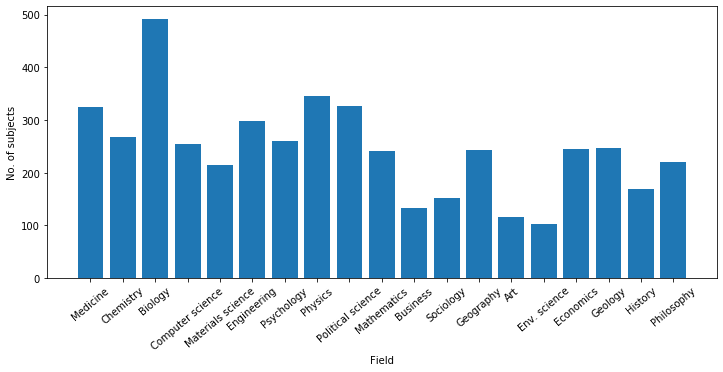
\includegraphics[width=\textwidth]{figures/unsupervised_approach/subjects_per_field.png}
    \caption{Number of subject that descend of each of the fields.}
    \label{fig:subjects_per_field}
\end{figure}

2,157 subjects were extracted with this procedure, which results on an average of 114 subjects per field. We could extract 200 subjects for all fields except for \textit{Environmental Science}, \textit{Business}, \textit{Sociology}, \textit{Art} and \textit{History}. On the other hand, \textit{Medicine}, \textit{Biology} and \textit{Physics} have more than 300 descendant subjects under the ones we have collected. This is because subjects can descend from multiple fields. For example, \textit{Neuroscience} can be classified under \textit{Biology}, \textit{Medicine} and \textit{Computer science}. The number of subjects per field can be seen in figure \ref{fig:subjects_per_field}.

All 25 subjects of the second level have been picked, followed by 1,999 of the third level, 108 of the fourth, and 6 of the fifth. On average, subjects are assigned to 197,180 publications. No subjects are assigned to less than 100 documents, as this was a requirement in the extraction procedure. Regarding the hierarchy of the subjects, all but 13 of them have ancestors in all levels above them. Two subjects of the third, \textit{Sensitivity} and \textit{Boundary}, are directly linked to fields. \textit{Sensitivity} is a descendant of both \textit{Engineering} and \textit{Mathematics}, whereas \textit{Boundary} descends from \textit{Mathematics}. The remaining eleven subjects that don't have ancestors in all previous levels belong to the fourth level. All of them descend from subjects of the second level, thus skipping the third level.
\subsection{Research question} \label{problem_rq}

The research question this thesis attempts to answer is the following:

\begin{quote}
    \textit{What family of approaches, supervised or unsupervised, is more suitable for performing subject indexing in small and multidisciplinary repositories?}
\end{quote}

The distinction between supervised and unsupervised is made in the field of machine learning, which is the paradigm we plan on implementing, as it is the most powerful method according to the literature (see chapter \ref{subject_indexing}).

Supervised approaches are those that learn through examples. They receive input-output pairs, and they are optimized to output what is expected for each of those inputs. The input-output pairs are usually called \textit{training data}, and the final performance of the model largely depends on its quality. Unsupervised approaches are fundamentally opposite: they learn to perform an action directly from the data, without any examples. They are based on the intuition that the data itself contains the necessary information for the model to perform its task
\cite{hinton1999unsupervised}.

Both approaches are interesting for our use case because of the size and content of our dataset. Supervised approaches have been proven more effective in most scenarios, and also in \acrshort{si} tasks. However, they require accurate training data, which is not available in our use case. The assignments of \acrshort{mag} are reported to be 80 \% accurate. Therefore, an unsupervised approach may offer better results in our use case. In this thesis, we explore the advantages and disadvantages of both approaches. We focus especially on \acrshort{si} accuracy, which is the ultimate goal, but also discuss other aspects such as the complexity of the implementation and computational cost.

\section{Repository analysis} \label{repo_analysis}

This thesis comprises the documents on the repositories of the \acrshort{tu}, \acrshort{hu} and \acrshort{fu}. The repositories are called depositonce, edoc and refubium, respectively. There are 62,507 documents\footnote{As of 26/05/2021.} among the three repositories. As mentioned in section \ref{problem_scope_docs}, we are only interested in theses and publications written in English. We thus discard documents referring to research data, university related documents and others, leaving us with 29,399 documents, with 47 \% of them belonging to refubium and 63 \% being publications. The analysis presented in this chapter only considers these relevant documents.

We start by exploring the existing subjects in section \ref{repo_analysis_subjects}, which are at the core of this thesis. 81 \% of them appear in only one document, and only 5 \% in more than three, which renders them useless for navigating the repositories. We also present the distribution of the \acrfull{ddc} subjects. \textit{Science}, \textit{Social Sciences} and \textit{Technology} cover 83 \% of all the relevant documents.

We then look at venues (section \ref{repo_analysis_venues}) and contributors (section \ref{repo_analysis_contributors}), which are also useful to relate documents to one another. Venues are assigned to four documents on average, and only 2 \% of the publications don't have one. Referees and advisors, which we will use as a replacement for venues when considering theses, also offer a good coverage of the theses, with all but 4 \% of the theses having an advisor or a referee.

Finally, in section \ref{repo_analysis_data}, we analyze the actual data that will be used to perform \acrshort{si}: the titles and abstracts of the documents. All documents in the repositories are required to have a title, so all the documents have one. Abstracts, on the other hand, are optional. 6 \% of the relevant documents don't have one. In this final section, we also discuss how certain titles and abstracts are tagged as being written in English when they are not. When running a language detection algorithm, we find out that 320 abstracts are not actually written in English. We try to solve this issue for detecting the language of the other abstracts of the documents, which are tagged as being written in other languages.

\subsubsection{Set of subjects} \label{problem_scope_subjects}

Our dataset comprises considerably fewer documents than \acrshort{mag} (tens of thousands instead of hundreds of millions). Given that our goal is to relate documents to one another through their content, and we are focusing on small repositories, we don't require such granular subjects. If we used all the \acrshort{mag} subjects, most of them would be left unassigned, and many others would be assigned only once. We therefore pick a subset of these subjects.

\acrshort{mag} structures their set of subject as a hierarchy, where the first level comprises 19 subjects, which we call fields for clarity. Under each field, there exist five further hierarchy levels. We extract the subjects from OpenAlex, which is currently the best data source for subjects and publications of \acrshort{mag} (see section \ref{mag_access_data}).

In section \ref{problem_scope_subjects_retrieve}, we present our subject retrieval procedure. We discuss how many subjects we retrieve per field, and on what conditions we pick among the thousands of candidates. Then, we present the resulting set of subjects in section \ref{problem_scope_subjects_result}.

\paragraph{Subject retrieval} \mbox{} \label{problem_scope_subjects_retrieve}

We have extracted up to 200 descendants of each of the 19 fields. We consider how many publications a subject has been assigned to, assuming that popular subjects are more likely to appear in the repositories. We have tried different thresholds for how many assignments a subject needs to be considered, to strike a balance between picking subjects from the upper levels, which are more general, and picking subjects that are popular.

The problem is that the fields differ in popularity. For example, \textit{Medicine} has more than 200 subjects in the third level with more than 25k works, whereas \textit{Environmental science} only has 31 across all levels. We therefore start with a larger limit, iterate over all levels and all fields, and decrease the limit before iterating again. We first iterate through the descendants of each field and add subjects that are assigned to at least 25,000 publications. If the list of a field does not include 200 subjects after this iteration, we do so again, considering subjects assigned to at least 10,000. We repeat this procedure with 5,000, 1,000 and 100 assignments. When we iterate through the subjects of a field, we start by the second level and descend if necessary.

To avoid uninformative Wikipedia texts such as ``Emotionalism may refer to:'', we discard subjects whose description says ``Wikimedia disambiguation page'' or ``Wikimedia glossary list article''. The description from a subject comes from the corresponding Wikidata link, through which we later extract the Wikipedia link. For each subject that meets these requirements, we append it to all the fields it has in its list of ancestors, to keep the number of subjects as low as possible while providing good coverage of the fields.

\paragraph{Resulting set of subjects} \mbox{} \label{problem_scope_subjects_result}

\begin{figure}
    \centering
    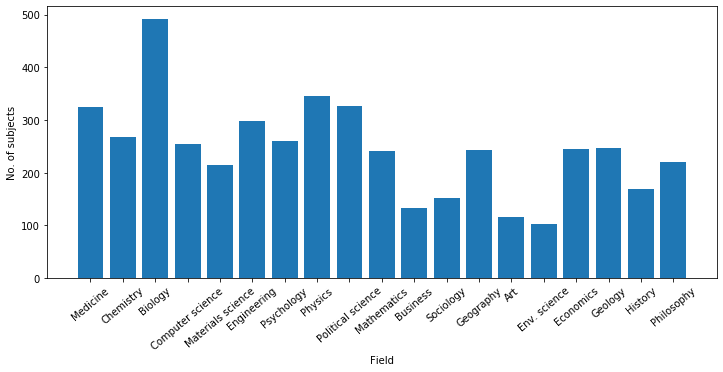
\includegraphics[width=\textwidth]{figures/unsupervised_approach/subjects_per_field.png}
    \caption{Number of subject that descend of each of the fields.}
    \label{fig:subjects_per_field}
\end{figure}

2,157 subjects were extracted with this procedure, which results on an average of 114 subjects per field. We could extract 200 subjects for all fields except for \textit{Environmental Science}, \textit{Business}, \textit{Sociology}, \textit{Art} and \textit{History}. On the other hand, \textit{Medicine}, \textit{Biology} and \textit{Physics} have more than 300 descendant subjects under the ones we have collected. This is because subjects can descend from multiple fields. For example, \textit{Neuroscience} can be classified under \textit{Biology}, \textit{Medicine} and \textit{Computer science}. The number of subjects per field can be seen in figure \ref{fig:subjects_per_field}.

All 25 subjects of the second level have been picked, followed by 1,999 of the third level, 108 of the fourth, and 6 of the fifth. On average, subjects are assigned to 197,180 publications. No subjects are assigned to less than 100 documents, as this was a requirement in the extraction procedure. Regarding the hierarchy of the subjects, all but 13 of them have ancestors in all levels above them. Two subjects of the third, \textit{Sensitivity} and \textit{Boundary}, are directly linked to fields. \textit{Sensitivity} is a descendant of both \textit{Engineering} and \textit{Mathematics}, whereas \textit{Boundary} descends from \textit{Mathematics}. The remaining eleven subjects that don't have ancestors in all previous levels belong to the fourth level. All of them descend from subjects of the second level, thus skipping the third level.
\subsection{Publishing venues} \label{repo_analysis_venues}

The venue where a publication was published is important information that relates documents to one another regarding the topics they discuss. For example, the publishing venue of an article is a journal. Theses don't have publishing venues, as they serve another purpose (namely, evaluating the student's knowledge and ability). In this section, we discuss the publishing venue for each type of document. Given that how the venue is stored differs depending on the repository, we look at each of them separately.

Table \ref{tab:publishing_venues} shows the most common field names per publication type and repository. For example, all 3,233 articles present in depositonce have the name of the journal they were published in stored in a field called \textit{``journalTitle''}. Books in refubium often have two fields named \textit{``series''}, one for the name of the series and the other for the issue number that corresponds to the book.

The most popular venue is called ``Sonderforschungsbereich 649: Ökonomisches Risiko'' which appears on 809 publications of edoc. The second most popular venue is also a ``Sonderforschungsbereich'' of the \acrshort{hu} (which means ``research area in English'') and it appears in 583 publications. The third one is the first real publishing venue: ``PLoS ONE'', with 533 publications.

On average, venues appear on 4.2 publications. There are 4,418 venues present across all three repositories, 2,867 of which (65 \%) are only assigned to one publication. From this follows that 2,867 publications (15 \%) have a venue which they don't share with any other publication. As shown in figure \ref{fig:pubs_venue_alone}, more than half of these publications belong to refubium. Furthermore, 292 publications (2 \%) don't have a venue, almost half of them belonging to depositonce. The amount of these publications that belong to each repository is illustrated in figure \ref{fig:pubs_with_no_venue}.

\begin{table}
\centering
\begin{tabular}{|c|c|c|c|c|}
\hline
\thead{Doc. type} & \thead{Repository} & \thead{\# docs} & \thead{Field name} & \thead{\# fields} \\
\hline\hline
\multirow{3}{*}{Article} & depositonce & 3233 & journalTitle & 3233 \\ \cline{2-5}
& edoc & 1904 & container-title & 1846 \\ \cline{2-5}
& refubium & 7519 & journalTitle & 3517 \\ \cline{2-5}
\hline
\multirow{3}{*}{Book part} & depositonce & 155 & bookTitle & 155 \\ \cline{2-5}
& edoc & 160 & container-title & 214 \\ \cline{2-5}
& refubium & 172 & bookTitle & 109 \\ \cline{2-5}
\hline
\multirow{3}{*}{Book} & depositonce & 91 & series & 118 \\ \cline{2-5}
& edoc & 2128 & container-title & 2076 \\ \cline{2-5}
& refubium & 1184 & series & 2211 \\ \cline{2-5}
\hline
\multirow{3}{*}{Conference Obj.} & depositonce & 465 & series & 450 \\ \cline{2-5}
& edoc & 489 & container-title & 993 \\ \cline{2-5}
& refubium & 378 & series & 0 \\ \cline{2-5}
\hline
\end{tabular}
\caption{Field names where the publishing venues are stored per document type and repository.}
\label{tab:publishing_venues}
\end{table}

\begin{figure}
  \begin{subfigure}[t]{0.45\textwidth}
    \centering
    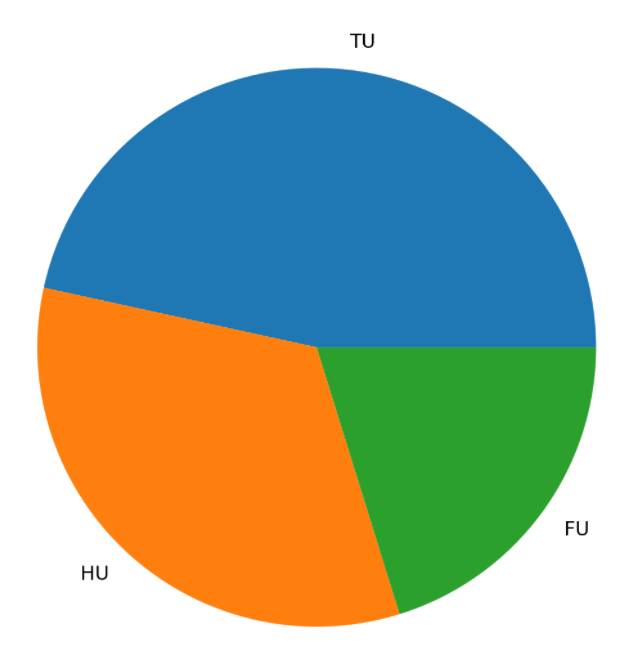
\includegraphics[width=\textwidth]{figures/repository_analysis/pubs_with_no_venue.PNG}
    \caption{Publications with no venue}
    \label{fig:pubs_with_no_venue}
  \end{subfigure}
  \hfill
  \begin{subfigure}[t]{0.41\textwidth}
    \centering
    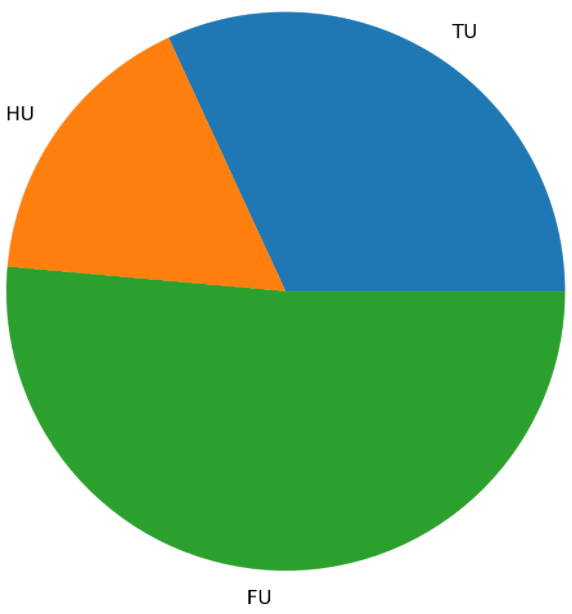
\includegraphics[width=\textwidth]{figures/repository_analysis/pubs_venue_alone.PNG}
    \caption{Publications that don't share the venue with any other publication.}
    \label{fig:pubs_venue_alone}
  \end{subfigure}
  \caption{Pie charts about the venues of the publications.}
\end{figure}
\subsection{Contributors} \label{repo_analysis_contributors}

\begin{figure}
    \centering
    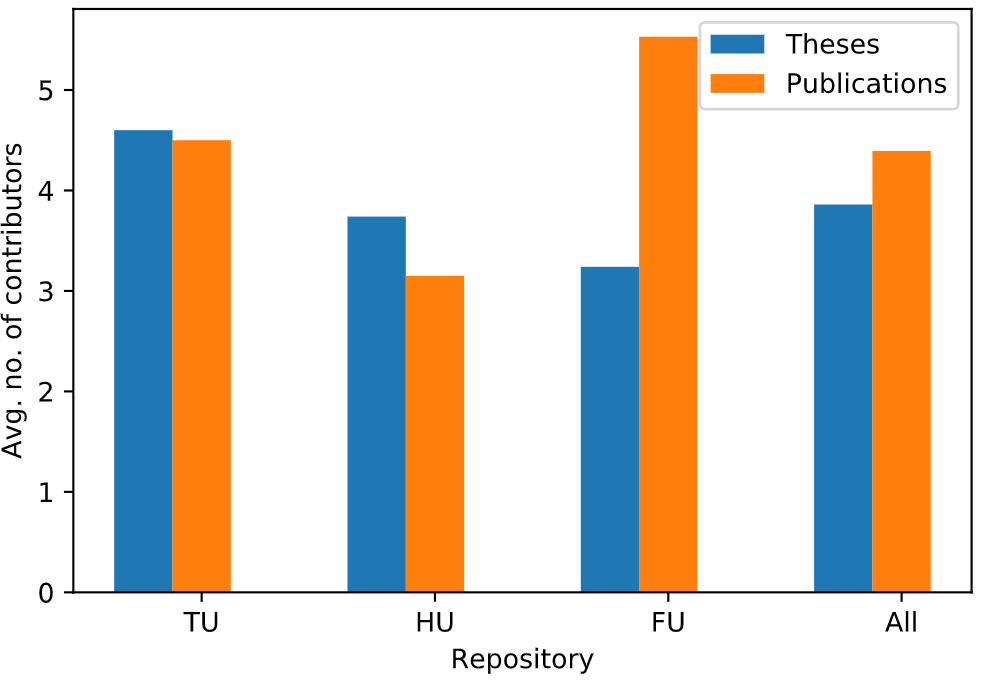
\includegraphics[width=.7\textwidth]{figures/repository_analysis/avg_contributors.PNG}
    \caption{Avg. number of contributors per document type and repository.}
    \label{fig:avg_contributors}
\end{figure}

In this section, we look at what types of contributors are present in the repositories and how often they occur. On average, documents of depositonce, edoc and refubium have 4.5, 3.4 and 4.7 contributors, respectively. In depositonce, publications and theses offer similar average numbers of contributors. In edoc, there are 0.5 more contributors in theses than in publications. In refubium it is the other way around: publications have 2.3 more contributors than theses on average. These numbers are shown illustrated in figure \ref{fig:avg_contributors}.

Regarding the types of contributors, publications usually include only the author. Edoc includes a significant number of editors, as shown in figure \ref{fig:author_types}. Theses, on the other hand, have other important types of authors: referees and advisors. After analyzing the authors, we will look at these two author types in the following sections. They are relevant because they could be used to relate documents, the same role that venues play for publications.

\begin{figure}
    \centering
    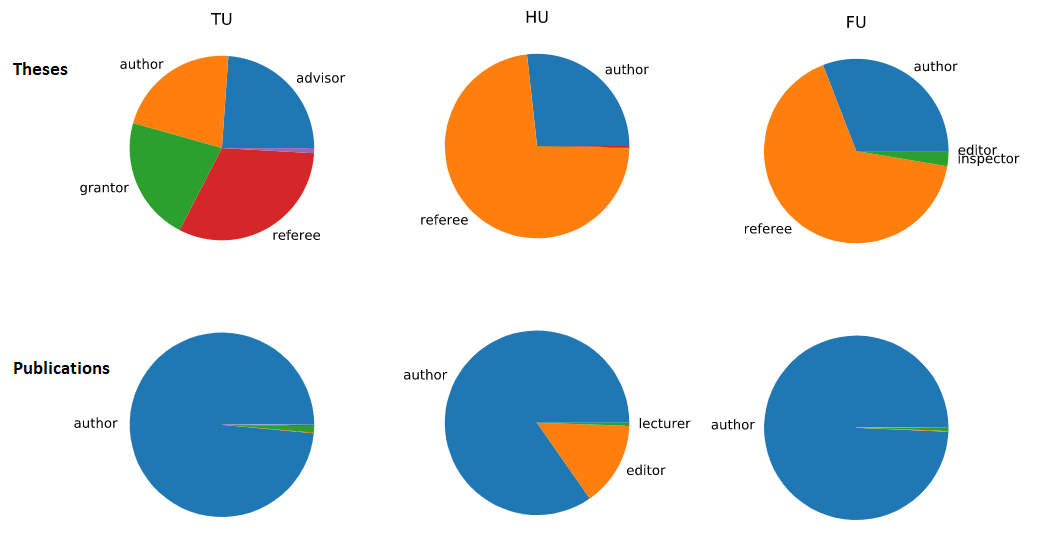
\includegraphics[width=\textwidth]{figures/repository_analysis/author_types_pretty.png}
    \caption{Author types that appear on each repository depending on the document type.}
    \label{fig:author_types}
\end{figure}


\subsubsection{Authors}

Authors are the most important contributors, as they are responsible for the content of the document. Only 207 out of the 29,399 documents don't have an author (0.7 \%), all of them being publications and 144 of them belonging to refubium. Publications have on average more authors than theses. Out of all 10,773 theses, only two of them have more than 1 author. Both of them belong to edoc. In contrast, 80 \% of the publications have multiple authors. This difference is expected, as students are usually required to write a thesis by themselves, whereas researchers often collaborate and publish their work together.

Authors of theses rarely have more than one thesis, as shown in figure \ref{fig:n_publications_per_author}. In total, 56 alumni have authored multiple theses. The real number is lower, as a quick check of some of them reveals the existence of duplicates. The ones that do have two theses to their name are Master's students that went on to pursue a PhD. On the other hand, the researchers present in the repositories have authored on average 1.6 publications. The two researchers with the most publications are Kai Nagel, from the \acrshort{tu} Berlin, and Wolfgang Härdle, from the \acrshort{hu} Berlin. Both have authored 143 publications. Still, more than 77 \% of the researchers have authored only one publication. Figure \ref{fig:n_publications_per_author} shows the distribution of researchers among the number of publications they have authored.

\begin{figure}
    \centering
    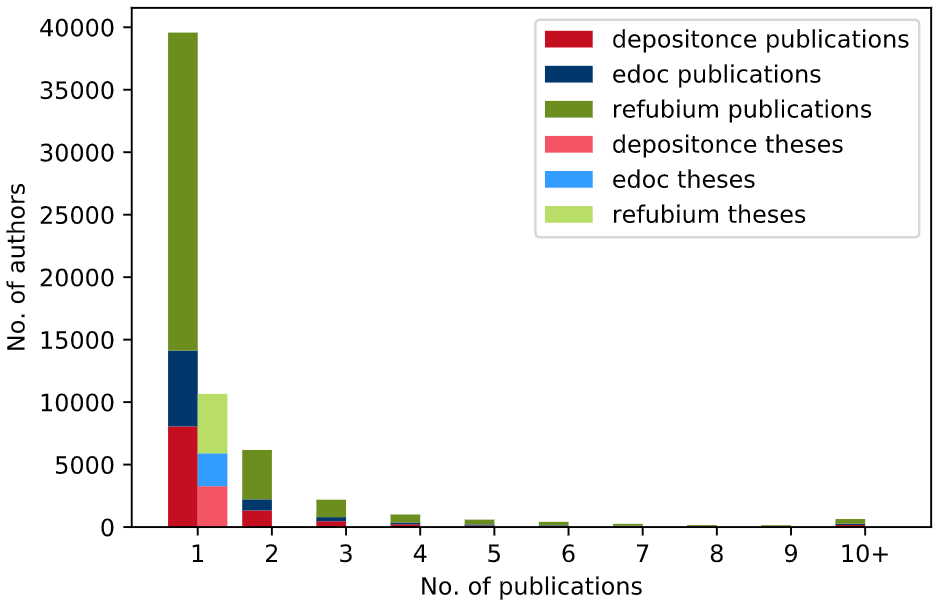
\includegraphics[width=.7\textwidth]{figures/repository_analysis/n_publications_per_author.PNG}
    \caption{No. of authors per no. of publications.}
    \label{fig:n_publications_per_author}
\end{figure}


\subsubsection{Referees}

Referees are in charge of evaluating the student's work and assigning a grade to the submitted thesis. Thus, every thesis requires at least one referee. Both edoc and refubium provide referees for almost all their theses. Only 39 and 41 documents are missing a referee, respectively. On the other hand, 1,442 theses of depositonce do not include a referee, which amounts to 19 \% of all theses.  These and all other facts presented in this section are summarized in table \ref{tab:referees}.

A caveat to the referees of refubium is the presence of ``N.N.'' as the most popular referee, appearing 1,126 times. It stands for the Latin phrase \textit{Nomen Nescio}, which means ``unknown person''. Therefore, all theses of refubium that include ``N.N.'' or variations of it can also be seen as theses without a referee. Then, refubium has 662 theses without a referee instead of 41, which amounts to 5 \% of all its theses. In total, depositonce comprises 4,780 referees, 2,388 of which are distinct. In edoc there are 7,289 referees, of which 3,390 are distinct. In refubium there are 9,133 referees and 4,863 distinct ones.

The documents that do have a referee often include more than two. On average, theses in depositonce include 2.6 referees, those of edoc 2.8 and those of refubium 2.2. Please note that theses averages don't take into account theses that have zero referees. The \textit{Nomen Nescio} referees of refubium are also ignored. The referees are professors of the universities and therefore appear frequently on the repositories, as they evaluate numerous theses. On average, professors appear two times in the repositories as referees. In depositonce there are 57 referees who have evaluated more than ten theses; in edoc there are 97 such referees and in refubium, 88. The most recurrent referees of each repository are Rupert Mutzel (FU Berlin), who has been a referee for 72 theses Wolfgang Härdle (HU Berlin), who appears on 60 theses and Peter Neubauer (TU Berlin), who appears on 45 theses.

\begin{table}[]
    \centering
    \begin{tabular}{|c|c|c|c|c|}
    \hline
         \thead{Repository} & \thead{\# referees} & \thead{\# distinct  \\ referees} & \thead{Avg. \# \\ referees \\ per thesis} & \thead{\# theses \\ without \\ a referee} \\
         \hline
         depositonce & 4,780 & 2,338 & 2.6 & 1442 (19 \%) \\
         \hline
         edoc & 7,289 & 3,390 & 2.8 & 39 (1 \%) \\
         \hline
         refubium & 9,133 & 4,863 & 2.2 & 662 (5 \%) \\
         \hline
    \end{tabular}
    \caption{Facts regarding the referees of theses.}
    \label{tab:referees}
\end{table}

\subsubsection{Advisors}

Advisors are also a building block of a thesis. They are experts on the topics handled by the thesis they advise on, and also help the student with the writing process. All facts presented in this section are summarized in table \ref{tab:advisors}. Only depositonce has a maintained list of advisors. All but 124 theses (4 \% of all theses) have at least one advisor. edoc only has 13 advisors and refubium has none. Coincidentally, depositonce is the repository where the referees are not as well maintained as in the other repositories. It seems that users of depositonce care more about advisors, and users of edoc and refubium about referees.

Students usually have just one advisor. In depositonce, theses include on average 1.1 advisors; in edoc, 1.3 advisors. Regarding how many theses share the same advisor, the average for depositonce is 3.3 theses per advisor. For edoc, the average is 1.5. Depositonce has 84 advisors that appear on more than ten different theses. edoc, on the other hand, has none. The advisor of depositonce with the most theses is Klaus-Robert Müller, who has advised 47 theses. For edoc, the most recurrent advisor is Wolfgang Härdle, who has advised 6 theses.

\begin{table}
    \centering
    \begin{tabular}{|c|c|c|c|c|}
    \hline
         \thead{Repository} & \thead{\# advisors} & \thead{\# distinct  \\ advisors} & \thead{Avg. \# \\ advisors \\ per thesis} & \thead{\# theses \\ without \\ an advisor} \\
         \hline
         depositonce & 3,603 & 1,080 & 1.1 & 124 (4 \%) \\
         \hline
         edoc & 19 & 13 & 1.3 & 2,659 (99 \%) \\
         \hline
         refubium & 0 & 0 & 0 & 4,815 (100 \%) \\
         \hline
    \end{tabular}
    \caption{Facts regarding the advisors of theses.}
    \label{tab:advisors}
\end{table}

\subsection{Titles and abstracts} \label{repo_analysis_data}

As mentioned in the introduction, we consider the titles and abstracts of the documents to represent them. In this section, we will present some facts about these two fields, regarding how often they are left empty in the repositories and other noise factors in our corpus, such as the hundreds of texts that are tagged as being written in English when they are not.

\subsubsection{Fill quota}

The title is a required field in all three repositories and is therefore present for all the documents of our corpus. Abstracts, on the other hand, are optional fields. It is empty in 135 of the 7,438 documents of depositonce (1.8 \%), in 922 of the 7,497 documents of edoc (12.3 \%) and in 776 of the 14,464 documents of refubium (5.4 \%). In total, 1,833 of 29,399 documents (6.2 \%) don't have an abstract. Most of the documents that are missing the abstract are publications. None of the 135 documents of depositonce that don't have an abstract are theses. In edoc, only 25 of the 922 documents (2.7 \%) without an abstract are theses; in refubium, 11 of 765 (1.4 \%).

\subsubsection{Foreign languages}

Looking at the data reveals that there are several titles and abstracts which should be written in English (as stated in the tags of the field) but are actually in German. This is the case for 678 titles (2.3 \% of all titles) and 320 abstracts (1.1 \%). Out of the 678 titles, 542 are written in German (80 \%). 381 of these belong to refubium, 90 to depositonce and 71 to edoc. Some titles included in this list are actually in English, but have been misclassified due to their brevity. For example, the two titles that are considered to be written in Polish are ``Przy Bazantarni, Warsaw'' and ``Democrazy ?!''. The second one is clearly not Polish, but given that the word ``Democrazy'' ends like ``Przy'', a misclassification can happen.

Detecting the language of the abstracts is more reliable given the larger size of the text. Out of the 320 abstracts that are not written in English, 319 of them are in German and 1 in Polish. Again, many of the abstracts that are considered to be written neither in German nor English are often in English, but misclassified due to their brevity.

The difference in length between texts written in German and those written in other languages (excluding English) is illustrated in figure \ref{fig:foreign_languages}. German titles comprise 85 characters on average, whereas those in other languages comprise 18 characters. The difference is even more clear when looking at abstracts: German abstracts are 2,682 characters long on average, and those in other languages only 965 characters long. This difference in length supports our hypothesis that texts that are classified as other languages other than German are often errors that occur because of the brevity of the text.

\begin{figure}
    \centering
    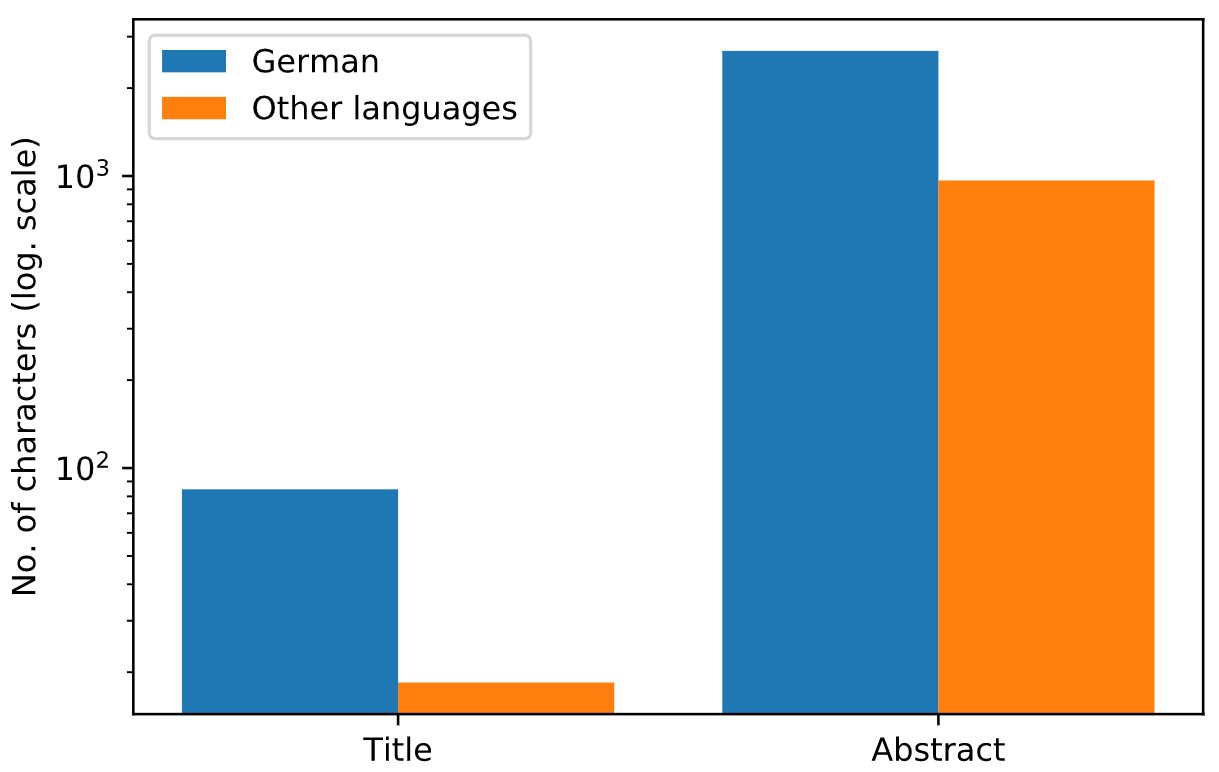
\includegraphics[width=.7\textwidth]{figures/repository_analysis/foreign_languages.PNG}
    \caption{Lengths of titles and abstracts that are not written in English.}
    \label{fig:foreign_languages}
\end{figure}

We determined the language of the texts using the Python package \textit{langdetect}\footnote{\url{https://github.com/Mimino666/langdetect}}, which uses a naive Bayes filter to identify the most probable language out of 53 options. We run the function \textit{detect\_langs} 10 times for each text: a text is written in a foreign language if the probability of the first result is always above 99 \% and the language remains the same throughout all 10 executions. We then use langdetect again to retrieve English texts from the repositories that have been tagged incorrectly (e.g. English texts where the language is said to be German). After extracting all titles and abstracts of each document, we run the language detection procedure described above for each of the possibilities and return the one in English, if any.

Doing so returns English titles for 443 out of the 678 documents (65 \%) with titles in foreign languages and English abstracts for 306 out of the 320 documents (96 \%). When looking at the tags of these retrieved fields, we see that most of them incorrectly state that the text is in German. This is the case for 274 out of the 306 found abstracts. We then run the language detection procedure one again on the improved data. Although we expect to encounter more texts in English, we cannot assume that the number of English texts is now the number of English texts in the original data minus the number of the English texts retrieved with the language detection procedure because of the randomness of the detection model.

This final run shows that 271 titles  (0.9 \%) and 14 abstracts (0.04 \%) are written in foreign languages. 177 of the 271 titles (65 \%) in foreign languages are in German, and all abstracts but one (which is written in Polish) are in German. With this language detection procedure, we have been able to improve the quality of our data, reducing the number of texts written in foreign languages. We have retrieved English texts for 409 titles and 306 abstracts that were previously in foreign languages because of incorrect language tags in the data. 

Please note that these numbers are not fully reliable, given that the model is not always able to correctly predict the language of a text. This can be seen in the number of titles that were deemed to be in foreign languages when looking for alternative titles and those detected in the final run. The first round showed that 235 titles were in foreign languages. Running the same detection procedure again output 271 titles. On the other hand, the detected language for the abstracts remained the same in both runs. This shows that the length of the text is an important factor when evaluating the performance of the language detection model.

\section{Related work on unsupervised approaches} \label{subject_indexing}

\acrfull{si} has been a topic in academia well before it became important in the digital realm, as it was relevant for the organization of conventional libraries. The current ISO standard (ISO 5963:1985) defines \acrshort{si} as a three-step process:

\begin{enumerate}
    \item Determine the content of a document.
    \item Perform conceptual analysis to extract concepts from the content.
    \item Translate the concepts into a controlled vocabulary.
\end{enumerate}

Automatic Subject Indexing (ASI) occurs when machines perform this \acrshort{si} procedure instead of humans. There are also approaches in which machines aid humans in the process of indexing, called Machine-Aided Indexing (MAI) or Computer-Aided Indexing (CAI). We will however refer to the automatic task as \acrshort{si}, which is how it is usually referred to in the literature. Indexing can be differentiated from classification in its purpose \cite{golub2019automatic}. It focuses on facilitating the retrieval of a document, assuming that users will look for it from different perspectives. Classification, on the other hand, tries to clearly categorize the documents, using fewer subjects per document and aiming for the highest precision instead of covering a broader spectrum of possible queries.

In this chapter, we review the literature on this topic. We first summarize the different ways in which \acrshort{si} methods can be classified, which revolve around two conditions: the existence of training data, which enables the implementation of supervised \acrlong{ml} algorithms, and the availability of a set of subjects. If such a set does not exist, the subjects must be extracted from the texts.

Afterwards, we present the common challenges that \acrshort{si} methods face. Heterogeneous documents increase the complexity of performing \acrshort{si}, whereas the number of documents hinders the performance of many methods. Also, texts written in different styles pose different problems. Subjects can also pose challenges, such as their uneven assignment distribution and how their distribution changes over time. Training data may also suffer from this distribution drift over time, as well as label noise due to inconsistencies between different human indexers.

In the next section, we present several unsupervised approaches to \acrshort{si} that use an existing set of subjects. We first present two approaches that are popular in the literature: string matching methods that map subjects to documents, relying on the quality of the set of subjects to achieve a high matching rate, and the application of \acrlong{lda} for subject indexing scenarios where subjects already exist.

We then present the \acrfull{mag} in section \ref{subject_indexing_mag}. The \acrshort{mag} is, to the best of our knowledge, the most successful application of unsupervised subject indexing for scientific texts. Its use case closely resembles ours, as their dataset comprises documents from various scientific fields. They are also the source for our set of subjects. Their indexing procedure consists of vectorizing documents and subjects and computing the cosine distances between them to discover the similarity between each document and each subject. In this thesis, we implement the \acrshort{mag} indexing procedure, as its scenario closely resembles ours, and it is proven to be accurate. The other approaches discussed in this chapter neither as accurate, nor as well tested for scientific texts. The \acrshort{mag} is widely used in academia to this day, so we safely assume its indexing method was successful.

\subsection{Classifications of methods} \label{subject_indexing_types}

% Subject indexing methods can be classified in various manners. For instance, approaches can be classified regarding the origin of the used subjects \cite{golub2019automatic}. Derived \acrshort{si} extracts the subjects from the document itself, while assigned \acrshort{si} maps a fixed set of subjects to the given document.

In this section, we give an overview of the different classifications of \acrshort{si} methods that we have found in the literature. They all revolve around the existence of a \acrfull{kos}, and the availability of training data.

\subsubsection{Golub's classification} \label{subject_indexing_golub}

Golub classifies \acrshort{si} approaches regarding the application purpose, the amount of research backing it and the paradigm used (\acrlong{ml} or string matching, essentially) \cite{golub2019automatic}. It classifies \acrshort{si} approaches into three groups.

\textit{Document clustering} is suited for cases where there is neither training data nor a \acrshort{kos}. Clustering algorithms group documents according to a given similarity metric. They can be used to group documents that belong to the same topic. For example, the similarity metric may measure the amount of mutual information between documents \cite{slonim2002unsupervised}. Document clustering poses two challenges: the resulting structures may be hard to understand \cite{chen2000bringing}, and they can also change once more documents are added. The second challenge is that the assignment of topics to clusters may be unclear and require human intervention.

\textit{Text categorization} is used when both training data and a \acrfull{kos} are available. It consists of a supervised \acrshort{ml} algorithm that learns the features of the subjects of the \acrshort{kos} from the already assigned documents. Once the algorithm is trained, these features will enable it to map subjects to new documents. It can be applied for \acrshort{kos}s that order subjects in hierarchies. Furthermore, doing so may improve the classification accuracy of the method \cite{chen2000bringing}. The third group, \textit{document classification}, is similar to text categorization, but differs from it in the quality of the \acrshort{kos}. The higher \acrshort{kos} quality enables document classification methods to rely on string matching to map subjects to documents, instead of complex machine learning algorithms \cite{khoo2015augmenting}.

\subsubsection{Medelyan's classification} \label{subject_indexing_medelyan}

Medelyan is the author of KEA++ \cite{medelyan2008domain}, a keyphrase extraction algorithm, and also of Maui \cite{medelyan2009human}, another popular indexing algorithm. She differentiates between two types of subject indexing approaches, which she then combines to develop the paradigm used by KEA++.

\textit{Keyphrase extraction} consists of searching for relevant words or phrases in documents. They use solely intrinsic information, such as word frequency or document length. This type of indexing is free in the sense that any keyphrases can be extracted. There is no set of possible keyphrases, i.e. a \acrshort{kos}. The disadvantage of this kind of indexing methods is that the keyphrases won't necessarily have the same form (only words in singular, for example). Also, the presence of undetected synonyms may reduce the quality of the resulting index.

\textit{Term assignment}, on the other hand, uses a \acrshort{kos}. These approaches often rely on string matching to find the keyphrases of the \acrshort{kos} in the documents. The most recent efforts in this field use machine learning methods to map keyphrases to documents. The disadvantage of using classifiers is that they require a lot of training data, whereas string matching method don't require any.

\textit{Keyphrase indexing} combines the two approaches described above, which may be seen as complementary in terms of their strengths and weaknesses. The basic procedure is as follows: given a document, its candidate phrases are first mapped to the keyphrases of the \acrshort{kos} to remove uninformative words and avoid polysemy and synonyms; then, the remaining candidates are analyzed to extract the relevant ones.

In KEA++ \cite{medelyan2008domain}, the analysis of the candidates consists of computing four features for each candidate. These features are fed to a \acrshort{ml} algorithm, which outputs a boolean value stating if the corresponding candidate should be assigned to the document or not. The \acrshort{ml} algorithm is supervised, i.e. it requires a training set. KEA++ uses the Naive Bayes algorithm, which offered the best results when compared with other supervised \acrshort{ml} algorithms like the SVMs and decision trees.

\subsubsection{Töpfer's classification} \label{subject_indexing_toepfer}

Töpfer differentiates between lexical and associative indexing approaches and concludes that both approaches complement each other, which is an argument in favor of fusion architectures, the third member of his classification of \acrshort{si} methods \cite{toepfer2020fusion}. We will look at these three groups in this section.

\textit{Associative approaches} find correlations between words \cite{suominen2019annif} by computing co-occurrence statistics, which allow the methods to identify references to the subjects of the \acrshort{kos}. These methods require training data to learn the mappings. Subjects that do not appear in the training data cannot be assigned to any documents, because the model has not learned weights for them. This means that associative approaches require a lot of training data that is well distributed among the subjects, as it is not able to predict unseen subjects.

\textit{Lexical approaches} map salient terms in the document to the subjects using a trained model \cite{suominen2019annif}. KEA++ \cite{medelyan2008domain}, presented in the previous section, is a lexical approach. Because the weights and the threshold are shared by all subjects, lexical models can be used to assign previously unseen subjects. The parameter estimations are reliable because the values computed for each candidate are usually non-vanishing \cite{toepfer2020fusion}. Therefore, not so much training data is required.

Both approaches may lead to low recall. Associative approaches may have low recall when the training data is insufficient. This is likely to be the case because of \textit{Zipf's law}: when ranked by frequency, the frequency of each subject is half of its predecessor. On the other hand, lexical systems may suffer from low recall when the \acrshort{kos} lacks synonyms, which could hamper the hit rate of the string matching step.

\begin{figure}
    \centering
    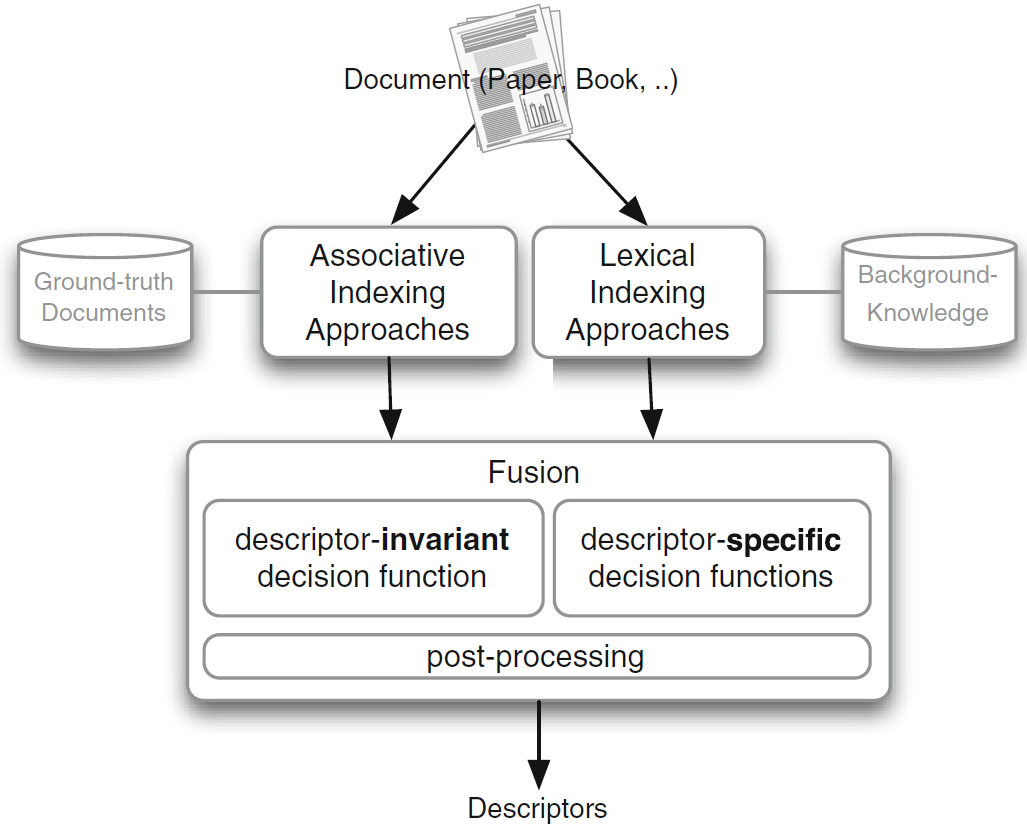
\includegraphics[width=.5\textwidth]{figures/related_work/fusion_architecture.PNG}
    \caption{Schema of a fusion architecture. From \cite{toepfer2020fusion}.}
    \label{fig:fusion_architecture}
\end{figure}

\textit{Fusion architectures} combine lexical and associative indexing systems. Their goal is to gather the advantages of both methods, which were shown to be complementary in the previous section, in one system. Figure \ref{fig:fusion_architecture} shows a schema of the architecture. The decision function, which can be either invariant or specific regarding the subjects, merges the results of the indexing systems into a single set of subjects, which is then assigned to the document after some optional post-processing. The descriptor-invariant decision function may be used for all descriptors, also unseen ones. The descriptor-specific decision function uses the background knowledge and the ground-truth documents to decide on the output.



\subsubsection{Comparison of classifications}

The usage of a \acrshort{kos} and the requirement of training data are the two distinguishing factors of the classifications. These are summarized in table \ref{tab:subject_indexing_classifications}. We will now look at them as a whole and establish relationships between them when possible.

\begin{table}
\centering
\begin{tabular}{|c|c|c|c|c|}
\hline
\thead{Author} & \thead{Group} & \thead{KOS} & \thead{Tr. data} & \thead{Method} \\
\hline\hline
\multirow{3}{*}{Golub} & Text categorization & Yes & Yes & ML algorithm \\ \cline{2-5}
& Document clustering & No & No & ML algorithm \\ \cline{2-5}
& Document classification & Yes & No & String matching \\ \cline{2-5}
\hline
\multirow{3}{*}{Medelyan} & Keyphrase extraction & No & No & String matching \\ \cline{2-5}
& Term assignment & Yes & Yes & Any \\ \cline{2-5}
& Keyphrase indexing & Yes & Yes & ML algorithm \\ \cline{2-5}
\hline
\multirow{3}{*}{Töpfer} & Associative methods & Yes & Yes & ML algorithm \\ \cline{2-5}
& Lexical methods & Yes & Yes & Both \\ \cline{2-5}
& Fusion architecture & Yes & Yes & Both \\ \cline{2-5}
\hline
\end{tabular}
\caption{Summary of the SI classifications.}
\label{tab:subject_indexing_classifications}
\end{table}

Golub's \textit{document clustering} and Medelyan's \textit{keyphrase extraction} are the only categories that require neither a \acrshort{kos} nor assigned documents as training data. They differ mainly in their objective: document clustering focuses on the subjects that relate documents, whereas keyphrase extraction looks at each document individually, looking for its most significant subjects.

Töpfer mentions Medelyan's models (KEA++ \cite{medelyan2008domain} and Maui \cite{medelyan2009human}) as examples of \textit{lexical methods}. Given that, according to Medelyan's classification, they belong to the \textit{keyphrase indexing} category, we can establish a relationship among these two categories. Furthermore, \textit{keyphrase indexing} arises from combining the other two categories of Medelyan's classification (\textit{term assignment} and \textit{keyphrase extraction}). Therefore, all three categories from Medelyan can be placed under Töpfer's lexical methods. Golub's \textit{text categorization} also requires training data and a \acrshort{kos}, and uses an \acrshort{ml} algorithm as well.

Finally, Medelyan mentions that \textit{term assignment} methods only require training data if an \acrshort{ml} algorithm is going to be used. If string matching is used, no training data is required. In this case, \textit{term assignment} would be equivalent to Golub's \textit{document classification} category, where the \acrshort{kos} is expected to be large enough for its entries to appear verbatim in the documents.

Considering all these similarities, we can identify three main types of \acrshort{si} methods. Those that require neither training data nor a \acrshort{kos}, those that only require a \acrshort{kos} and those that require both a \acrshort{kos} and training data.
\subsection{Challenges of Subject Indexing} \label{subject_indexing_challenges}

Here we present the common challenges faced by subject indexing approaches. They comprise the heterogeneity of the data, which increases the complexity of the task, as well as its size, which limits the implementation of machine learning approaches. The style of the texts, e.g. if they are scientific also impacts the performance of the approaches. Finally, we talk about the role of some characteristics of the subjects, such as how frequently they are assigned to documents, or their importance over time.

\subsubsection{Regarding the documents}

One important challenge is data heterogeneity \cite{kasprzik2020putting}. Because of the lack of strict standards, different users may introduce data into the repositories in different ways, which increases the complexity of performing \acrshort{si}. These issues have to be addressed through data cleaning and by developing models that are robust to noise.

The size of the dataset is often an obstacle for many methods. \cite{zhang2015character} believes that deep learning approaches only make sense when the training data exceeds 650 thousand examples. This estimate is confirmed by a subject indexing experiment \cite{mai2018using}, where the dataset that was well below the threshold was outperformed by the models trained on larger datasets.

Finally, the style of text, as well as its vocabulary and how technical it is, also play an important role. For instance, the developers of Annif \cite{suominen2019annif} state that its framework performs worse on technical fields where technical terms are frequent. They believe this is because of how precise such texts and terms are, in contrast with the broader meaning of concepts in humanities.

\subsubsection{Regarding the subjects}

The used subjects in the indexing task may also pose some difficulties for the indexing task. The first one is the different frequencies with which subjects are assigned to documents, where some subjects occur more often than others. This phenomenon can be explained with \textit{Zipf's law}: when ranked by frequency, the frequency of each subject is half of its predecessor \cite{toepfer2020fusion}.

This imbalance makes it difficult for models to learn when to assign subjects that rarely occur in the documents. Subjects that rarely occur are better assigned by unsupervised algorithms, whereas frequent subjects can be assigned with \acrlong{mlc} algorithms, as there are enough positive training example for the classifier to learn \cite{erbs2013bringing}. Another way of addressing this imbalance is to train independent binary classifiers for each subject, which provide more flexibility \cite{banerjee2019hierarchical}. However, this approach is only feasible when the number of subjects doesn't exceed a few hundreds because of its computational cost.

Another aspect of subjects that should be considered is how their assignment frequency changes over time \cite{toepfer2020fusion}. New subjects appear all the time, whereas others are slowly forgotten. For example, an institutional repository may have a lot of documents handling \textit{unsupervised learning} one year, but the research focus may shift towards \textit{supervised learning} the following year.

These changes in frequency affect the distribution of the subjects over time, which is used by statistical methods. Thus, a model that works well during development may fail to correctly assign subjects to new documents in the future if it does not adapt to the changes in the subject distribution. They can be addressed by combining statistical and matching approaches, as each covers the weaknesses of the other \cite{toepfer2020fusion}.

\subsubsection{Regarding the training data}

Supervised methods require examples of subject assignments from which to learn how subjects are mapped to documents. There are a couple of challenges that these training sets may pose.

The first problem may arise from the number of subjects. If it is too large, the required number of annotated documents significantly increases, as there are fewer documents representing each subject. This issue may also arise if the subjects form a complex hierarchy, where the subjects of the bottom levels are very specific and barely have any assignments. This issue is related to the different frequencies of subjects, which was stated above.

Another problem that often arises when using training data is the frequent contradictions that are contained in the documents. There is a lack of standard data collections, and using different annotations for a set of documents when training an \acrshort{ml} algorithm has been shown to lead to very different results \cite{yang1999evaluation}. According to a study involving 26 participants and 3 texts, the interpretations differed on about 40 \% \cite{morris2010individual}. Another example is given by \cite{medelyan2008domain}, which shows an agreement between indexers of 39 \%.

\subsection{Examples of unsupervised Subject Indexing} \label{subject_indexing_examples}

In this section, we will look at previous work that addresses \acrshort{si} with unsupervised approaches. The first one uses string matching to map subjects to documents, relying on the quality of the subjects to be thorough enough that multiple subjects can be found in any text. The second approach is the application of \acrlong{lda}, a probabilistic approach to topic modelling.

\subsubsection{String matching}

String matching methods rely on the quality and thoroughness of the \acrfull{kos} they use \cite{golub2019automatic}. A \acrshort{kos} is a special set of subjects where the subjects are structured, either in a hierarchy or through other kinds of relationships. The \acrlong{ddc} is an example of a  qualitative \acrshort{kos}. When the \acrshort{kos} covers all the relevant keywords that indicate that a document handles a certain topic, string matching methods may suffice to map subjects to documents. They are easier to implement and interpret, as well as cheaper to compute than more complex mapping functions, such as those optimized by machine learning algorithms.

An early application of this approach is the Wordsmith project \cite{godby2001wordsmith}. Its objective was to extract noun phrases from documents, which were then compared with the \acrfull{ddc} \acrshort{kos}. The authors thought that removing all other words during pre-processing would improve the accuracy of the indexing. Unfortunately, no significant difference in performance was observed.

Another project assigned \acrshort{ddc} terms to documents in unrelated libraries to facilitate cross-search \cite{khoo2015augmenting}. They achieved the best indexing results when using the title, the description and the keywords to represent each document. Their simple string matching approach took advantage of \acrshort{ddc} hierarchies for disambiguation to achieve competitive results, even when compared with \acrshort{ml} approaches that require annotated documents.
\subsubsection{Latent Dirichlet Allocation} \label{subject_indexing_lda}

Another unsupervised method that can be applied to subject indexing is \acrfull{lda} \cite{blei2003latent}. \acrshort{lda} is a probabilistic model where each document is given assignment probabilities for each of the subjects, describing it as a mixture of subjects. For example, a thesis about detecting tumors in medical images may be described as 70 \% \textit{machine learning} and 30 \% \textit{medicine}.

\acrshort{lda} finds the relationships between subjects and documents by computing the probability of each word belonging to each subject, while considering the words of the documents. Documents are represented as a mixture of topics, which in turn are represented as a mixture of words. The task of \acrshort{lda} is thus to split the individual words into groups semantically, i.e. where the words of each group have similar meanings. The output of \acrshort{lda} are then the composition of each subject as a mixture of words, and the assignment of those compositions, which are the subjects, to the documents.

The challenge when using \acrshort{lda} in subject indexing scenarios where a set of subject exists is that \acrshort{lda} does use any given subjects, but rather finds the subjects itself, as explained above. \cite{heryawan2021medical} addresses this issue by vectorizing the keywords of each subject output by \acrshort{lda}, as well as the subjects. The keywords and the subjects are then mapped in vector space with the cosine distance, which measures how similar the directions of the vectors are.

Their existing set of subjects was the set of medical subject headings (MeSH), which they assigned to a set of medical documents, represented either by their abstract or their full text. Their evaluation shows that the subjects output by \acrshort{lda} have an average cosine similarity of 74 \% to the MeSH subjects.



\subsection{Microsoft Academic Graph} \label{subject_indexing_mag}

The \acrfull{mag} is a knowledge base whose aim is to semantically relate scientific publications to one another \cite{shen2018web}. Its nodes can be of one of six types: publication, author, institution, journal, conference and concept. Having a high-quality concept model is detrimental and has been the main focus of Microsoft Research. The research group has developed throughout the past five years a concept hierarchy model which is used to semantically categorize scientific publications. Their pipeline comprises three steps. First, concepts are discovered; these concepts are then assigned to documents when semantically appropriate; finally, the relationships between the documents are used to build a concept hierarchy. We will now look at each of these steps more in detail.

\begin{table}
\begin{center}
    \begin{tabular}{| p{1.6cm} | p{2.9cm} | p{2.7cm} | p{2.3cm} |} 
    \hline
     & \thead{Concept \\ discovery} & \thead{Concept \\ tagging} & \thead{Hierarchy \\ building} \\ [0.5ex] 
    \hline\hline
    \thead{Problem} & \makecell{knowledge base \\ type prediction} & \makecell{multi-label text \\ classification} & \makecell{topic hierarchy \\ construction} \\ 
    \hline
    \thead{Solution} & \makecell{graph link analysis \\ on Wikipedia} & \makecell{word embeddings \\ + \\ graph structure} & \makecell{extended \\ subsumption} \\
    \hline
    \thead{Test \\ accuracy} & \makecell{94.75 \%} & \makecell{81.20 \%} & \makecell{78.00 \%} \\
    \hline
    \end{tabular}
    \caption{Summary of each phase of the \acrshort{mag} development.}
    \label{tab:mag}
\end{center}
\end{table}

Before introducing each of these steps, we explain the word embedding model they use, called skip-gram \cite{mikolov2013distributed}, which is the key component of their procedure. The word embeddings are trained by comparing them with the embeddings of the word that surround it in the text. Thus, embeddings are trained locally, focusing on the context of each word, rather than globally, where statistics and other metrics that consider the data as a whole are introduced.

After outlining \acrshort{mag}'s three steps, we introduce the two ways in which its data can be accessed. The \acrfull{makg} \cite{faerber2019microsoft} offers the data in RDF files, which are suitable for analysis tasks and efficient exploration. The second option is an expressive \acrshort{api}, provided by OpenAlex, which offers granular access to the documents and subjects. It also includes all the subject assignments, whereas the \acrshort{makg} only assigns fields. Therefore, we will use OpenAlex in this thesis.

\subsubsection{Skip-gram} \label{mag_skipgram}

The key component of Microsoft's approach is Skip-gram \cite{mikolov2013distributed}, a model for representing words as vectors, called embeddings. The embeddings are improved by training the model. The model receives the center word, and it should predict the context words. How many context words the model should be able to predict depends on the window size. We have implemented skip-gram in PyTorch\footnote{\url{https://github.com/carlosfranzreb/skipgram}}. Details about the training procedure and examples of embeddings can be found in section \ref{implementation_skipgram}.

Skip-gram arises as a counterpart to the \acrfull{cbow} model. This model is trained by giving it the words surrounding a certain word as input, called context words. It then has to predict the center word, i.e. the word that is surrounded by the context words in the data. Skip-gram was an improvement in both training time and semantic quality of the representation, according to the experiments of the authors \cite{mikolov2013efficient}.

The initial model was improved by adding two features. The first is subsampling of frequent words. The representation of words that appear often doesn't change much after a while, as the model has already tuned them. On the other hand, words that seldom appear on the data need more iterations for their representations to achieve a comparable accuracy. Therefore, frequent words are subsampled according to the formula below, which aggressively discards words whose frequency exceeds the threshold $t$. This increases accuracy, as the model doesn't overfit frequent words.

$$ Discard(word) = 1 - \sqrt{\frac{t}{freq(word)}} $$

The second improvement to the model was the introduction of negative sampling. It alleviates the computational cost of the problem, which, without negative sampling, requires computing the softmax of all data points. With negative sampling, we only consider $k$ words other than the input words, called negative samples. We assume that their vector representations should be considerably different from the representation of our input word. Thus, the model should output zero when fed the input word and one of the negative samples.
\subsubsection{Concept discovery} \label{mag_concept_discovery}

Given the vast amount of publications that appear every year (a number that doubles every dozen years \cite{dong2017century}), manually curating concepts is not a possibility anymore. A large amount of concepts is needed to properly characterize every document. Temporal dynamics (i.e. how research focus shifts over time) should also be monitored. This requires regular updates of the concept model, which again hinders the manual approach to solving the task.

Microsoft Research has adopted a hybrid approach for discovering concepts. They have manually defined the first two levels of the concept model (i.e. the two broadest levels) as well as 2000 other high-quality concepts, and solved the \textit{knowledge base type prediction} problem to assist them in discovering more specific concepts from the Wikipedia knowledge base. Their approach iterates between \textit{graph link analysis} for discovering potential concepts and \textit{entity type based filtering and enrichment}, which selects the most appropriate concepts out of the candidates retrieved in the previous step. The iteration is executed a few times, without any particular stopping criterion.

Graph link analysis explores concept candidates by assuming that the nearest neighbors of a concept are also concepts. Similarity between Wikipedia entities is defined based on the amount of hyperlinks to other entities that they share \cite{witten2008effective}. In the second step of the loop, the candidate concepts are filtered based on their type. Entities that belong to types which are irrelevant for the concept model, such as \textit{person}, are removed. Then, all other Wikipedia entities of the remaining types are added to the list of candidates. Which types are valid is determined using an undisclosed knowledge base.
\subsubsection{Concept tagging} \label{mag_concept_tagging}

Tagging concepts to publications is performed by solving a multi-label classification problem. Heuristics are applied to reduce the number of candidate pairs between concepts and publications, as evaluating every possible pair is unfeasible. All concepts of the first two levels as well as the concepts present in the publication's \acrfull{ert} are included in the classification task. The \acrshort{ert} is an extension of the text that describes an entity, termed \acrfull{srt}, to include textual information from its neighboring nodes in the \acrshort{mag}. Four representations of each \acrshort{ert} are concatenated and used as its vector representation: bag-of-words, bag-of-entities, embedding-of-words and embedding-of-entities. Words are also embedded as vectors using a skip-gram model \cite{mikolov2013distributed} that was pre-trained on an academic corpus.

To assign an \acrshort{ert} to each concept, the authors first manually assigned venues to concepts. The \acrshort{ert} of each concept is then the aggregation of the \acrshort{ert}s of the venues it was assigned. The mapping of venues to concepts is not available online. Once all publications and concepts are embedded (both as \acrshort{ert}s), a confidence score for each pair of concept and \acrshort{ert} is computed as the cosine similarity between their vector representations. The authors computed confidence scores for 50 billion pairs and kept one billion of them.
\subsubsection{Hierarchy building} \label{mag_hierarchy_building}

Once the publications have been tagged with the concepts, they can be used to extract a hierarchy for the concepts. The authors use \textit{subsumption} for this purpose, which assumes that concept $x$ subsumes concept $y$ if $y$ only occurs in a subset of the publications where $x$ occurs \cite{sanderson1999deriving}. The condition can be relaxed; $y$ is considered a child of $x$ in the hierarchy if both terms co-occur in a certain proportion of publications, i.e. 75 \%. The authors extend this method by including the confidence scores for the pairs of concepts and publications computed in the previous phase.

The resulting subsumption model was used to construct a six-level hierarchy of concepts. The relationships between the concepts of the first two levels were adjusted manually. All other relationships were left as they were output by the model. A limitation of this model, which translates to a worse accuracy (see table \ref{tab:mag}), is that relationships are not always transitive. For example, Fernando Alonso is a Formula 1 driver, which is a profession, but the relationship between ``Fernando Alonso'' and ``profession'' is unclear. The authors stated that they plan on addressing this issue by including information about the types of the entities.
\subsubsection{Updates since the paper's publication} \label{mag_updates}

Last year, the research group posted a blog post\footnote{\url{https://www.microsoft.com/en-us/research/project/academic/articles/expanding-concept-understanding-in-microsoft-academic-graph/}} highlighting some changes to the methods described above. There were two major updates to the phase of discovering concepts, which we discuss in this section. These two updates increased the number of concepts from 227 thousand to over 700 thousand. The second update is also performed regularly to discover new topics.

The first update consisted of adding concepts from the biomedical domain using the  Unified Medical Language System (UMLS) vocabulary. Biomedical concepts from the (UMLS) that were relevant to the corpus (regarding term frequency) were added to the concept model. This procedure was performed only once. The second update is the paradigm shift for topic discovery. Instead of retrieving concepts from Wikipedia, the new approach directly extracts concepts from the academic literature. It consists of two steps.

\begin{enumerate}
    \item Identify words or phrases in the text of the publications that are concepts (without stating which specifically). This problem is called \textit{sequence labeling}. The authors' approach consists of doing lexical matching on a sample of \acrshort{mag} publications using the synonyms of existing concepts to generate a training set. This set is then fed to a transformer as a context encoder and a conditional random field as a tag decoder to train a binary classifier on each word.
    \item Differentiate between existing, new and low-quality concepts by evaluating the relevance of the URLs returned by the Bing Web Search \acrshort{api} when looking for the concept. Equivalent concepts are grouped together.
\end{enumerate}

\subsubsection{Accessing the data} \label{mag_access_data}

Microsoft provides \acrshort{api} access\footnote{\url{https://docs.microsoft.com/en-us/academic-services/project-academic-knowledge/reference-evaluate-method}} to their corpus, including already tokenized abstracts and the subjects of each document. A subscription is required to access the \acrshort{api} endpoint and the rate limit is set to 10,000 transactions per month and 1 per second. Unfortunately, the \acrshort{mag} service was shut down at the end of 2021. We therefore discuss two other options, that also offer \acrshort{mag} data, in the following sections. We then close this chapter by arguing our choice between them.

\paragraph{MAKG} \mbox{}

Michael Färber has processed the data from the papers and offers dump files in \acrfull{rdf} format \cite{faerber2019microsoft} and also provides an SPARQL endpoint\footnote{\url{https://makg.org/sparql}}. Each file includes different information, such as metadata about the subjects, the authors or the papers. The abstracts have also been reconstructed into free text, as Microsoft only provides them as lists of tokens.

Färber's dumps comprise over 238 million publications and 740,460 subjects\footnote{These numbers refer to the dump of 29.05.2020}. How the subjects are distributed among the fields (i.e. the subjects of the first level) is displayed in figure \ref{fig:subjects_per_field_per_level}. This plot only considers the subjects that are part of the hierarchy. There are 196,631 subjects (27 \%) that do not belong to any of the fields.

341,959 subjects of the hierarchy (46 \%) belong to the fields of biology and medicine. Environmental science is the least represented field, with only 126 subjects, followed by history, which comprises 1,510 subjects. Regarding the levels, there are 19 subjects in the first level (called fields from now on) and 292 in the second. The latter ones include over 100,000 subjects per level, incrementally increasing and peaking at 165,321 subjects in the sixth level.

\begin{figure}
    \centering
    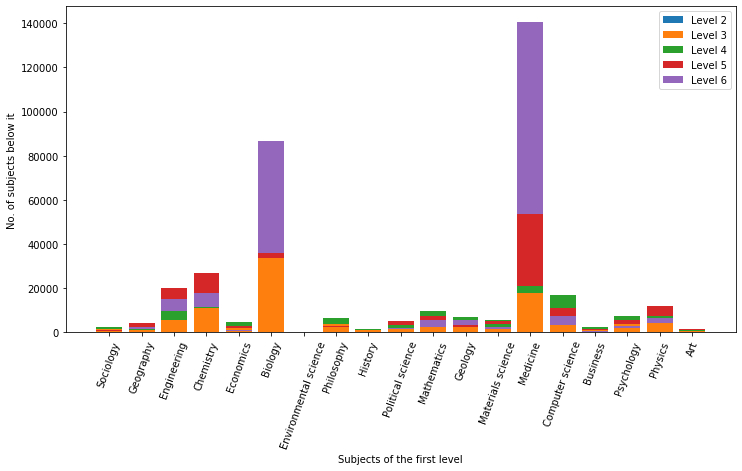
\includegraphics[width=\textwidth]{figures/related_work/makg/subjects_per_field_per_level.png}
    \caption{Subjects present in the MAKG.}
    \label{fig:subjects_per_field_per_level}
\end{figure}

\begin{figure}
    \centering
    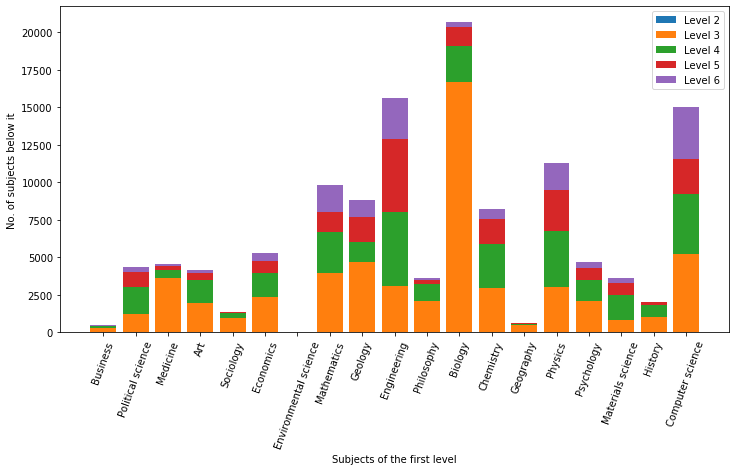
\includegraphics[width=\textwidth]{figures/related_work/makg/subjects_w_article.png}
    \caption{Subjects of the MAKG that have a Wikipedia link.}
    \label{fig:subjects_w_article}
\end{figure}

\begin{figure}
    \centering
    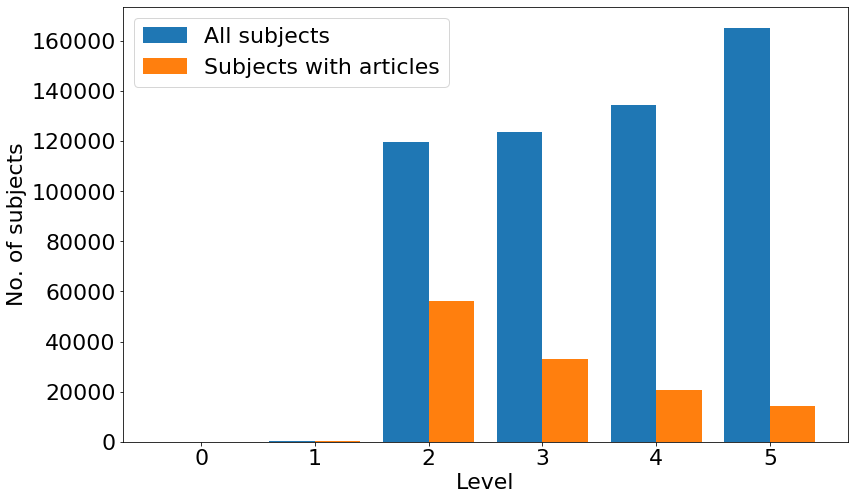
\includegraphics[width=.75\textwidth]{figures/related_work/makg/subject_distribution_comparison.png}
    \caption{Comparison of all subjects with the subset that have a Wikipedia link.}
    \label{fig:subject_distribution_comparison}
\end{figure}

124,385 subjects (17 \% of all subjects) have a Wikipedia link. These are shown in figure \ref{fig:subjects_w_article}. They are relevant for computing the vector representations of the subjects. If they are not present, we cannot do so, as we don't have a text associated to the subject we can use for the vectorization procedure. Biology is the field with the most links, followed by Computer Science and Engineering. Only 4,574 subjects of the 179,741 in the field of Medicine (2.5 \%) have a link, which is why this field is no longer the most populated field when considering Wikipedia links. The difference among all subjects and those with links is shown in figure \ref{fig:subject_distribution_comparison} on a per-level basis. When looking at all subjects, the number increases with the level. When looking at the subjects with links, the opposite occurs: the number of subject decreases with the level.

Regarding the subject assignments of the documents, Färbers files don't include all the subjects assigned to each document. When querying the SPARQL endpoint for all subjects that have been assigned to at least one paper, only 19 subjects are returned. They are very broad subjects, such as \textit{Geology} or \textit{Computer Science}. The assigned subjects in Färbers \acrshort{rdf} files also don't always coincide with the ones assigned by Microsoft. For example, in the \acrshort{rdf} files the paper \textit{Determination of vitamin D3 and 25-hydroxyvitamin D3 in foodstuffs by HPLC UV-DAD and LC–MS/MS} has the subject \textit{Environmental Science}, whereas in Microsoft Academic the topics assigned to the publication include \textit{Vitamin}, \textit{High-performance liquid chromatography} and eight others. These subjects can be retrieved through the \acrshort{api}.
\paragraph{OpenAlex} \mbox{}

OpenAlex\footnote{\url{https://openalex.org/about}} is the successor of the \acrshort{mag}. It offers the whole \acrshort{mag}, combined with several other sources, through a RESTful \acrshort{api}. It arose because the \acrshort{mag} was shut down by Microsoft at the end of 2021, which opened the door for other companies to fill the gap. OpenAlex is still on beta release, which they plan to emerge from in the upcoming months. However, it currently has all the data that \acrshort{mag} had, and more. It also imports data from sources like Crossref\footnote{\url{https://www.crossref.org/}}, ORCID\footnote{https://orcid.org/} and PubMed\footnote{https://pubmed.ncbi.nlm.nih.gov/}.

Among numerous interesting features, it allows searching for publications that are assigned a certain subject. When retrieved from the API, subjects includes the \acrshort{api} request to retrieve its corresponding publications, as well as the number of publications it is assigned to. We can use this number to assess the relevance of a subject. Subjects also include a list with all its ancestors, which we can use to navigate the hierarchy. The \acrshort{api} offers several filters when querying subjects, such as hierarchy level and ancestors.
\paragraph{Choice of data source} \mbox{}

The two options, \acrshort{makg} and OpenAlex, offer different services. \acrshort{makg} stores the \acrshort{mag} data as \acrshort{rdf} triples, which are suited for exploring the knowledge graph through its entities, integrating the \acrshort{mag} data with other sources and performing large scale data analysis \cite{faerber2019microsoft}. OpenAlex, on the other hand, offers a variety of filters to construct granular \acrshort{api} requests, which makes the data very accessible. However, it is not as scalable as the \acrshort{makg}, which can be navigated efficiently with SPARQL.

The main drawback of \acrshort{makg}, which renders it useless for our use case, is that it does not include the assignments of subjects to documents. It only includes the assignment of publications. We require these assignments to build a dataset of documents and their assigned subjects, which we then use to train a supervised classifier. OpenAlex does offer all the assignments that are present in \acrshort{mag}, and therefore is our choice as the data source for subjects and training data. Given that we only require basic filtering and don't want to perform any large scale analysis, we do not require the scalability that \acrshort{rdf} triples offer. The \acrshort{api} objects that OpenAlex outputs fulfill all our requirements.



\section{Related work on supervised approaches} \label{hmc}

In this chapter, we present the relevant literature regarding supervised approaches to \acrfull{si}. We focus on the literature regarding \acrfull{hmc}, a problem in machine learning where objects can be assigned an arbitrary number of labels, and where the labels form a hierarchy. It is a specific case of the \acrfull{mlc} problem. The models are trained by feeding them labeled data, which in our case are assignments of subjects to documents.

\acrshort{hmc} has applications in various disciplines other than \acrfull{nlp}, such as in computer vision, for object recognition tasks, or in biomedicine for predicting the function of proteins. Given the popularity in research of these two disciplines, there is a lot of literature regarding \acrshort{hmc}. We start this chapter by introducing \acrshort{hmc}, including its different approaches. We then go over several neural network architectures that we deem suitable for our use case, and present the relevant literature for each of them.

Binary classifiers are not suitable for our use case because our number of subjects is too high: training 2,157 independent binary classifiers would be computationally expensive. We therefore focus on approaches that comprise only one model, which is responsible for computing the assignment probabilities of all subjects. Convolutional models are well suited for our task because of their feature extraction capabilities. We have found such a model in the literature (\cite{gargiulo2019deep}) that is applied to a similar use case. It will be the basis of our implementation. This model is presented in section \ref{hmc_gargiulo}

We will extend the model in two ways. First, we modify the loss function to account for the imbalance between positive and negative labels in multi-label settings \cite{ben2020asymmetric}, as explained in section \ref{hmc_asl}. The second extension is the implementation of the current \acrshort{sota} in \acrshort{hmc}, which only involves adding a layer on top of the model and again modifying the loss function. This extension ensures that the assignment probability output by the model for each subject is at least as high as the probabilities of its descendants in the hierarchy \cite{giunchiglia2020coherent}. The details of this implementation are shown in section \ref{hmc_forward}.

We also present an application of recurrent networks to \acrshort{hmc}. The recurrence is applied to the levels of the subject hierarchy, which increases the efficiency of the model because of the shared weights \cite{wehrmann2018hierarchical}. However, we discard implementing them, as the authors of the recurrent network show in their experiments that it performs worse than the analogous feed-forward network where the weights are not shared across levels.

\subsection{Introduction} \label{problem_intro}

As discussed in chapter \ref{repo_analysis}, the subjects that are currently present in the repositories are not well maintained. 81 \% of all subjects occur only once, i.e. they are only used by one publication. These cannot be used to relate documents. Furthermore, only 5 \% of the subjects are used by more than 3 publications. The poor quality of the subjects decreases the accessibility of the repositories. Each of them contains thousands of documents, and navigating them can be a cumbersome task. Subjects can be a useful tool for finding the desired documents, and also for looking for documents that are related to the ones we are currently reading.

Consider a repository where there is a maintained set of subjects. Each document in the repository is assigned a subset of these subjects, which can be navigated through the document's page in the repository. If a user is currently reading a publication about brain-computer interfacing, and would like to read more about that topic, the user could browse other documents that handle it by clicking on the corresponding subject. Furthermore, if the user has trouble understanding one of the building blocks of the documents, the user can click on the corresponding subject to search for other documents that maybe present that concept in more detail.
\subsection{Binary classifiers}

Binary classifiers address the data imbalance, which results in poor performance down the hierarchy because of lack of training data, by being optimized individually for each label \cite{banerjee2019hierarchical}. However, multi-label scenarios are usually full of dependencies among labels, which independent binary classifiers do not take into account \cite{liu2017deep}. Furthermore, a collection of binary classifiers is only an option when the number of labels doesn't exceed a few hundreds \cite{banerjee2019hierarchical}. This approach is therefore not interesting for our use case, where there are thousands of labels.
\subsection{Convolutional networks} \label{hmc_cnn}

Convolutions were originally designed for image. However, they can also be used on text, to reduce the size of the data while keeping relevant information. Doing so helps with regularization, as the complexity of the data is reduced. \cite{kim2014convolutional} proposed one-dimensional convolutions and pooling for text input, which are now the common approach. We present these operations here, before discussing two relevant implementations of convolutions for \acrshort{hmc} tasks.

\subsubsection{Convolutions for text}

When applied to text, convolutions are usually one-dimensional. In contrast, convolutions are two-dimensional when applied to images. This has to do with the structure of text and images. The words in a text are ordered across one dimension, whereas the pixels of an image are located in a two-dimensional space. Convolutions extract features from multiple word vectors at a time. Therefore, the result doesn't necessarily change the number of vectors; it affects the number of dimensions.

The number of filters is the number of features we want to extract from each word vector, when considering its surroundings. How large the considered context is, is defined by the kernel size. The number of vectors can be ensured to remain constant with padding, which is done in the original implementation. A single convolution receives $k$ one-dimensional vectors of size $n$ and outputs a single one-dimensional vector of size $m$. $k$ is the kernel size, which defines how many words are considered by each convolution, and $m$ is the number of filters (what PyTorch refers to as output channels), which defines how many vectors remain after the convolutional layer.

\subsubsection{Pooling for text}

Pooling is used to reduce the size of the data while keeping the most important information. The original implementation uses the most popular form of pooling, called max-pooling. Max-pooling takes the maximum over each dimension of the data, thus reducing the number of word vectors. Recall that each dimension represents a feature. The kernel size of the pooling layer defines how many word vectors are considered at a time. For instance, if the kernel size is two, the number of vectors is halved, as the maximum value for all dimensions of each pair of word vectors is kept.

\subsubsection{CNN for HMC} \label{hmc_gargiulo}

\cite{gargiulo2019deep} uses a convolutional model and various embedding methods to index medical documents with MeSH subjects, a hierarchical set of 27,775 subjects regarding Medicine and Biology. Their dataset consists of over eleven million documents from PubMed.

Their architecture comprises three stages. In the first stage, the words are replaced by vectors. The authors try different embedding methods, including the pre-trained fasttext vectors and a normalization pipeline that lower-cased and tokenized the texts, as well as removing numbers punctuation signs, numbers and stopwords. The remaining words were then lemmatized. This is not really an embedding method, but does play an important role in the quality of the embeddings. They experimented with five different embedding methods and various combinations of them. They concluded that the normalization pipeline significantly increased the performance of the model, whereas concatenating different embeddings usually decreased the model's accuracy.

The second stage of their architecture, termed \textit{feature extraction module}, consists of two convolutional layers, followed by max-pooling layers, which reduce the dimensionality of the data while hopefully retaining as much information as possible. A dropout layer with 1 \% discard probability ends this stage, as a regularization method. Interestingly, their first max-pooling layer is said to have size 1, meaning that the maximum value is picked for each window of size 1. This of course is useless; the input to the layer is forwarded without any modifications. We have looked in related work for an explanation, but unfortunately couldn't find any. A previous paper of the first author shows a similar convolutional architecture, but where the max-pooling layer has size 2. This is also the case for the second max-pooling layer in this architecture.

The third and final stage of their architecture is where the indexing occurs. It comprises two fully connected layers, where the size of the output layer equals the number of labels. The first layer has a Rectified Linear Unit (ReLU) activation function and the second, a sigmoid function. The second and third stages, which are the actual neural network model, are depicted in figure \ref{fig:gargiulo}. The first convolutional layer receives a matrix with $N$ words, each of $D$ dimensions. The authors chose 400 as the number of words, padding documents with less words and truncating those with more.

\begin{figure}
    \centering
    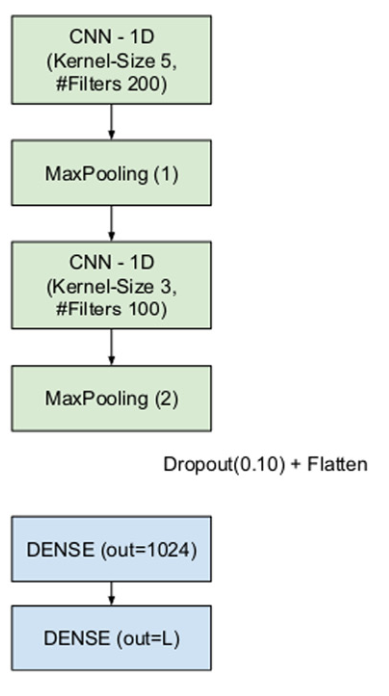
\includegraphics[width=.3\textwidth]{figures/hmc/gargiulo.png}
    \caption{Convolutional architecture for HMC from \cite{gargiulo2019deep}.}
    \label{fig:gargiulo}
\end{figure}

The model is trained with the \acrfull{bce} loss function, which is often used in multi-label settings because each label is treated independently. The model is trained with \acrfull{sgd}, with a mini-batch size of 10, momentum 0.9 and Nesterov accelerated gradients. Besides the comparison of embedding methods, their contribution includes a regularization method, called Hierarchical Label Set Expansion (HLSE), which ensures that if a subject is assigned to a document, its parents are assigned as well. This regularization method reduces the noise in the data, but also increases the complexity of the task, as more labels have to be predicted. However, their experiments conclude that HLSE does increase model accuracy.

\subsection{Feed-forward networks}  \label{hmc_forward}

Feed-forward neural networks are formed by nodes that are connected as a directed acyclic graph (DAG), meaning that there are no cycles. Multi-layer perceptrons, the first kind of neural networks to arise, are a kind of feed-forward networks, where the layers have threshold activation.

\subsubsection{HMC Networks}

\cite{wehrmann2018hierarchical} presents a feed-forward architecture that outperforms previous \acrshort{hmc} approaches for a variety of use cases and datasets. The network comprises one layer per level in the subject hierarchy, each outputting its own local loss. These losses are then added to the global loss, after being weighted. How important local losses are is case-dependent. Therefore, the weight parameter can be adjusted.

Each layer also receives the original input, as shown in figure \ref{fig:hmcn-f}. This allows each layer to associate features from the input to the classes of the hierarchy level it represents. Thus, a layer learns features for a specific level of the subject hierarchy by processing both the original input and the output of the previous layer, i.e. the previous level of the hierarchy. According to the authors, introducing local losses feeds the network with specific local information that would otherwise be ignored, and prevents dead neurons (i.e. neurons with weight and bias close to zero) because of the increased gradient signal, which also accelerates convergence.

As is common in the multi-label setting, the authors have also picked binary cross-entropy as the loss function. Training is controlled by the Adam optimizer and a learning rate of $10^{-3}$. They used ReLU activation functions for all hidden neurons and sigmoid for the output neurons. Batches are normalized and their parameters are dropped out with a probability of 60 \% to avoid overfitting.

\begin{figure}
    \centering
    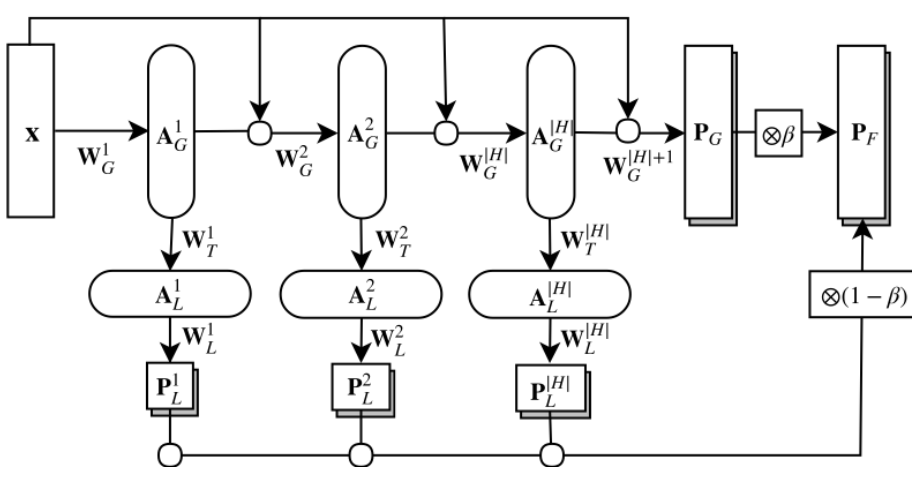
\includegraphics[width=.8\textwidth]{figures/hmc/hmcn-f.png}
    \caption{Architecture of the feed-forward HMC network from \cite{wehrmann2018hierarchical}.}
    \label{fig:hmcn-f}
\end{figure}

\subsubsection{Coherent HMC Networks}

Another feed-forward architecture was proposed in \cite{giunchiglia2020coherent}, which outperformed the architecture presented above in 17 out of 20 datasets, with a much simpler architecture. Instead of introducing local losses for the levels of the hierarchy, this approach enforces the hierarchy on the assignment probabilities by modifying the probabilities of subjects if one of their descendants has higher probability.

For example, if a document is assigned the subject \textit{k-nearest neighbors} with probability $0.7$, the probability of \textit{clustering algorithms} should at least be $0.7$. The authors ensure this is the case by picking for each class the maximum probability between its own probability and the probabilities of its descendants in the hierarchy. Formally, they introduce this constraint in the architecture with an additional layer called \acrfull{mcm}, which, for each subject, picks the maximum probability between its own and that of its descendants. Given a subject $A$ and its descendant $B$, for which a model outputs probabilities $p_A$ and $p_B$, the \acrshort{mcm} outputs the following probabilities for each node:

\begin{align*} 
    & MCM_B = p_B \\ 
    & MCM_A = \max(p_A, MCM_B)
\end{align*}

Their second contribution is a modification of the \acrfull{bce} loss function, which doesn't take into account the dependencies between labels. Their loss function incentivizes the model to respect the subject hierarchy, i.e. that subjects should not be assigned probabilities lower than the probabilities of its descendants. This loss function, called \acrfull{mcl}, can be defined for the two nodes $A$ and $B$ described above as follows:

\begin{align*} 
    & MCL_B = -y_B \ln(MCM_B) - (1 - y_B) \ln(1 - MCM_B) \\ 
    & MCL_A = -y_A \ln(\max(p_A, p_B \cdot y_B)) - (1 - y_A) \ln(1 - MCM_A)
\end{align*}

The loss for the descendant subject $B$ is computed exactly as in the \acrshort{bce} loss function, using $MCM_B$ instead of the model's output $p_B$. Note that $y_A, y_B \in {0, 1}$ are the true labels of the subjects $A$ and $B$ for a given document. The loss for the ancestor subject $A$ differs from the \acrshort{bce} loss in that in the first logarithmic term. In fact, it only changes when the subject $B$ should be assigned to the document (i.e. $y_b = 1$). Then, the loss of its ancestor $A$ takes the max function takes the maximum between $p_A$ and $p_B$ for the first logarithmic term of its loss.

For example, if the descendant subject $B$ had a higher probability than its ancestor $A$ in the model output ($p_B > p_A$) and only $A$ should be assigned to the document ($y_A = 1, y_B = 0$), the \acrshort{bce} loss would wrongly output that $p_B$ should be increased and $p_A$ kept as is. MCL, on the other hand, outputs the right losses, stating that $p_A$ should be increased and $p_B$ decreased, so the hierarchy is not violated.
\subsection{Recurrent networks}

Recurrent neural networks are similar to feed-forward networks, but their nodes do form a cycle, This allows them to exhibit temporal behavior, i.e. they can handle sequential data. They are also characterized by their efficiency, as weights are shared across the layers (which are iterations in the presence of recurrence), making recurrent networks much smaller than feed-forwad networks.

\subsubsection{HMC Networks}

\cite{wehrmann2018hierarchical}, whose feed-forward network we presented above, also proposes a recurrent architecture. The feed-forward architecture already resembles a recurrent network, with each layer having its own input and output, while being sequentially communicated with other layers. Therefore, modifying it to be recurrent is straight forward. Doing so also addresses an issue of the feed-forward network, namely that the number of parameters increases with the number of hierarchy levels. Recurrent networks share weights across layers, therefore having a constant number of weights, regardless of the number of levels in the hierarchy.

The authors used a Long Short-Term Memory (LSTM) architecture for their recurrent network, which already regulates the gradient and thus prevents it from vanishing during the backward pass. The recurrent network was slightly worse than the feed-forward one, but is much smaller in terms of parameters. In one of their experiments, the feed-forward architecture had seven million parameters, whereas the recurrent network had three million. The authors recommend using the recurrent network for hierarchies with many levels, as in such cases the difference in size between the architectures is larger and the minimal gain in performance is not worth the additional complexity.
\subsection{Asymmetric loss function} \label{hmc_asl}

\cite{ben2020asymmetric} addresses the imbalance between positive and negative labels in multi-label settings with an \acrfull{asl} function that dynamically down-weights and hard-thresholds easy negative samples, while also discarding possibly mislabeled samples. Training the state-of-the-art models in computer vision with this loss function significantly outperforms previous methods. On ResNet101, the common architecture used for multi-label classification, the asymmetric loss improves previous results by more than 1 \%. The \acrshort{asl} is also popular for its robustness against noise, as it is better suited for modeling noise in \acrshort{mlc} settings \cite{zhao2021evaluating}. The choice of the loss function plays a key role on how the model handles noise \cite{karimi2020deep}.

\subsubsection{BCE and focal loss}

\acrfull{bce}, the most popular loss function in multi-label classification settings, treats every label the same. For example, in a one-label setting where the model outputs $p=0.7$, if the label is positive ($y=1$), the \acrshort{bce} loss would be $-log(0.7) = 0.4$. If negative ($y=0$), the \acrshort{bce} loss would be $-log(0.3) = 1.2$, i.e. larger than in the other case, as the predicted probability is further away from the true label. The problem with using \acrshort{bce} in a multi-label setting is that most of the true labels for any given input are usually negative. In our case, any document is assigned only a few of the available subjects.

$$ BCE = \frac{1}{K} \sum_{k=1}^K -y_k \cdot \log (p_k) - (1-y_k) \cdot \log (1-p_k) $$

\acrfull{fl} addresses this issue by weighting each label score in a way that model outputs that are further away from their true labels gain more importance, whereas the model outputs that are already close to their targets are weighted down. Returning to the previous example and setting $\gamma=1$, a model output of $0.7$ with a positive true label ($y=1$) would receive a \acrshort{fl} of $-0.3 \cdot log(0.7) = 0.1$, and with a negative label ($y=0$), the \acrshort{fl} would be $-0.7 \cdot log(0.3) = 0.8$.

If we compare the results of both losses, we see that the difference between the results is much larger when using the \acrshort{fl}: they differ by a factor of 8 instead of by a factor of 3. The \acrshort{fl} gives more importance to the model output that was far away from its true label. Thus, the higher the \acrshort{fl} parameter $\gamma$ is set, the larger the difference will be between outputs that are close to their labels and those that are further away. However, setting $\gamma$ too high could remove the gradients from the rare positive samples \cite{ben2020asymmetric}.

$$ FL_\gamma = \frac{1}{K} \sum_{k=1}^K -y_k \cdot (1-p_k)^\gamma \cdot \log (p_k) - (1-y_k)\cdot p_k^\gamma \cdot \log (1-p_k) $$

\subsubsection{Asymmetric loss}

\acrfull{asl} overcomes this issue by decoupling the $\gamma$ parameter for negative and positive true labels, i.e. into $\gamma_-$ and $\gamma_+$, respectively. Setting $\gamma_- > \gamma_+$ emphasizes the contribution of positive samples, while giving less importance to negative samples that are close to their true label. Each of these three loss functions is an extension of the previous one. \acrshort{fl} equals \acrshort{bce} for $\gamma=0$, and \acrshort{asl} equals \acrshort{fl} for $\gamma_- = \gamma_+$.

$$ ASL_{\gamma_-,\gamma_+} = \frac{1}{K} \sum_{k=1}^K -y_k \cdot (1-p_k)^{\gamma_+} \cdot \log (p_k) - (1-y_k)\cdot p_k^{\gamma_-} \cdot \log (1-p_k) $$

The authors also propose using a hard threshold to discard negative samples below it, to further direct the training towards the positive samples. Although improving the performance of the models, this addition increases the complexity of the model, adding another parameter that requires tuning. They also experimented with dynamically tuning the $\gamma$ values, but concluded that doing so hindered the performance of the models. Still, they state this scheme could be useful for novice users.
\section{Unsupervised approach} \label{unsupervised_approach}

Here we present our first approach. It is inspired by the \acrfull{si} procedure performed by Microsoft to create the \acrfull{mag}, as outlined in a demo paper \cite{shen2018web}. We use the subjects they have discovered, as well as the hierarchy they extracted from the assignments. Details on their implementation can be found in section \ref{subject_indexing_mag}. Our goal is not to compare our results with Microsoft's, nor to fully reproduce their approach. Rather, our intention is to implement a fully unsupervised procedure, which doesn't depend on any external sources of data. We also require our implementation to be simple.

We have built a vocabulary based on the relevant documents of the repositories. At first, it contains all lemmatized tokens of the repositories. We then remove the tokens that appear in only one document, to reduce the size of the vocabulary. The details of the vocabulary construction can be found in section \ref{implementation_vocab}. We then train the embeddings of the vocabulary entries with the skip-gram model. The resulting vectors are used to vectorize documents and subjects, which are then compared in vector space regarding their similarity. In section \ref{implementation_skipgram}, we show the results of the training procedure and offer some examples.

We enrich the representation of documents by adding the representations of other documents that appear under the same venue, advisor and referee in the repositories. They handle similar topics, and therefore improve the representation of each other. Subjects, on the other hand, are enriched with text from their corresponding Wikipedia articles. We finally sort the words of each representation by frequency, removing duplicates. In section \ref{unsupervised_approach_representations}, we explain thoroughly how documents, subjects and venues are represented.

The representations of documents and subjects are then vectorized with the word embeddings. We compare them in vector space regarding the similarity, to find the subjects that should be assigned to each document. We have developed three methods to compute similarities, which we present in section \ref{unsupervised_approach_vectorization}, together with some examples that illustrate how they work. Adding together the word vectors of each representation seems to offer the best result. This will be properly tested in the evaluation (chapter \ref{eval}).

Finally, in section \ref{unsupervised_approach_conclusion}, we analyze the procedure, looking for decisive factors and possible improvements. The implementation is tedious, as it comprises many steps and details. Its accuracy can be increased by improving the vocabulary by discarding uninformative words and adding relevant phrases. Experimenting with other ways of representing texts, such as keeping duplicates, may also be beneficial.

\subsection{Building the vocabulary} \label{implementation_vocab}

The first step of the implementation is building the vocabulary. Words that are not included in it will be discarded when computing the vector representations for the documents, venues and subjects. Therefore, it is a very important step. It should include all words  that are relevant for the task of \acrshort{si}, i.e. the words that describe the topics each document handles.

The vocabulary is directly extracted from the corpus (the titles and abstracts of the documents). Only words that appear in the documents can be present in the vocabulary. There are several design choices that should be considered. We use SpaCy's small trained pipeline (called ``en\_core\_web\_sm'') for tokenization. The lemmatization is performed by the WordNet lemmatizer of NLTK, using the \acrfull{pos} tags computed by Flair's sequence tagger. The reasoning behind these choices are discussed in the following sections.

\subsubsection{Tokenizer}

Tokens are the semantic units that \acrfull{nlp} pipelines build upon. They are usually words, but depending on the task at hand, one can tokenize strings in different ways. For example, \textit{aren't} can be kept as a token or divided into two tokens, \textit{are} and \textit{n't}. This kind of decisions are made by the tokenizer, an algorithm that divides a given text into tokens. Tokenizers are usually based on simple heuristics.

We use the tokenizer from spaCy\footnote{\url{https://spacy.io/usage/linguistic-features\#how-tokenizer-works}}. It tokenizes words (which are surrounded by white spaces) by iteratively looking for prefixes and suffixes until a match is found with a regular expression that defines how a token should look like. Another reason why we pick this tokenizer is because it is included in Flair \cite{akbik2019flair}, an \acrshort{nlp} framework which we use later on to compute the \acrshort{pos} tags of each token.

\subsubsection{N-grams} \label{vocab_ngrams}

In some cases, words pose different meanings when combined with others. For example, ``ice cream'' has a particular meaning, and it should therefore be present in the vocabulary as a phrase. The words ``ice'' and ``cream'' pose different meanings when used independently. Such phrases also occur in the scientific jargon. For instance, ``machine learning'' refers to a field of computer science, something that cannot be deduced from its name. Still, the name describes well the purpose of the field (teaching machines how to learn). This is usually the case with scientific terms: they aim to describe their application as clearly as possible.

We built a vocabulary with n-grams of up to length four, to see its size and constituent entries. After filtering out the ones that appeared in only one document and those that appear in more than 1,000 documents, we found out that the n-grams weren't as informative as we expected. Many of them were just common sequences of words, such as ``this is a problem''. We talk about this vocabulary in detail in the appendix. We decided against including n-grams because the increase in quality was low compared with the increase in computational cost. 

\subsubsection{Vocabulary normalization}

The purpose of normalizing a vocabulary is to reduce its size by grouping words with similar meanings together. We will now introduce two normalization techniques that we have included in our procedure: case folding and lemmatization.

\paragraph{Case folding} \mbox{}

The most straight-forward way of reducing the size of the vocabulary is case folding. For example, the word ``here'' may be capitalized because it is at the beginning of the sentence and would thus appear as another entry in the vocabulary. Writing all words in lower case eliminates this duplicity issue.

Case folding is not suitable for tasks where proper nouns should be identified. For example, the word ``frank'' has a different meaning than the name ``Frank''. This issue is not relevant for our task, as we are mainly interested in scientific words that have unique meanings. Therefore, we perform case folding on all words before adding them to the vocabulary.

\paragraph{Lemmatization} \mbox{}

Lemmatization consists of replacing words by their semantic roots. It makes the model more general by removing verb conjugations, plural cases and other variations of words that ultimately have the same meaning. This technique may also reduce the precision of the model. For instance, words with different meanings, such as ``bank`` and ``banking'', are reduced to the same lemma even if the meaning of the word ``bank'' is context-dependent. Such situations are a priori not dangerous for our task, as scientific words usually have concise meanings.

Stemming is a similar approach, in which prefixes and suffixes are removed. For example, the stem of the word ``house'' is ``hous'' and its lemma is ``house''. Lemmatization is more accurate because it takes into account the meaning of the word \cite{hapke2019natural}. A good example of this is ``better'', whose lemma is ``good'' while its stem is ``bet'', which has a completely different meaning. Because of this, lemmatizers are suitable for more applications, and ours is no exception.

We use the WordNet lemmatizer of the NLTK package in our pipeline. WordNet \cite{fellbaum2010wordnet} is a lexical database that is publicly available and offers lemmatization. NLTK provides an interface to this lemmatizer. The accuracy of the lemmatization improves when the \acrfull{pos} tag of the word that should be lemmatized is also provided. We do so using the fast universal \acrshort{pos} tagger from Flair \cite{akbik2019flair}, called ``upos-fast''. The model, which combines Flair's contextual word embeddings \cite{akbik2018contextual} with a LSTM-CRF model, is trained on the data set of the CoNLL's shared task of 2018 \cite{zeman2018conll}, which comprises words in 12 languages. The resulting tagger has an F1-score of 98.47\footnote{As seen here (accessed on 06.07.2021): \url{https://github.com/flairNLP/flair/blob/master/resources/docs/TUTORIAL_2_TAGGING.md}} on the Ontonotes data set, only behind its larger version, called ``upos''. The difference between them is too small (0.13) to account for the large difference in performance. Using the faster model speeds up the procedure by around 500 \%.

\subsubsection{Vocabulary filtering} \label{vocab_filtering}

Once the vocabulary has been created, we remove the entries that occur in only one document, as their meanings may be too specific to relate documents to one another. Entries that are either stop words\footnote{For this purpose, we use NLTK's list of English stop words, which comprises 179 words as of 07/07/2021.} or punctuation signs are also discarded. Symbols such as Greek letters are kept, as they refer to certain concepts in fields like Physics or Mathematics.

At first, we discarded entries that occur in more than 1,000 documents, which reduced the size of the vocabulary to 49,651 entries. However, this also resulted in 7,188 documents not having any words that were in the vocabulary, meaning that they could not be vectorized. Given that there are only 488 vocabulary entries that occur in more than 1,000 documents, we decided to keep them. This greatly improves the coverage: now only 85 documents cannot be represented.

\subsubsection{Resulting vocabulary} \label{vocab_results}

In our corpus, there are 125,575 distinct tokens. 75,436 of them appear in only one document and are discarded. Thus, the final vocabulary comprises 50,139 entries. With this vocabulary, only 85 documents cannot be represented, i.e. none of the words of their titles and abstracts appear on the vocabulary. Keep in mind that 51 of those documents didn't have any texts to begin with, as stated in section \ref{repo_analysis_data}.

In figure \ref{fig:bow_data}, the number of tokens of the documents that are included in the vocabulary is displayed. As mentioned before, 85 documents don't have any of their tokens in the vocabulary. 110 have just one. On the other end of the spectrum, 24,819 documents have nine or more tokens in the vocabulary. This accounts for 84 \% of all documents. Vocabulary entries appear on average on 27.1 documents. Figure \ref{fig:vocab_1grams} shows in how many documents each entry of the vocabulary occurs, grouped in bins. 46,776 entries (94 \%) appear in 100 documents or fewer. 15,250 entries (31 \%) appear in only two documents.

\begin{figure}
    \centering
    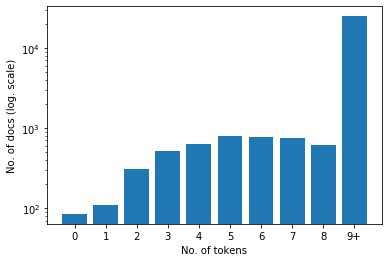
\includegraphics[width=.7\textwidth]{figures/unsupervised_approach/bow_data.png}
    \caption{Distribution of the documents depending on the number of their tokens that are included in the vocabulary.}
    \label{fig:bow_data}
\end{figure}

\begin{figure}
    \centering
    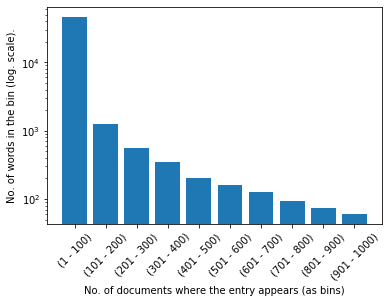
\includegraphics[width=.7\textwidth]{figures/vocab/vocab_1grams.png}
    \caption{Distribution of the vocabulary entries depending on the no. of documents they are included in.}
    \label{fig:vocab_1grams}
\end{figure}
\subsection{Embedding model} \label{implementation_skipgram}

To transform text into vectors, we first embed words into vector space. We could do so randomly, but this wouldn't take into account the semantic information of the words. To preserve this information, we use skip-gram \cite{mikolov2013distributed}, a word embedding model. This model was also used by \acrshort{mag} in their procedure. We already gave an overview of its design in section \ref{mag_skipgram}. In this section, we will look at how we trained the model and some examples of the resulting embeddings.

We train 100-dimensional word vectors, which we initialize with values sampled from the uniform distribution bounded by -1 and 1. The word vectors of \acrshort{mag} comprise 250 dimensions. We have decided to use fewer dimensions given that our vocabulary is much smaller: it includes around 50,000 entries, whereas \acrshort{mag}'s vocabulary has than 2 million.

We trained the model for 8 epochs. Surprisingly, it reached its best epoch loss already in the second iteration. The model optimized the embeddings quickly during the first epoch, starting with a batch loss of $30$ and ending with an average epoch loss of $4.9$. Figure \ref{fig:loss_avgs} shows the avg. loss of each epoch. Figure \ref{fig:loss_avgs_range} also shows the avg. loss, but with bars illustrating the range of the batch losses throughout the epoch.

\begin{figure}
  \begin{subfigure}[t]{0.5\textwidth}
    \centering
    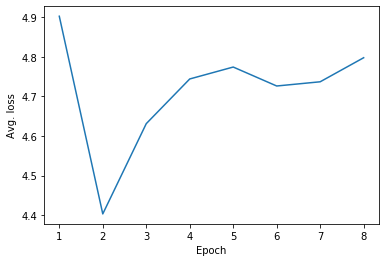
\includegraphics[width=\textwidth]{figures/unsupervised_approach/loss_avgs.png}
    \caption{Avg. training loss of each epoch.}
    \label{fig:loss_avgs}
  \end{subfigure}
  \hfill
  \begin{subfigure}[t]{0.5\textwidth}
    \centering
    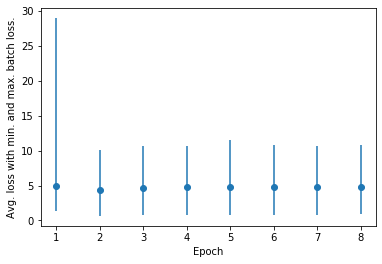
\includegraphics[width=\textwidth]{figures/unsupervised_approach/loss_avgs_range.png}
    \caption{The dots refer to the avg. epoch loss, while the extrema of the line refer to the min. and max. batch loss of that epoch.}
    \label{fig:loss_avgs_range}
  \end{subfigure}
  \caption{Plots of the training loss of the skip-gram model.}
\end{figure}


\subsubsection{Resulting embeddings}

We have computed the cosine distance between certain words to serve as an example. The cosine distance is also the metric we use to compare subjects and documents. The results can be found in table \ref{tab:embeddings_examples}. We have chosen three pairs of words, each of a different field. `polymer'' and ``monomer'' belong to the realm of chemistry; ``machine'' and ``learning'' usually refer to a family of algorithms; ``magnetic'' and ``resonance'' refer to a medical procedure. The chemistry pair is fed to the skip-gram model 96 times during training; the computer science pair, 1357 times and the medicine pair, 961 times.

Given that the cosine distance is symmetric, we only show one half of the table. Also, the distance of a vector to itself is zero. The table shows that the pairs of words of each field are closer to each other than to the other words. The distance between ``polymer'' and ``monomer'' is the largest of the three, which makes sense, as the model receives this pair of words hundreds of times less than the two others. The smallest distance between words that do not belong to the same field is between the words ``magnetic'' and ''polymer''. This distance is 34 \% larger than the distance between ``monomer'' and ``polymer''. Thus, the word vectors accurately differentiate between words that belong to the same field and those that don't.

As a further example of the semantic expressiveness of the embeddings, we can look at the word ``program'', although it belongs to the same field as the computer science pair, it is not as closely related to them. In fact, it appears 27 times as an input to the model with either of the words ``machine'' and ``learning''. However, this is more often as for the pairs of chemistry and medicine, with which it appears as input 26 and 3 times, respectively. The model was able to identify that ``program'' should be closer to the computer science pair, even if it appeared only one time less with the chemistry pair. Its cosine distance to ``machine'' and ``learning'' are 0.77 and 0.72, respectively. On the other hand, its cosine distance to the rest of the words is above 1.

\begin{table}[]
    \centering
    \begin{tabular}{c|c c c c c c}
       $dist(x,y)$ & monomer & polymer & machine & learning & magnetic  \\
       \hline
       resonance & 0.96 & 0.91 & 0.95 & 0.95 & \textbf{0.21} & \\
       magnetic & 0.88 & 0.82 & 0.98 & 0.98 & & \\
       learning & 1.08 & 1.19 & \textbf{0.41} & & & \\
       machine & 1.02 & 0.95 & & & & \\
       polymer & \textbf{0.54} & & & & & \\
    \end{tabular}
    \caption{Cosine distances between the vectors of certain words. The distances of words of the same field are highlighted in bold.}
    \label{tab:embeddings_examples}
\end{table}
\subsection{Vector representations} \label{unsupervised_approach_representations}

In this section, we talk about the vector representations of the three different elements of our corpus (documents, venues and subjects). This procedure is an adaptation of \acrshort{mag}'s approach \cite{shen2018web} to our scenario. An important difference between our setting and that of \acrshort{mag} is that ours includes theses, which are not published in any venue.

In the following three sections we will look at the information used to represent venues, documents and subjects. Each element has both a \acrfull{srt} and an \acrfull{ert}. The \acrshort{srt} consists of basic information of the element, whereas the extended one comprises information of associated elements, which are used to enrich the representation of each element.

\subsubsection{Venues}

Venues are journals, conferences and other organizations where researchers can publish their work. They usually accept publications regarding a certain field, such as the \textit{Journal of Clinical Medicine}, which publishes medical work. Some are even more specific, such as the \textit{International Conference on Dublin Core and Metadata Applications}, which only includes publications that have to do with metadata, an area of computer science. Others are more interdisciplinary, including publications of different fields. An example of such a venue is the \textit{Journal of Chemical Physics}, which is a subdiscipline of both Chemistry and Physics. There are venues that are even more broad, such as the famous \textit{Nature}, which comprises all natural sciences and technology.

Regardless of their scope, venues can be useful to identify what topics their publications revolve around. Therefore, the representations of venues are used in the representations of documents. Specifically, their representations are added, with the venue's representation being weighted down. The venues present in the repositories were already analyzed in section \ref{repo_analysis_venues}. Given that there are many types of venues, they appear under various names in the repositories, such as \textit{Journal title} or \textit{Proceedings}. How venues are stored also differs between repositories.

An important difference between our use case and \acrshort{mag}'s, is that we also consider theses, which are not published in any venue. We argue that advisors and referees have a similar role for theses as venues have for publications. We therefore use them as a replacement for venues when considering theses. We then look at how \acrshort{mag} computes the \acrshort{ert}s of venues, and how we do so in our use case. In the end, venues are represented by a sample of the documents they are assigned to, whose representations are concatenated.

\paragraph{Alternative venues for theses} \mbox{} \label{unsupervised_approach_venues_theses}

Given that 36 \% of our documents are theses and thus were not published anywhere, we require a workaround that allows for theses to also be grouped by the topics they handle. If we didn't find an alternative, the representations of theses would be considerably less precise than those of publications, which would hamper the quality of the \acrshort{si}. Just as venues publish research work that handles the topics they focus on, referees and advisors of theses only do so when the topics handled by the student aligns with their fields of expertise. They are therefore good indicators of the semantic content of a thesis.

As discussed in section \ref{repo_analysis_contributors}, theses of edoc and refubium almost always have at least one referee (only 1 \% and 5 \% of the theses don't have one, respectively). On the other hand, 19 \% of the theses of depositonce are missing a referee. The missing referees in depositonce are luckily replaced by advisors. Depositonce is the only repository where advisors appear often. Only 4 \% of the theses there don't have one. Edoc and refubium have almost no advisors.

Given the differences among the repositories, both referees and advisors have to be considered as an alternative for venues when grouping theses. When doing so, only 5 documents of depositonce (0.07 \%) don't have an expert (i.e. neither an advisor nor a referee). 30 documents of edoc (0.4 \%) are also missing an expert, as well as 662 documents of refubium (5 \%). These and other facts are shown in table \ref{tab:experts}, including that, on average, theses feature more than two experts. This may help identify the topics of theses that are multidisciplinary, i.e. whose subjects belong to several fields.

\begin{table}[]
    \centering
    \begin{tabular}{|c|c|c|c|c|}
    \hline
         \thead{Repository} & \thead{No. of \\ experts} & \thead{No. of distinct  \\ experts} & \thead{Avg. no. \\ of experts \\ per thesis} & \thead{No. of theses \\ without \\ an expert} \\
         \hline
         depositonce & 8,383 & 2,338 & 2.6 & 5 (0.07 \%) \\
         \hline
         edoc & 7,308 & 3,395 & 2.8 & 30 (0.4 \%) \\
         \hline
         refubium & 9,133 & 4,863 & 2.2 & 662 (5 \%) \\
         \hline
    \end{tabular}
    \caption{Facts regarding the experts of theses.}
    \label{tab:experts}
\end{table}

\paragraph{Simple representation} \mbox{}

\acrshort{mag} uses the name of the publishing venue as its \acrshort{srt} \cite{shen2018web}. For referees and advisors, we could use the name of the person as its \acrshort{srt}. However, the names of professors have no relationship with their fields of expertise, and therefore would not provide any information about the topics they work on. We therefore discard the names of venues altogether, for the sake of simplicity.

\paragraph{Extended representation} \mbox{}

\begin{figure}
    \centering
    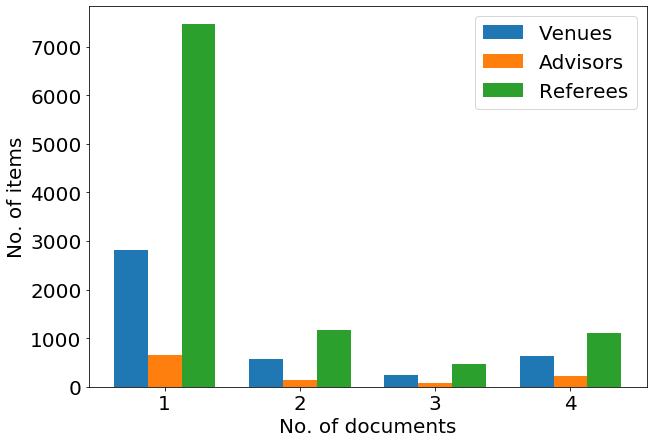
\includegraphics[width=.7\textwidth]{figures/unsupervised_approach/ert_counts.png}
    \caption{No. of documents included in the creation of the ERT of venues, referees and advisors.}
    \label{fig:ert_counts}
\end{figure}

The \acrshort{ert} of a venue is formed by concatenating the \acrshort{srt}s of a sample of its publications. The authors of \acrshort{mag} don't specify how many publications they use for the \acrshort{ert} of each venue. Given that our venues have on average 4.2 publications assigned to them, we pick 4 as the maximum sample size. Venues with less than four documents will take as many documents as there are available to compute their \acrshort{ert}. We do the same for advisors and referees. Those that have more than four documents available are assigned the four longest documents in terms of the number of tokens that are present in the vocabulary, instead of randomly sampling four documents. In this way, we improve their representations by ensuring they comprise as many tokens as possible.

Figure \ref{fig:ert_counts} shows how many documents are used to represent each item (venue, referee or advisor). Most of the items only include one document in their representations. This is the case for 66 \% of the venues, 59 \% of the advisors and 73 \% of the referees. This fact will be important when evaluating the accuracy of our vector representation for the items. Items that include more documents are expected to have more accurate vector representations.

There are six venues and thirteen referees that cannot be represented. Even if they have documents assigned to them, these do not include any tokens that are present in the vocabulary. There are also several more that have only a few tokens on average, as can be seen in figure \ref{fig:bow_venues}. On the other hand, there are only three advisors with less than nine tokens on average. These averages refer to the avg. amount of tokens of their constituent documents, i.e. those that were picked for their \acrshort{ert}.

\begin{figure}
    \centering
    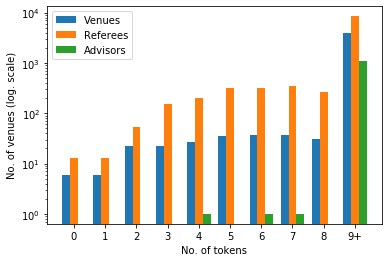
\includegraphics[width=.7\textwidth]{figures/unsupervised_approach/bow_venues.png}
    \caption{Avg. number of tokens of venues, referees and advisors.}
    \label{fig:bow_venues}
\end{figure}

\subsubsection{Documents}

Documents are the publications and theses of the repositories that are written in English. The \acrshort{srt} of a document comprises its title and abstract, and the \acrshort{ert} results from concatenating the \acrshort{ert} of its venue. In this section, we will look at both representations, comparing our implementation with that of \acrshort{mag}. There are some challenges that arise from the small size of our dataset. For instance, the extracted references often pointed to papers outside our dataset, being thus of no use to relate documents to one another.

\paragraph{Simple representation} \mbox{}

Creating the \acrshort{srt} of the documents is straight forward. We can extract the title and the abstract of a document through the OAI-PMH interface of each repository. \acrshort{mag} also uses the keywords, but these are not available in the metadata of the papers. We therefore only use the title and the abstract to represent each document. We cannot use the subjects assigned by the users that uploaded the documents because these will be used to evaluate the performance of our model.

We discard using the full texts of the documents because doing so would complicate the encoding task. Only the most important aspects covered by the paper are included in the abstract, which are the ones we want to consider. Using the full texts could potentially reduce the quality of the encodings, as they cover topics that are not central to the ``aboutness'' of the paper, such as the related work. Furthermore, extracting the texts from the PDFs is time-consuming and computationally expensive.

After processing the texts and removing the tokens that are not included in the vocabulary, documents have on average 37 tokens. 85 documents don't have any, and over 84 \% of them have nine or more tokens. These and some other facts, along with figure \ref{fig:bow_data}, were already discussed in section \ref{vocab_results}, as they were used to determine the size of the vocabulary.

\paragraph{Reference and citation extraction} \mbox{} \label{unsupervised_approach_references}

A reference used by a document $A$ is another document $B$ which the document $A$ uses to lay the foundation of their work. It gives the reader an understanding of the scope of their work, as well as the fields involved. Document $B$ is then cited by document $A$, i.e. citations can be understood as the inverse relations of references: if document $B$ is a reference of document $A$, document $A$ is a citation of document $B$.

To extract the references from the papers, we use a package called \textit{refextract}\footnote{\url{https://github.com/inspirehep/refextract}}. It returns the references it finds in a given text as a dictionary, which includes the title, authors, journal title and other data about each of the referenced papers. Refextract uses regular expressions to identify the elements of the reference, as well as mappings for special cases. It was developed to be used for scientific papers of \textit{High-Energy Physics}\footnote{\url{https://www.energy.gov/science/hep/high-energy-physics}}, an American laboratory. This means that the special cases included in the knowledge bases focus on this specific set of papers. Therefore, we expect the accuracy to be worse in our heterogeneous dataset, which comprises papers written in various formats as well as theses.
 
Using this package, together with a Python port to the Apache Tika library\footnote{\url{https://github.com/chrismattmann/tika-python}} to parse the text from the PDF files, we successfully extracted the references of 29,329 documents. Only 5 documents of depositonce and 14 of refubium didn't have any references. In edoc there are 50 files where no references could be extracted. These documents either did not have any files, the file did not include references, or the format of the references could not be identified.

The documents for which we could extract references, include on average 157 references. This number is so large because of the theses, which on average comprise 246 references. Publications include on average 105 references. This number is so large because of refubium, whose documents include on average 121 references. Edoc and depositonce include 85 and 91 references on average, respectively. Unfortunately, most of these references point to documents outside the repositories. Only 328 documents (1.2 \% of all the documents) refer to other documents in the repositories. They do so an average of six times. The remaining 29,001 documents (99 \% of all documents) cannot be related through their lists of references.

\paragraph{Extended representation} \mbox{}

In \acrshort{mag}, the \acrshort{ert} of a document comprises three different aspects (references, citations and venues). As was just mentioned, the size of our dataset is too small to profit from relations among papers through their lists of references. Therefore, we only use the \acrshort{ert} of its associated venues, referees and advisors. These are added to the \acrshort{srt} after being multiplied with a weighting factor $w$. Here is the equation for computing the \acrshort{ert} of documents:

$$ h_e^d = h_s^d + w \cdot \frac{1}{n} \sum_V h_e^V $$

$h_s^d$ refers to the \acrshort{srt} of a document; $h_e^V$ refers to any venue, advisor or referee that is related to the document. The creators of \acrshort{mag} don't disclose how they weighted venues in the paper. Therefore, we decided to choose $0.7$ as the weight parameter. Our choice is probably higher than the one used in \acrshort{mag}. This makes sense as we have less data available to represent documents.

Once the representations of documents are enriched with the representations of their venues, only 33 documents remain without tokens, out of the 85 that were empty before. The number of tokens per document is illustrated in figure \ref{fig:doc_representations}, which can be compared to figure \ref{fig:bow_data}, where the same data is shown but without including venues. On average, document representations comprise 324 tokens, including tokens of 1.5 venues. 20,399 documents include only one venue, whereas 7,430 documents include either two or three venues. Almost 98 \% of the documents have more than eight tokens in their \acrshort{ert}.

\begin{figure}
    \centering
    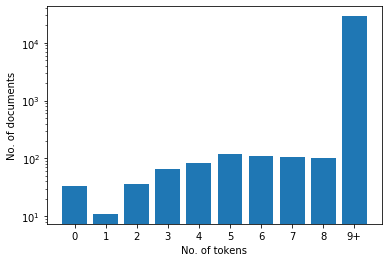
\includegraphics[width=.7\textwidth]{figures/unsupervised_approach/doc_representations.png}
    \caption{Number of tokens in the extended representation of the documents.}
    \label{fig:doc_representations}
\end{figure}

\subsubsection{Subjects}

Subjects are the concepts we use to describe the content of the documents. Each document is assigned a variable number of subjects, which together define what the document is about. We already discussed how subjects were retrieved from OpenAlex in section \ref{problem_scope_subjects}. The resulting set comprises 2,157 subjects, evenly distributed among the 19 fields.

Here, we explain what information we use to describe the subjects. Microsoft performed manual steps to create the \acrshort{ert} of the subjects that we are unable to emulate. Therefore, subjects only comprise a \acrshort{srt}, which is their Wikipedia article. This is the only external information we use throughout this approach, as we have not found any other way to represent subjects.

\paragraph{Simple representation} \mbox{}

Each \acrshort{mag} subject is associated to a Wikidata page, from which we can extract the Wikipedia link. We parse the HTML tree of the Wikipedia pages with the \textit{lxml} package\footnote{See \url{https://github.com/lxml/lxml}}, which allows us to navigate the tree with XPath expressions. We use them to avoid retrieving the texts of quotes, tables, or images, which sometimes appear before the content of the page. Once we arrive at the content, we retrieve paragraphs until we have gathered at least 500 characters.

If there is no link to an English Wikipedia entry, we use the Wikidata description as the \acrshort{srt}. This is the case for only three subjects: \textit{Discretization}, \textit{Statute} and \textit{Interim}. The \acrshort{srt}s of these subjects comprise 71, 40 and 33 characters, respectively. All other subjects have \acrshort{srt}s with more than 500 characters.

On average, the \acrshort{srt}s of the subjects comprise 752 characters. Regarding tokens that are present in the vocabulary, the Wikipedia articles have on average 30 tokens. Only four subjects have less than nine tokens: the three for which no Wikipedia page was found and \textit{Athletes}, whose Wikipedia page really consists of just one sentence.

\paragraph{Extended representation} \mbox{}

The research group of Microsoft manually assigned subjects to venues and used the \acrshort{ert}s of a sample of venues as the \acrshort{ert} of the subject. Doing so is a lot of work, which is out of reach for this thesis, as we don't have the manpower of Microsoft. We therefore only use the Wikipedia articles to represent the subjects.

\subsection{Vectorizing the representations} \label{unsupervised_approach_vectorization}

Once all the appropriate texts have been retrieved to represent each document and subject, the next step is to vectorize the representations. Before replacing words by their corresponding vectors, we order the words of each document and subject by frequency, so the most frequent ones are at the front. The words of the venues, advisors and referees are added in a weighted manner to their associated documents before the sorting occurs.

We then present three different methods in which we compute cosine distances, which are based on concatenation, averaging and addition. We will offer some examples afterwards, which show that summing the vectors yields the most interpretable results. The proper experiments with them are presented in chapter \ref{eval}.

\subsubsection{Item representation} \label{unsupervised_approach_our_representation}

Before replacing the words of a text with vectors, we count how often each word occurs and sort them by frequency. This is important because when computing cosine distances we may remove some vectors of a representation, so the representations of documents and subjects match in size.

Documents are represented both by their own words and those of its associated venues, but the latter are weighted down. Here we first join the counts of the document's representation and the weighted counts of the venue's representation before sorting them. Once the words of a representation are sorted, we replace them with vectors. The length of these representations was already presented in section \ref{unsupervised_approach_representations}.

\subsubsection{Computing cosine distances}

We have considered three ways of computing cosine distances. Given the word vectors of a document and a subject, we can:

\begin{enumerate}
    \item compute one cosine distance where the word vectors are concatenated,
    \item compute the cosine distance between each pair of words (one from the document and one from the subject), and then average over the resulting distances or
    \item compute one cosine distance where the word vectors are summed.
\end{enumerate}

Concatenating the vectors is the easiest way to proceed. All vectors representing each document and subject are gathered into one, making the computation of the cosine distance straight forward. This is the method used in the \acrshort{mag}. Averaging over the word vectors differs from the other two in that word vectors are compared independently. Here it is therefore important that words are ordered by frequency, so the most relevant words of a document are compared with the relevant ones of the subject.

The possibility of adding the word vectors together arises from the linear relationships between the skip-gram embeddings \cite{mikolov2013distributed}. The authors argue that this property can be explained with the training objective, where adding word vectors is equivalent to multiplying their context distributions. Thus, words that often appear together can be associated by addition.

\subsection{Results} \label{unsupervised_approach_results}

Once we have the vector representations of documents and subjects, we can compute the cosine similarity between them to determine how similar they are regarding their semantic content. Due to the hierarchical nature of the subjects, we first compute the similarities of every document with the subjects of the first level, what we call fields, and then compute the similarities for the descendants of the five most similar fields for each subject. We then store the 50 most similar subjects.

However, we first have to choose how to compute the similarities between documents and subjects. The proper experiments with the methods are presented in chapter \ref{eval}. Here, we discuss some examples and perform a qualitative assessment of the three methods. We only consider fields to not compute so many similarities, as they are expensive.

\subsubsection{Word vector combination} \label{unsupervised_approach_results_combination}

\begin{figure}
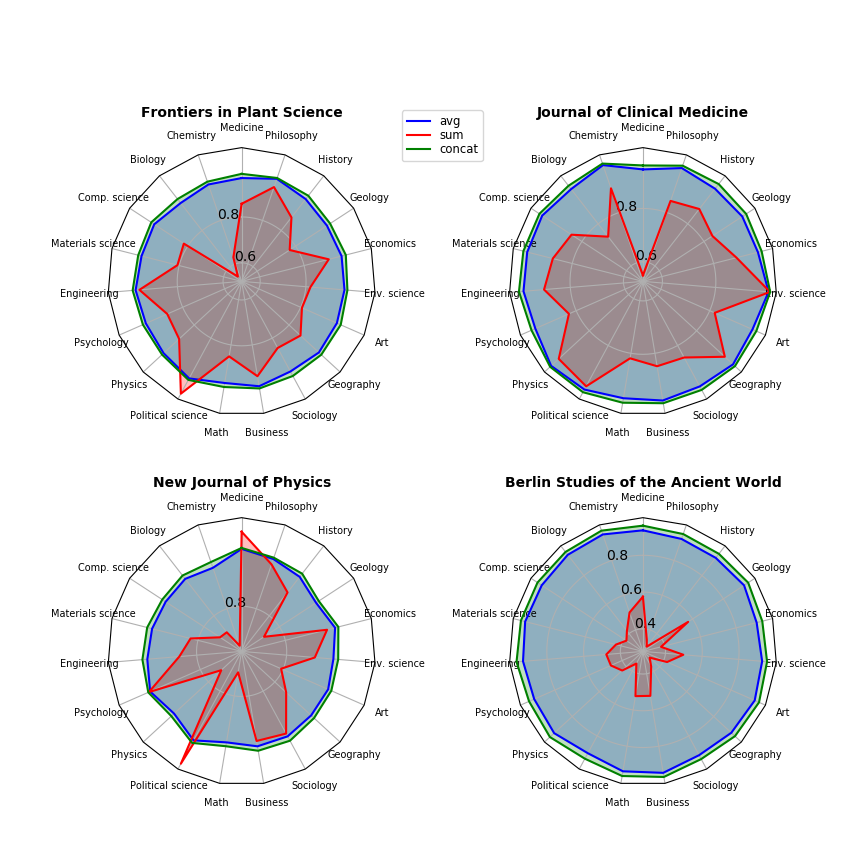
\includegraphics[width=\textwidth]{figures/unsupervised_approach/results/radar charts.png}
  \caption{Distances between venues and fields, for the three distance metrics.}
  \label{fig:combination_distance}
\end{figure}

In figure \ref{fig:combination_distance}, we show the results of the three methods for four venues, each belonging to a different field. The distances shown are the average distances of the documents that belong to each of the venues. In the upper left corner, the average distances of the documents that were published in \textit{Frontiers in Plant Science} are shown, which belongs to the field of \textit{Biology}. All three methods successfully identified the correct field on average.

The \textit{sum} method has the most expressive results. It assigns the documents \textit{Chemistry} in second place, and the distance between \textit{Biology} and \textit{Chemistry} exceeds $0.1$. On the other two methods, all three top options differ by around $0.01$. In fact, in the figures, one can see that the average distances of the concatenation and averaging methods are always around $0.95$. The difference between them occurs at a much lower scale. This shouldn't be a problem, as the distances can be rescaled afterwards.

All three methods also identified correctly the field of the venue \textit{Journal of Clinical Medicine}, shown in the upper right corner of figure \ref{fig:combination_distance}. Even for the averaging and concatenation methods, it is clear to see the smaller distance for the \textit{Medicine} field.

In the lower left corner, the average distances for the publications of \textit{New journal of Physics} are shown. None of the three methods places \textit{Physics} among their top three fields. The averaging and sum methods guess \textit{Chemistry} as the top field, whereas the concatenation method guesses \textit{Geology}. Physics is expected to be harder to guess because of its ubiquitous impact. It is closely related to other fields, mainly because it can be applied to any natural science.

The average distances between the fields and the documents published in \textit{Berlin Studies of the Ancient World}, which encompasses research in the fields of \textit{History} and \textit{Philosophy}, are shown in the lower left corner. The sum method was the only one to include both fields in their top three guesses, with \textit{Geography} between them. The other two methods guessed \textit{Political Science}, \textit{Economics} and \textit{Sociology}. Although similar, these were not the correct fields.
\subsection{Conclusion} \label{supervised_approach_conclusion}

We conclude this chapter by discussing the complexity of the implementation and some aspects of the model that may be improved to increase the performance of the model. The implementation of the models, as well as gathering the training data, is easy to develop. On the other hand, processing the training data training the models is computationally expensive.

We propose several improvements, mostly regarding the fact that the subject assignments are performed by an algorithm and not by a human. This means that its assignment noise could be modeled more easily, as the algorithms operates in a deterministic manner, whereas humans are not so consistent. Also, the assignment algorithm outputs confidence scores, which could also be used to improve the training procedure.

\subsubsection{Implementation}

The supervised approach was easy to implement. Gathering the training data didn't pose any difficulties because of the \acrshort{api} provided by OpenAlex. We vectorized the data in the same way we vectorized the documents of the repositories. Implementing the model also didn't pose any major challenges, as we used the architecture of related work \cite{gargiulo2019deep}. The further two papers we have implemented extended this initial model, both by modifying the loss function and one with an additional layer. Thus, the implementation time was much shorter than that of the unsupervised approach, which included numerous steps. On the other hand, this approach required training many models, which is computationally expensive. Processing the training data is also expensive.

\subsubsection{Room for improvement}

The hit rate of this approach can be easily improved by gathering more training data. Also, there are many techniques regarding the design and training of neural networks that may be experimented with, such as introducing batch or layer normalization \cite{ba2016layer}. Furthermore, there are two aspects from our use case that we have not considered:

\begin{enumerate}
    \item \textbf{Noise distribution}: model noise can be better modeled than human noise, because it is deterministic. Doing so would increase the performance of the model.
    \item \textbf{Confidence scores}: models output confidence scores for the subject assignments, which could be included in the training procedure, e.g. as a replacement of binary labels.
\end{enumerate}

Both aspects derive from the nature of our training dataset, which was created by an algorithm rather than by humans. Addressing these two points could lead to further improvements in the performance of the model. Label noise is a common topic in the literature, as it is present in all datasets labeled by humans because of their inconsistency (\cite{morris2010individual}, \cite{medelyan2008domain}). Deep networks must handle noise appropriately because, if not, they may overfit on the corrupted labels \cite{chen2019understanding}. There are three ways of handling noise \cite{karimi2020deep}: through the selection of the model and the loss function, by cleaning the data, or by developing a model that models label noise.

We have performed several data cleaning tasks, such as checking the language of the texts (see section \ref{repo_analysis_data}). Furthermore, the \acrlong{asl} models label noise better than \acrlong{bce}, as noise is not symmetric across positive and negative samples, given that positive ones are sparse \cite{zhao2021evaluating}. Still, modeling label noise may further increase the performance of the model, as our training data is estimated to have an assignment accuracy of 80 \% \cite{shen2018web}.

Confidence scores could be used instead of binary labels while training the models. This may help the model assess which subjects are closer thematically to the document. However, it may also introduce more noise.
\section{Supervised approach} \label{supervised_approach}

Our second approach to performing \acrshort{si} in the repositories is based on using external data to train a machine learning classifier, which will then be applied on the documents of the repositories. In machine learning, this field is called \acrfull{hmc}, as a variable number of labels may be assigned to any object, and the labels are organized in a hierarchy. The relevant literature was presented in chapter \ref{hmc}. The main challenge of the supervised approach is that the data used to train the classifier is noisy. The authors of \acrshort{mag}, whose data we are using, estimate that their subject indexing procedure has an accuracy of 80 \%.

This approach is fundamentally opposite to the unsupervised approach, which uses only data present in the repositories. The word embeddings and the vocabulary used in this approach are independent of the repositories, meaning that this classifier could be used without any modifications for any repository whose documents are topically similar to the ones used to train the classifier. This is an important difference between the approaches in terms of applicability, as the unsupervised approach is tailored specifically for our dataset, including numerous data cleaning steps and exception handling that are hard to generalize for their use in different scenarios.

Given that this approach should be widely applicable, we use pre-trained word embeddings. We present different in section \ref{supervised_approach_embeddings}. In the end, we use the fastText embeddings \cite{mikolov2017advances} because of their high accuracy and their similarity to the ones we trained ourselves in the unsupervised approach.

We then present and analyze the data we have gathered to train the models in section \ref{supervised_approach_data}. We have retrieved 200,000 documents from OpenAlex, each with a title, an abstract and a set of assigned subjects. As we want our training data to be well distributed across our subset of \acrshort{mag} subjects, we have retrieved up to 100 documents per subject.

In section \ref{supervised_approach_models}, we discuss our model architecture, which we have adopted from a similar use case \cite{gargiulo2019deep}. It includes two convolutional layers for feature extraction and two fully connected layers that compute assignment probabilities for each subject, given a document. We also implement two further extensions of the model. The first one only modifies the loss function to account for the imbalance between positive and negative samples in multi-label scenarios \cite{ben2020asymmetric}. The second one further extends the loss function by ensuring that the assignment probabilities don't violate the subject hierarchy \cite{giunchiglia2020coherent}. This enforcement is also performed by an additional layer we append to the first model.

We thus have three models. They all use the same neural network architecture, excepting the coherent model, which adds another layer on top. The main difference between the models is the loss function. Finally, in section \ref{supervised_approach_conclusion}, we talk about different aspects of this approach, such as its complexity and its computational cost. In summary, this approach is easy to implement but expensive to compute, as optimizing its parameters involves extensive experimenting. We also discuss potential improvements, such as modeling the label noise or introducing the confidence scores into the model.

\subsection{Embedding model} \label{implementation_skipgram}

To transform text into vectors, we first embed words into vector space. We could do so randomly, but this wouldn't take into account the semantic information of the words. To preserve this information, we use skip-gram \cite{mikolov2013distributed}, a word embedding model. This model was also used by \acrshort{mag} in their procedure. We already gave an overview of its design in section \ref{mag_skipgram}. In this section, we will look at how we trained the model and some examples of the resulting embeddings.

We train 100-dimensional word vectors, which we initialize with values sampled from the uniform distribution bounded by -1 and 1. The word vectors of \acrshort{mag} comprise 250 dimensions. We have decided to use fewer dimensions given that our vocabulary is much smaller: it includes around 50,000 entries, whereas \acrshort{mag}'s vocabulary has than 2 million.

We trained the model for 8 epochs. Surprisingly, it reached its best epoch loss already in the second iteration. The model optimized the embeddings quickly during the first epoch, starting with a batch loss of $30$ and ending with an average epoch loss of $4.9$. Figure \ref{fig:loss_avgs} shows the avg. loss of each epoch. Figure \ref{fig:loss_avgs_range} also shows the avg. loss, but with bars illustrating the range of the batch losses throughout the epoch.

\begin{figure}
  \begin{subfigure}[t]{0.5\textwidth}
    \centering
    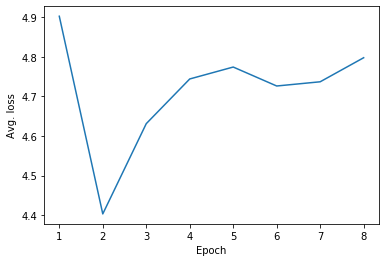
\includegraphics[width=\textwidth]{figures/unsupervised_approach/loss_avgs.png}
    \caption{Avg. training loss of each epoch.}
    \label{fig:loss_avgs}
  \end{subfigure}
  \hfill
  \begin{subfigure}[t]{0.5\textwidth}
    \centering
    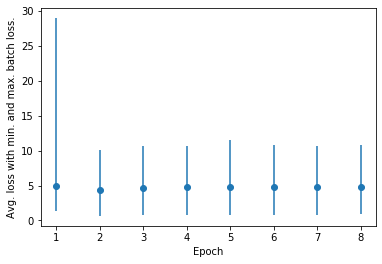
\includegraphics[width=\textwidth]{figures/unsupervised_approach/loss_avgs_range.png}
    \caption{The dots refer to the avg. epoch loss, while the extrema of the line refer to the min. and max. batch loss of that epoch.}
    \label{fig:loss_avgs_range}
  \end{subfigure}
  \caption{Plots of the training loss of the skip-gram model.}
\end{figure}


\subsubsection{Resulting embeddings}

We have computed the cosine distance between certain words to serve as an example. The cosine distance is also the metric we use to compare subjects and documents. The results can be found in table \ref{tab:embeddings_examples}. We have chosen three pairs of words, each of a different field. `polymer'' and ``monomer'' belong to the realm of chemistry; ``machine'' and ``learning'' usually refer to a family of algorithms; ``magnetic'' and ``resonance'' refer to a medical procedure. The chemistry pair is fed to the skip-gram model 96 times during training; the computer science pair, 1357 times and the medicine pair, 961 times.

Given that the cosine distance is symmetric, we only show one half of the table. Also, the distance of a vector to itself is zero. The table shows that the pairs of words of each field are closer to each other than to the other words. The distance between ``polymer'' and ``monomer'' is the largest of the three, which makes sense, as the model receives this pair of words hundreds of times less than the two others. The smallest distance between words that do not belong to the same field is between the words ``magnetic'' and ''polymer''. This distance is 34 \% larger than the distance between ``monomer'' and ``polymer''. Thus, the word vectors accurately differentiate between words that belong to the same field and those that don't.

As a further example of the semantic expressiveness of the embeddings, we can look at the word ``program'', although it belongs to the same field as the computer science pair, it is not as closely related to them. In fact, it appears 27 times as an input to the model with either of the words ``machine'' and ``learning''. However, this is more often as for the pairs of chemistry and medicine, with which it appears as input 26 and 3 times, respectively. The model was able to identify that ``program'' should be closer to the computer science pair, even if it appeared only one time less with the chemistry pair. Its cosine distance to ``machine'' and ``learning'' are 0.77 and 0.72, respectively. On the other hand, its cosine distance to the rest of the words is above 1.

\begin{table}[]
    \centering
    \begin{tabular}{c|c c c c c c}
       $dist(x,y)$ & monomer & polymer & machine & learning & magnetic  \\
       \hline
       resonance & 0.96 & 0.91 & 0.95 & 0.95 & \textbf{0.21} & \\
       magnetic & 0.88 & 0.82 & 0.98 & 0.98 & & \\
       learning & 1.08 & 1.19 & \textbf{0.41} & & & \\
       machine & 1.02 & 0.95 & & & & \\
       polymer & \textbf{0.54} & & & & & \\
    \end{tabular}
    \caption{Cosine distances between the vectors of certain words. The distances of words of the same field are highlighted in bold.}
    \label{tab:embeddings_examples}
\end{table}
\subsection{Training data} \label{supervised_approach_data}

In this section, we present the subset of \acrshort{mag} documents, which we use to train the supervised models. We first present how we have retrieved documents from the OpenAlex \acrshort{api} in section \ref{supervised_approach_data_retrieval}. We retrieve up to 100 documents for each subject in our subset, ensuring that each document has an abstract.

Then, in section \ref{supervised_approach_data_hierarchy}, we analyze the subject assignments of the documents. We focus on the consistency of the assignments regarding the hierarchy. If a document is assigned a subject, it should also have all its ancestors assigned. This is relevant for the model training, as hierarchy violations hinder the model's understanding of the subjects \cite{gargiulo2019deep}.

Finally, in section \ref{supervised_approach_data_result}, we discuss the resulting dataset. We have gathered over 200,000 documents. After correcting hierarchy violations, it comprises almost 2 million subject assignments. Only two subjects are not assigned to any documents, out of the 2,157 included in our subset.

\subsubsection{Document retrieval} \label{supervised_approach_data_retrieval}

To retrieve documents from OpenAlex, we iterate over the subjects in our subset of \acrshort{mag} subjects and look for journal articles that include each subject. We iterate over the resulting documents, and keep those that have an abstract and were not previously retrieved through another subject. The abstract of the documents is given as an inverted index, where each word is mapped to its positions in the abstract. This was done for copyright reasons.

We have retrieved up to 100 documents per subject, and stored them in multiple files, with max. 3,000 documents per file. For each document, we first build the abstract and append it to the title. We then process the resulting text, and store it in a file together with its assigned subjects. The processing involves tokenizing and lemmatizing the data, just as it was done for the texts of the repositories (see section \ref{implementation_vocab}). We also discard stopwords and tokens that have less than three letters, which removes numbers, symbols and quantities (e.g. 100mg).

\subsubsection{Hierarchy violations} \label{supervised_approach_data_hierarchy}

Here we look at the subject assignments of the documents presented above, looking for inconsistencies regarding the hierarchy of subjects, before presenting the final training dataset. The assignments of a document are inconsistent if the ancestors of an assigned subject are not assigned as well. We consider this a violation of the hierarchy.

There are 1,952 documents that are not assigned a \acrshort{mag} field, which are therefore inconsistent, as they are assigned subjects of further levels but not from the first. Interestingly, 122 of these documents have the subject \textit{Mechanics} assigned to them. 427 of these documents without assigned fields only have one assigned subject. On average, these subjects are assigned 1.2 subjects, with 1,582 distinct subject assignments. We have corrected these violations using the lists of ancestors of the subjects. The resulting dataset is presented in the next section.

\subsubsection{Resulting dataset} \label{supervised_approach_data_result}

\begin{figure}
    \centering
    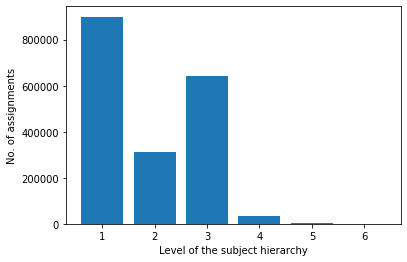
\includegraphics[width=.7\textwidth]{figures/supervised_approach/training_data_levels.png}
    \caption{Number of subject assignments per hierarchy level.}
    \label{fig:training_data_levels}
\end{figure}

Following the retrieval procedure outlined above, we could gather 214,538 documents, comprising 100 documents for all subjects except for 17. When looking at all assignments, there are two subjects of our subset for which we could not retrieve any documents: \textit{Algorithm design} and \textit{Premise}. There are two further subjects for which we could not retrieve any documents (\textit{Shoot} and \textit{Intensive care unit}), but they are present in more than 300 documents each, when looking at the whole dataset. This occurs because the only documents that include these subjects were already retrieved by looking at the documents assigned with other subjects.

In total, there are 1,890,080 subject assignments. 821,273 of these assignments were added to fix hierarchy violations. The field that has benefited the most from fixing the hierarchy violations is \textit{Engineering}, which went from being the field with the least assignments (2,565), to having over 60,000 assignments. All fields have more than 20,000 assignments after the corrections, whereas before there were several with less than 5,000 assignments.

As shown in \ref{fig:training_data_levels}, most of them belong to the first hierarchy level. Here, only the field assignments are considered. \textit{Biology} is the most assigned field, with over 80,000 assignments. \textit{Art} has the least assignments, with just over 20,000. Among the other levels of the hierarchy, the most popular subjects are \textit{Law}, with 49,842 assignments and \textit{Ecology}, with 37,136 assignments. Both had less than 10,000 assignments before fixing the hierarchy violations.

Although we have avoided duplicates by keeping the OpenAlex IDs of the retrieved documents, there are 4,849 documents with the same data. 122 of them are documents for which no tokens remained after the filtering procedure, and 31 of them have uninformative texts like review appeals. The remaining documents are actual duplicates, with the same data appearing in at most three documents. There are 2,346 distinct documents among them, with an average of one duplicate per document. Thus, the final number of distinct documents is 212,035.

\begin{figure}
    \centering
    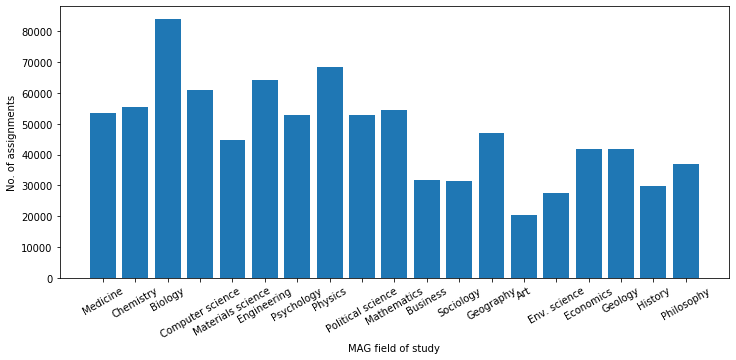
\includegraphics[width=\textwidth]{figures/supervised_approach/training_data_fields.png}
    \caption{Distribution of the documents across the MAG fields of study.}
    \label{fig:training_data_fields}
\end{figure}
\subsection{Our classifiers} \label{supervised_approach_models}

We implement the convolutional neural network detailed in \cite{gargiulo2019deep}, as their use case closely resembles ours (see section \ref{hmc_gargiulo}). They also work with scientific texts and assign to them subjects organized in a hierarchy. The paper provides a complete architecture, from processing the text, to extracting features and feeding them to a classifier. Their architecture is grounded on previous work, which makes their design decisions more sound. Our use cases differ mainly in three points:

\begin{enumerate}
    \item \textbf{Training data}: they have over eleven million documents, two orders of magnitude more than us.
    \item \textbf{Label noise}: their subject indexing procedure was performed by humans, whereas ours was performed by an unsupervised algorithm, which is not as accurate.
    \item \textbf{Subject hierarchy}: theirs comprises more than 20,000 subjects, one order of magnitude more than us.
\end{enumerate}

We consider these differences when adapting the architecture for our case. We discuss the design choices of the original architecture and the changes we have made in section \ref{supervised_approach_design}. These include reducing the size of the model, given our smaller number of labels and our shorter inputs, increasing the dropout probability, which was very low in the original implementation, and using a learning rate schedule instead of keeping it constant.

In section \ref{supervised_approach_add_asymmetry}, we replace the loss function of our model with one specifically designed for \acrfull{mlc} \cite{ben2020asymmetric} that decouples positive from negative labels, which allows the model to focus on the rare positive samples instead of on the numerous negative ones. See section \ref{hmc_asl} for more details. This loss function was used in \cite{zhao2021evaluating} to evaluate \acrshort{mlc} with noisy labels, concluding that it increased the regularization of the model, thus avoiding overfitting the noisy data. Therefore, this loss function may help us address label noise, the second difference between the original use case and ours.

The second extension we implement is the addition of the \acrlong{mcm} and using the \acrfull{mcl} \cite{giunchiglia2020coherent} as our model's loss function. To the best of our knowledge, it is the current \acrshort{sota} for \acrshort{hmc}. The paper was already presented in section \ref{hmc_forward}. Given that both the \acrshort{asl} and the \acrshort{mcl} extend the \acrshort{bce}, we combine them, yielding the \acrlong{aml}, which we use for this model.

We thus have three models. They only differ on the loss function, and the additional layer of the coherent model. All other model parameters, as well as the training settings, are the same. For brevity, we refer to each of the three models by their loss function: the \acrshort{bce} model, the \acrshort{asl} model and the \acrshort{aml} model. We present their architecture and parameters in the following sections.

\subsubsection{Design of the classifying pipeline} \label{supervised_approach_design}

\begin{figure}
    \centering
    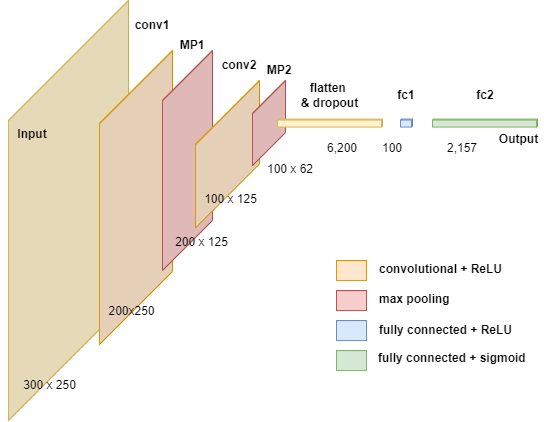
\includegraphics[width=.85\textwidth]{figures/supervised_approach/model_diagram.png}
    \caption{Diagram of the model. The shown sizes are the outputs of each layer.}
    \label{fig:model_diagram}
\end{figure}

Our model comprises two phases: one where feature extraction is performed, and a second one where the probabilities of each subject being assigned to the input document are computed. We first define the input to the model, which is not the same as for the original implementation (i.e. the one from \cite{gargiulo2019deep}), given our different use cases. We use only one representation type instead of four, and we keep the first 250 words of each text, instead of the first 400. Then, we explain the architecture of the model. We adapt the original implementation to our use case, and also optimize several aspects through experimentation. Please note that a description of how convolutions are applied to text was given in section \ref{hmc_cnn}.

\paragraph{Input} \mbox{}

The input to the model is a collection of word vectors. In the original implementation, they pick the first 400 words of each text and discard the rest. If a text has less than 400 words, they pad it with zero vectors. As shown in figure \ref{fig:sm_doc_length}, most of our documents have less than 250 tokens. We therefore pick 250 as our threshold, and also pad when necessary. Some representations are very short because the documents don't have abstracts, or because they are written in other languages and tagged as they were in English (see section \ref{repo_analysis_data}).

We only consider the tokens for which we have a pre-trained vector. The fastText word vectors are 300-dimensional, meaning they comprise 300 floating numbers each. Thus, the input is formed by 250 word vectors, each with 300 dimensions. As shown in figure \ref{fig:model_diagram}, the input forms a matrix, where each word vector is a column.

\begin{figure}
    \centering
    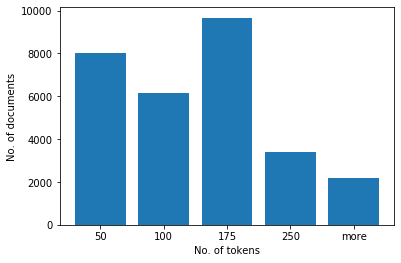
\includegraphics[width=.6\textwidth]{figures/supervised_approach/sm_doc_length.png}
    \caption{No. of tokens per document, in five groups.}
    \label{fig:sm_doc_length}
\end{figure}

\paragraph{Model architecture} \mbox{}

The feature extraction phase comprises two convolutional layers, each followed by ReLU activation and a max-pooling layer. Both pooling layers have a kernel size of 2, and both convolutional layers have stride 1. The stride defines the steps taken across the input between convolutions. Furthermore, both convolutional layers use padding to keep the number of dimensions unaltered

The first convolutional layer has 200 filters and kernel size 5. The number of filters is the number of features extracted from the input. Thus, the resulting matrix has 200 rows and the same number of columns, as shown in figure \ref{fig:model_diagram} in the \textit{conv1} layer. The kernel size defines how large a context window should be considered for each word vector. The second convolutional layer has 100 filters and kernel size 3. The resulting matrix, which comprises 100 rows and 62 columns, is flattened into a one-dimensional vector. Then, its constituent elements are zeroed with a certain dropout probability, a regularization technique used to avoid overfitting. The probability of this layer is discussed in the following section.

The assignment probabilities for each document are computed by a classifier consisting of two fully connected layers. The size of the output is equivalent to the number of subjects, as we want to output an assignment probability for each of them. The output layer also has sigmoid activation instead of ReLU, so each probability is between zero and one. The size of the first layer, called the hidden layer, comprises 1,024 neurons in the original paper, as their number of subjects exceeds 20,000. Given that our set of subjects is one order of magnitude smaller, we have reduced the size of the hidden layer. We experiment with 100 and 200 neurons in appendix \ref{supervised_approach_optim}. As both values perform similarly, we keep the lower one for further regularization and less computational cost.

\subsubsection{Training parameters} \label{supervised_approach_params}

The model parameters are optimized using \acrfull{sgd}, where the gradient is estimated by considering only a subset of the data. It is a trade-off between computational cost and fast convergence rate, parameterized by the batch size. A larger batch size accelerates convergence (regarding the number of steps), but also increases the computational cost. The original implementation uses a batch size of 10 and improve the convergence rate with a Nesterov momentum of $0.5$. Momentum introduces inertia into the gradient space, meaning that the direction of the steps are influenced by previous steps. They use \acrfull{bce} as a loss function. As discussed in section \ref{hmc_asl}, this is the common loss function for multi-label settings.

We experimented with two different sizes for the hidden layer: 100 and 200. The results showed that both sizes performed similarly. We decided to keep the lower size, which reduces the computational cost and increases regularization. We also experimented with two values for the dropout probability which were common in the literature: 30 \% and 70 \%, concluding that the higher value offers better results. The original implementation used a dropout probability of 10 \%, which is very low when compared with the literature. Both experiments can be found in appendix \ref{supervised_approach_optim}.

Interestingly, the original implementation doesn't use a learning rate (LR) scheduler, which is common practice in deep learning. Instead, they keep the LR constant at $0.1$. This is not optimal, both in terms of efficiency and accuracy. Gradient steps should be larger when further away from the optimum, to increase convergence rate, and decrease over time to not overshoot the optimum. Our experiments, presented in appendix \ref{supervised_approach_optim}, show that the 1-cycle policy fits our use case better than a decaying LR schedule. Cyclical LR schedules \cite{smith2017cyclical} follow the observation that increasing the LR may lead the model to perform better in the long term. The 1-cycle policy increases the LR until it reaches a given maximum, and then decreases it monotonically afterwards.

\subsubsection{Adding asymmetry} \label{supervised_approach_add_asymmetry}

Our first extension of the model described above, which we term \acrshort{bce} model because of its loss function, is to replace its loss function with the \acrfull{asl}, resulting in the \acrshort{asl} model. The \acrshort{asl}, which was already presented in section \ref{hmc_asl}, extends the \acrfull{bce} loss to address the imbalance between positive and negative samples in multi-label settings. It receives two parameters, $\gamma_-$ and $\gamma_+$. They modulate the importance of negative and positive samples, respectively. The larger their values, the lower the impact of their corresponding samples on the result of \acrshort{asl}.

We have experimented with these parameters in appendix \ref{supervised_approach_asymmetric}, concluding that the optimal values for our use case are $\gamma_+=1$ and $\gamma_-=2$. Recall that the \acrshort{asl} model is exactly the same as the \acrshort{bce} model, except for the loss function.

\subsubsection{Adding coherence} \label{supervised_approach_add_coherence}

The second extension of the \acrshort{bce} model is the addition of a new layer, called the \acrfull{mcm}, and the use of the \acrfull{aml}. The \acrshort{mcm}, which was presented in section \ref{hmc_forward}, enforces the subject hierarchy upon the output of the model, so subjects have an assignment probability at least as high as the assignment probabilities of their descendants. In practice, the \acrshort{mcm} is implemented as a matrix, where each row has ones for the subject it represents and its descendants, and zeros otherwise. Each row of this matrix is multiplied element-wise with the output of the model. Then, the maximum of each row is assigned to the corresponding subject.

The loss function used by the original coherent model \cite{giunchiglia2020coherent}, called the \acrfull{mcl}, modifies \acrshort{bce} loss to also ensure that the assignment probabilities respect the subject hierarchy. Given that the \acrshort{asl} also extends  \acrshort{bce}, we can combine them. Below is a comparison of all three loss functions, and their resulting combination, which we term \acrfull{aml}. In these formulas, $D(x)$ is the set of subjects that are descendants of subject $x$. All the individual losses are then averaged to arrive at the final loss for a document, which has as many of these input-output pairs as there are subjects.

\begin{align*}
    & BCE(x, y) = -y \cdot \log (x) - (1-y) \cdot \log (1-x) \\ \\
    & ASL_{\gamma_-, \gamma_+}(x, y) = -y \cdot \log (p) \cdot (1-p)^{\gamma_+} - (1-y) \cdot \log (1-p) \cdot p^{\gamma_-} \\ \\
    & MCL(x, y) = -y \cdot \log (\max(x, \{x_d \cdot y_d, \forall d \in D(x)\}) - (1 - y) \cdot \log (1 - MCM_x) \\ \\
    & AML_{\gamma_-, \gamma_+}(x, y) = -y \cdot \log (\max(x, \{x_d \cdot y_d, \forall d \in D(x)\}) \cdot (1-p)^{\gamma_+} \\
    & \qquad \qquad \qquad \qquad - (1 - y) \cdot \log (1 - MCM_x) \cdot p^{\gamma_-} \\
\end{align*}

We have performed an experiment to compare the \acrshort{mcl} with the \acrshort{aml}, outlined in appendix \ref{supervised_approach_coherence}, concluding that \acrshort{aml} performs better in our dataset. We thus use the \acrshort{aml} in our third supervised model.
\subsection{Conclusion} \label{supervised_approach_conclusion}

We conclude this chapter by discussing the complexity of the implementation and some aspects of the model that may be improved to increase the performance of the model. The implementation of the models, as well as gathering the training data, is easy to develop. On the other hand, processing the training data training the models is computationally expensive.

We propose several improvements, mostly regarding the fact that the subject assignments are performed by an algorithm and not by a human. This means that its assignment noise could be modeled more easily, as the algorithms operates in a deterministic manner, whereas humans are not so consistent. Also, the assignment algorithm outputs confidence scores, which could also be used to improve the training procedure.

\subsubsection{Implementation}

The supervised approach was easy to implement. Gathering the training data didn't pose any difficulties because of the \acrshort{api} provided by OpenAlex. We vectorized the data in the same way we vectorized the documents of the repositories. Implementing the model also didn't pose any major challenges, as we used the architecture of related work \cite{gargiulo2019deep}. The further two papers we have implemented extended this initial model, both by modifying the loss function and one with an additional layer. Thus, the implementation time was much shorter than that of the unsupervised approach, which included numerous steps. On the other hand, this approach required training many models, which is computationally expensive. Processing the training data is also expensive.

\subsubsection{Room for improvement}

The hit rate of this approach can be easily improved by gathering more training data. Also, there are many techniques regarding the design and training of neural networks that may be experimented with, such as introducing batch or layer normalization \cite{ba2016layer}. Furthermore, there are two aspects from our use case that we have not considered:

\begin{enumerate}
    \item \textbf{Noise distribution}: model noise can be better modeled than human noise, because it is deterministic. Doing so would increase the performance of the model.
    \item \textbf{Confidence scores}: models output confidence scores for the subject assignments, which could be included in the training procedure, e.g. as a replacement of binary labels.
\end{enumerate}

Both aspects derive from the nature of our training dataset, which was created by an algorithm rather than by humans. Addressing these two points could lead to further improvements in the performance of the model. Label noise is a common topic in the literature, as it is present in all datasets labeled by humans because of their inconsistency (\cite{morris2010individual}, \cite{medelyan2008domain}). Deep networks must handle noise appropriately because, if not, they may overfit on the corrupted labels \cite{chen2019understanding}. There are three ways of handling noise \cite{karimi2020deep}: through the selection of the model and the loss function, by cleaning the data, or by developing a model that models label noise.

We have performed several data cleaning tasks, such as checking the language of the texts (see section \ref{repo_analysis_data}). Furthermore, the \acrlong{asl} models label noise better than \acrlong{bce}, as noise is not symmetric across positive and negative samples, given that positive ones are sparse \cite{zhao2021evaluating}. Still, modeling label noise may further increase the performance of the model, as our training data is estimated to have an assignment accuracy of 80 \% \cite{shen2018web}.

Confidence scores could be used instead of binary labels while training the models. This may help the model assess which subjects are closer thematically to the document. However, it may also introduce more noise.
\section{Evaluation} \label{eval}

In this chapter, we present our evaluation procedure, which we use to assess the performance of the approaches. We have created three evaluation sets with the metadata from the repositories. Two of them consider only fields, whereas the third one considers all subjects. We evaluate the approaches on these sets with two different metrics, one that measures the hit rate of the assignments and one that uses the hierarchy to evaluate if the guesses are close to the correct subject. 

We discard performing a survey because every sample would require cross-checking, as human judges are inconsistent \cite{csomai2007investigations}. Furthermore, given how technical our documents are, assessing the appropriateness of a subject assignment might prove difficult for someone who is not well-read in the topics of the document. Another disadvantage is that numerous assignments have to be evaluated for the survey to gain statistical significance. Thus, we would need to gather experts in various fields (multiple per field) and have them assess many assignments. We therefore leave the survey for future work.

As we discussed when analyzing the repositories (section \ref{repo_analysis_subjects}), most of the popular subjects in the repositories are \acrfull{ddc} subjects. These are usually broader in their meaning, but are still useful descriptors of the topics handled by a document. We present how we have incorporated them into our evaluation procedure in section \ref{eval_ddc}. Essentially, given that we have to manually assign them to \acrshort{mag} subjects, we have mapped them to the fields. They will therefore be useful to evaluate if the indexing methods have grasped the broad meaning of the documents.

Venues, advisors and referees also describe the content of the documents they are assigned to. We therefore create another evaluation set with them. As for the \acrshort{ddc} evaluation set, in section \ref{eval_venues} we map popular venues, advisors and referees manually to the fields of study, and then retrieve their associated documents.

We create our final evaluation set by automatically mapping subjects present in the repositories to the ones in our subset of \acrshort{mag} subjects. This evaluation set is the only one that considers subjects that are not fields, and is thus the one that determines is the approach is able to correctly model the 2,157 labels we consider in this thesis.

We measure the performance of the models on these evaluation sets with two different metrics. The first outputs one if the correct subject is included in the top $k$ subjects output by a model, and otherwise zero. The second one, given a subject and a candidate output by a model, outputs a value between zero and one that describes how close the candidate is to the subject in the hierarchy. We present both metrics in section \ref{eval_metrics}, as well as other metrics we have found in the literature.

After presenting the evaluation sets and metrics, we use them to compare the candidates of each approach and then compare the resulting models to one another. Interestingly, our evaluation procedure indicates that our own word embeddings yield better results in the unsupervised approach than pre-trained embeddings. Regarding the supervised approach, we find out that extending the model with asymmetry or coherence does not improve the performance of the model, which may be because some parameters were optimized for the initial model, without considering the two extensions. Still, the supervised approach yields the best results in all evaluation sets and for both metrics.

We end this chapter by analyzing the impact of representation length on the hit rate of the supervised model. We find out that the hit rate of the model for documents that are represented by less than 50 tokens is over 20 \% worse than for larger representations. This indicates that our results could be improved by adding missing abstracts, and fixing those that are in other languages.

\subsection{Evaluation sets} \label{eval_datasets}

Subject assignments can be evaluated with the metadata of the documents. \cite{toepfer2020fusion} mentions this possibility, stating that they plan on developing an automatic quality estimation metric that is based on meta information of the documents. For example, documents that are published in the same journal can be expected to be semantically similar. The publisher clearly delimits the field to which the publication belongs to. Our approach, although it also uses the metadata to evaluate the methods, is more straight forward. We extract subjects and venues (including referees and advisors of theses) from the repositories to construct three evaluation sets.

The first evaluation set comprises the handwritten subjects of the repositories, i.e. those that the users input manually when uploading a new document. We have mapped our complete set of subjects to the handwritten subjects of the repositories with a string matching procedure. Doing so, we could create an evaluation set with over 9,000 assignments. This evaluation set is the only one that considers further subjects, other than fields.

\acrshort{ddc} subjects can also be used in this regard. They appear consistently throughout all three repositories, as shown in section \ref{subjects_ddc}, and don't suffer from potential duplicates that arise from the free-text input, as handwritten subjects do. We have manually mapped \acrshort{ddc} numbers to \acrshort{mag} fields of study, to construct our second evaluation set.

Using unsupervised methods to evaluate the set of subjects of theses may prove more challenging, as they are not published anywhere and their authors usually just have that one document in the repositories. Advisors and referees may be of use in this regard. Two theses advised by the same professor should be more similar than two theses advised by different professors. This is the same logic we followed in the \acrfull{um}. We create our third evaluation set by manually mapping venues, advisors and referees to \acrshort{mag} fields of study.

\subsubsection{Handwritten subjects} \label{eval_subjects}

We have mapped our subset of \acrshort{mag} subjects to those of the repositories, which were input manually by the users that uploaded the documents, hence the term ``handwritten subjects''. To increase the number of matches, we have done so in a case-insensitive manner, i.e. we have first lower-cased all subjects. This simple matching procedure yielded 1,272 subjects, meaning that 59 \% of our \acrshort{mag} subset is present in the repositories. The total number of assignments of subjects to documents is 9,052.

The most popular subjects are \textit{Climate change}, which is assigned to 154 documents, \textit{Sustainability}, with 124 assignments, \textit{Mass spectrometry}, with 87 assignments and \textit{Molecular dynamics}, with 76 assignments. Figure \ref{fig:docs_per_subject} shows how often each subject occurs in the repositories. 301 subjects are assigned to only one document, whereas 307 subjects are assigned to at least nine documents. On average, the subjects are assigned to seven documents of the repositories.

\begin{figure}
  \begin{subfigure}[t]{0.45\textwidth}
    \centering
    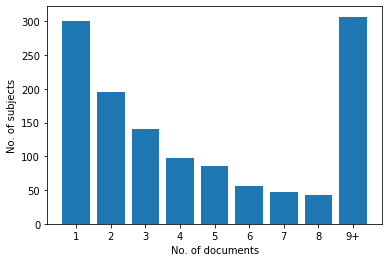
\includegraphics[width=\textwidth]{figures/evaluation/docs_per_subject.png}
    \caption{Handwritten subjects.}
    \label{fig:docs_per_subject}
  \end{subfigure}
  \hfill
  \begin{subfigure}[t]{0.45\textwidth}
    \centering
    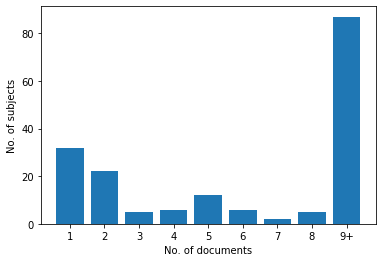
\includegraphics[width=\textwidth]{figures/evaluation/docs_per_ddc.png}
    \caption{DDC subjects.}
    \label{fig:docs_per_ddc}
  \end{subfigure}
  \caption{Distribution of the number of documents each subject (handwritten or DDC) is assigned to.}
\end{figure}

Another positive aspect of these subject matches is how well distributed they are across the fields. As can be seen in figure \ref{fig:eval_hw_fields}, all fields have assignments. \textit{Environmental science} is the least populated field, with 41 assignments. On the other hand, \textit{Medicine}, \textit{Biology} and \textit{Physics} have more than 200 assignments each.

\begin{figure}
  \begin{subfigure}[t]{\textwidth}
    \centering
    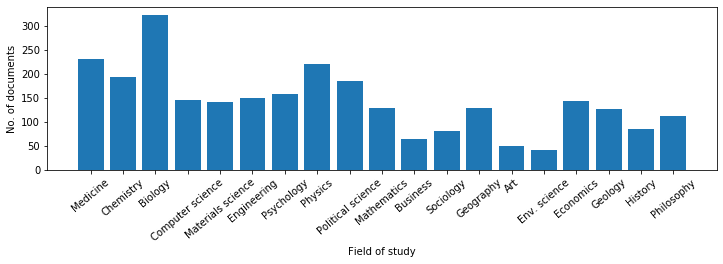
\includegraphics[width=\textwidth]{figures/evaluation/eval_hw_fields.png}
    \caption{Handwritten subjects}
    \label{fig:eval_hw_fields}
  \end{subfigure}
  \hfill
  \begin{subfigure}[t]{\textwidth}
    \centering
    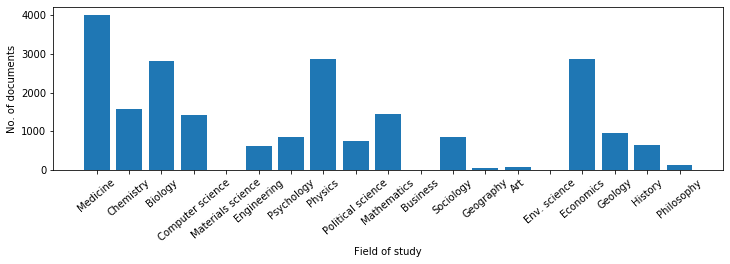
\includegraphics[width=\textwidth]{figures/evaluation/eval_ddc_fields.png}
    \caption{DDC subjects}
    \label{fig:eval_ddc_fields}
  \end{subfigure}
  \begin{subfigure}[t]{\textwidth}
    \centering
    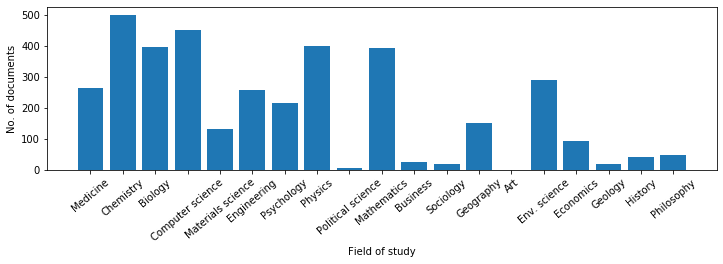
\includegraphics[width=\textwidth]{figures/evaluation/eval_venue_fields.png}
    \caption{Venues}
    \label{fig:eval_venue_fields}
  \end{subfigure}
  \caption{Number of assignments per field of study for handwritten subjects, DDC subjects and venues.}
\end{figure}

This evaluation set comprises 7,145 distinct documents. 78 \% of them only have one of the \acrshort{mag} subjects assigned to them, as shown in figure \ref{fig:eval_hw_fields}. On average, documents are assigned 1.27 subjects. Only one document has more than six assignments. It belongs to edoc and its subjects include \textit{Sustainability}, \textit{Climate change} and \textit{Poverty}, among others. Then there are two documents of refubium with six assignments, one about public law and the other about magnesium, potassium and other chemical elements.

The documents are also evenly distributed across repositories. Refubium has the largest amount of documents in this evaluation set, with 3,208. This makes sense, given that it contains 47 \% of all the documents in our dataset. Depositonce has 2,192 documents and edoc, 1,745. As percentages of their total number of documents, all repositories have more than 20 \% of their documents in this evaluation set. Depositonce leads the way with 29 \%, followed by edoc, with 23 \%, and refubium, with 22 \%.

\begin{figure}
  \begin{subfigure}[t]{0.45\textwidth}
    \centering
    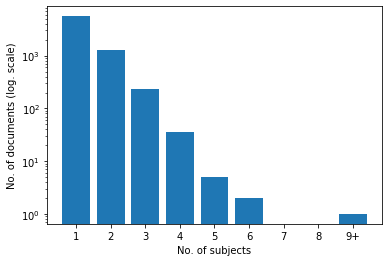
\includegraphics[width=\textwidth]{figures/evaluation/subjects_per_doc.png}
    \caption{Handwritten subjects.}
    \label{fig:subjects_per_doc}
  \end{subfigure}
  \hfill
  \begin{subfigure}[t]{0.45\textwidth}
    \centering
    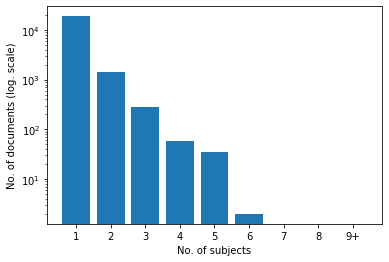
\includegraphics[width=\textwidth]{figures/evaluation/ddc_per_doc.png}
    \caption{DDC subjects.}
    \label{fig:ddc_per_doc}
  \end{subfigure}
  \caption{Number of subjects (handwritten or DDC) assigned to each document.}
\end{figure}

\subsubsection{DDC subjects} \label{eval_ddc}

Mapping \acrshort{ddc} subjects to \acrshort{mag} subjects was more complicated than with the handwritten subjects of the repositories, as they are numbers and cannot be mapped through a basic string matching procedure. In section \ref{eval_ddc_map}, we show how we have manually mapped \acrshort{ddc} number to the \acrshort{mag} fields of study. We could find \acrshort{ddc} numbers for all fields except for \textit{Materials science}, \textit{Business} and \textit{Environmental science}.

We present the resulting evaluation set in section \ref{eval_ddc_results}. It comprises over 22,000 assignments, including 70 \% of all documents, making this evaluation set the largest of the three. Depositonce is the repository that is worse represented by this set, with a coverage of 31 \%.

\paragraph{Mapping procedure} \mbox{} \label{eval_ddc_map}

We have manually mapped \acrshort{ddc} subclasses to the \acrshort{mag} fields of study. This is straight forward, as most of the fields of study have equivalent \acrshort{ddc} subclasses. For example, \textit{Biology} is a field in \acrshort{mag} and also a \acrshort{ddc} subclass, with the number $570$. The same is true for almost all fields, except for \textit{Materials Science}, \textit{Business} and \textit{Environmental Science}. \textit{History} and \textit{Philosophy}, on the other hand, have multiple \acrshort{ddc} subclasses, as their broad subjects are divided into more concrete fields. For example, \textit{History} has one subclass per continent, as well as others. The whole mapping of \acrshort{ddc} subclasses to \acrshort{mag} fields is depicted in table \ref{tab:ddc_fields}.

\begin{table}[]
    \centering
    \begin{tabular}{|c|c|}
        \hline
        \textbf{MAG field} & \textbf{DDC subclasses} \\ \hline\hline
        Medicine & 610 \\ \hline
        Chemistry & 540 \\ \hline
        Biology & 570 \\ \hline
        Computer Science & 000 \\ \hline
        Materials Science &  \\ \hline
        Engineering & 620 \\ \hline
        Psychology & 150 \\ \hline
        Physics & 530 \\ \hline
        Political Science & 320 \\ \hline
        Mathematics & 510 \\ \hline
        Business &  \\ \hline
        Sociology & 300 \\ \hline
        Geography & 910 \\ \hline
        Art & 700 \\ \hline
        Environmental Science &  \\ \hline
        Economics & 330 \\ \hline
        Geology & 550 \\ \hline
        History & 900, 910, 940-990 \\ \hline
        Philosophy & 100, 120, 140-190 \\ \hline
    \end{tabular}
    \caption{Manual mapping of DDC subclasses to MAG fields of study.}
    \label{tab:ddc_fields}
\end{table}

All \acrshort{ddc} subclasses and more specific subjects under each of the subclasses shown in table \ref{tab:ddc_fields} are also included in our evaluation set. For instance, the \acrshort{ddc} subject \textit{Philosophy of Germany and Austria}, number $193$, is a descendant of the \acrshort{ddc} subclass \textit{Modern western philosophy}, which has the number $190$. We therefore include all \acrshort{ddc} numbers that start with $19$ (or any other number of table \ref{tab:ddc_fields}) in our evaluation set.

\paragraph{Evaluation set} \mbox{} \label{eval_ddc_results}

Applying the mapping procedure explained above yields an evaluation set that comprises 22,915 assignments. As can be seen in figure \ref{fig:eval_ddc_fields}, \textit{Medicine} is by far the most popular field, with 3,611 assignments. \textit{Physics}, \textit{Biology} and \textit{Economics} also have more than 2,000 assignments. In total, this set comprises 20,636 documents, which amount to 70 \% of the 29,399 documents in our dataset. 18,865 of them have only one \acrshort{ddc} subject assigned to them, whereas two documents have six \acrshort{ddc} subjects. The number of \acrshort{ddc} subjects per document is depicted in figure \ref{fig:eval_ddc_fields}. On average, documents are assigned 1.1 \acrshort{ddc} subjects.

Regarding the repositories, depositonce is the repository with the least assignments. 2,333 of its documents have been assigned \acrshort{ddc} subjects, which accounts for 31 \% of its documents. Edoc and refubium, on the other hand, have \acrshort{ddc} subjects assigned to 77 \% and 86 \% of their documents, respectively. Figure \ref{fig:docs_per_ddc} shows how frequently \acrshort{ddc} subjects are assigned to documents. 49 \% of the \acrshort{ddc} subjects are assigned to at least nine documents. On the other hand, 32 \% are assigned to only one document. On average, \acrshort{ddc} subjects are assigned to 129 documents.

In total, there are 177 distinct \acrshort{ddc} subjects. 28 of them are classes or subclasses, i.e. their numbers end in $0$, and the rest are more specific. The classes and subclasses, having larger scopes, are assigned to 623 documents on average, whereas the rest of the \acrshort{ddc} subjects are assigned to 37 documents, on average. \textit{History} has by far the most distinct \acrshort{ddc} subjects, with 41, followed by \textit{Philosophy}, with 18. \textit{Art} is the field with the least \acrshort{ddc} subjects, with six (ignoring the three fields that could not be mapped to any \acrshort{ddc} subclasses).

\subsubsection{Venues} \label{eval_venues}

Venues are also good descriptors of the topics handled by a publication. They are similar to \acrshort{ddc} subjects in their scope; they can't be used to evaluate the most specific subjects, but can be useful to assess if the indexing procedures are guessing the right \acrshort{mag} field of study of each document.

Mapping venues to fields must also be done manually. We perform a similar procedure as was done for the \acrshort{ddc} subjects in the previous section. We therefore also divide this section in two parts: how venues were mapped to subjects, and then the resulting evaluation set.

\paragraph{Mapping procedure} \mbox{}

As mentioned in section \ref{repo_analysis_venues}, there are 4,418 distinct venues, 2,867 of which (65 \%) are only assigned to one publication. We therefore filter out the most popular ones, i.e. those that appear in at least ten documents. Recall that we also consider advisors and referees, so that theses can be grouped as well. There are 70 venues, 13 advisors and 70 referees with more than ten documents. From now on, we also refer to advisors and referees when we mention venues, as that is their role in this section.

The venues with more than 10 documents cover only the most popular fields. We therefore had to look online for professors of disciplines that were not present in this list of venues, such as \textit{Geology}, \textit{Sociology}, or \textit{Business}. In the end, we have manually assigned 132 venues to the \acrshort{mag} fields. \textit{Art} is the only field for which we could not find any venue in the repositories. The mapping of venues to fields can be found in Appendix \ref{appendix_venue_map}. There you can also find how many documents belong to each venue.

Although it is not relevant for this evaluation set, it is worth noting the presence of duplicates in the lists of referees and advisors. While mapping professors to \acrshort{mag} fields, we sometimes found the same professor under different names. For example, Prof. Dr. Charlotte M. Krawzcyk appears in the repositories under six different names, and Prof. Dr. Michael C. Burda, under five different names. This issue was already mentioned in section \ref{repo_analysis_contributors}.

\paragraph{Evaluation set} \mbox{}

Once we have assigned the venues to the \acrshort{mag} fields, we can use this mapping to assign documents to fields, just as we did to create the \acrshort{ddc} evaluation set. Figure \ref{fig:eval_venue_fields} shows the distribution of documents in this evaluation set per field. As happened with the evaluation sets derived from the subjects, the natural sciences are better represented than the social sciences. \textit{Chemistry} has the most documents, with 499, followed by \textit{Computer Science} and \textit{Physics}, with 449 and 399 documents, respectively. \textit{Art}, \textit{Political science} and \textit{Geology} are the worst represented fields, with 0, 8 and 21 documents, respectively.

An important difference between this evaluation set and the other two is how well represented \textit{Environmental science} is. In the evaluation set derived from the handwritten subjects, this field had the least documents, with 41 documents, and in the \acrshort{ddc} evaluation set it had none. Here it has 291 documents.

\begin{figure}
    \centering
    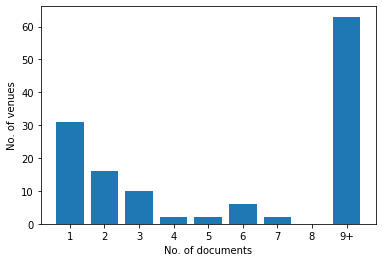
\includegraphics[width=.7\textwidth]{figures/evaluation/docs_per_venue.png}
    \caption{Number of documents per venue}
    \label{fig:docs_per_venue}
\end{figure}

Figure \ref{fig:docs_per_venue} shows the number of documents per venue. Almost half (48 \%) of the venues in our set are assigned to at least nine documents, whereas 23 \% are assigned to only one. These venues that are assigned to only one document are the professors of fields for which there weren't any popular venues in the repositories. Documents are usually only assigned one venue. This is always the case for publications, which are only be published in one place, but not necessarily for theses, which can have multiple advisors or referees. In our evaluation set, only 2 \% of the documents have more than one venue, and never more than two.

\subsubsection{Summary of the evaluation sets} \label{eval_datasets_summary}

After presenting each evaluation set individually, we now look at them as a whole, focusing on their coverage of repositories (table \ref{tab:eval_repo_coverage}) and fields (figure \ref{fig:eval_field_distribution}). We refer to them as the handwritten set, the \acrshort{ddc} set and the venue set for brevity.

The \acrshort{ddc} set covers by far the most documents of all repositories. As shown in table \ref{tab:eval_repo_coverage}, it covers 70 \% of the documents in all three repositories. depositonce is the repository worst represented in this evaluation set, with only 31 \% coverage. The handwritten set covers more than twice as many documents as the venue set. Contrary to the \acrshort{ddc} set, both these sets cover more of depositonce than of any other repository. This is remarkable given that depositonce is a much smaller repository than refubium.

\begin{table}[]
    \centering
    \begin{tabular}{|c|c|c|c|c|}
        \hline
        \textbf{Evaluation set} & \textbf{total} & \textbf{depositonce} & \textbf{edoc} & \textbf{refubium} \\ \hline \hline
        \textbf{Handwritten} & 24 \% & 29 \% & 23 \% & 22 \% \\ \hline
        \textbf{DDC} & 70 \% & 31 \% & 78 \% & 86 \% \\ \hline
        \textbf{Venues} & 11 \% & 16 \% & 14 \% & 8 \% \\ \hline
    \end{tabular}
    \caption{Repository coverage of the evaluation sets.}
    \label{tab:eval_repo_coverage}
\end{table}

Figure \ref{fig:eval_field_distribution} compares the coverage of the \acrshort{mag} fields by the evaluation sets, in percentages. The field percentages of an evaluation set results add up to 100 \%. The \acrshort{ddc} evaluation set is the most polarized of all. 18 \% of its documents belong to the field of \textit{Medicine}, and the fields \textit{Biology}, \textit{Physics} and \textit{Economics} each represent 13 \% of the evaluation set. Thus, 57 \% of the documents of the \acrshort{ddc} evaluation set belong to only four fields, out of 19.

The popularity of \textit{Medicine} in the \acrshort{ddc} set results of its large coverage of refubium (86 \%), which is the largest repository of the three and includes documents from Charité, the Medical University of Berlin. \textit{Economics} is a popular field both in \textit{refubium} and \textit{edoc}, as was discussed in chapter \ref{repo_analysis_subjects}. Furthermore, the \acrshort{ddc} evaluation set does not have any documents of the fields \textit{Materials science}, \textit{Business} and \textit{Environmental science}, as well as barely any belonging to \textit{Art} or \textit{Geography}. Therefore, there are three empty fields and two that are barely represented in this set.

The handwritten set is the most evenly distributed set regarding fields, and is the only one that covers all fields. The fields that stand out the most are \textit{Biology}, which accounts for 12 \% of the documents, followed by \textit{Medicine} and \textit{Physics}, both with 8 \% of the documents. Its worst represented fields are \textit{Business}, \textit{Environmental Science} and \textit{Art}, which are also among the least represented fields of the \acrshort{ddc} set.

The venue set is dominated by depositonce and edoc, which almost double refubium regarding repository coverage. This explains the two most popular fields, which differ from those in the other evaluation sets, as they do not appear often in refubium: \textit{Chemistry} accounts for 13 \% of the documents, and \textit{Computer science}, for 12 \%. On the other hand, this set doesn't have any documents for \textit{Art} and barely any for \textit{Philosophy}, \textit{History}, \textit{Geology}, \textit{Sociology}, \textit{Business} and \textit{Political Science}. These seven fields account for only 4.5 \% of the documents of this evaluation set.

\begin{figure}
    \centering
    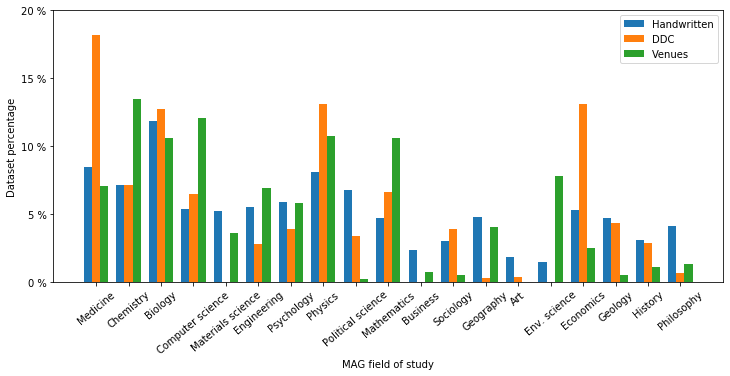
\includegraphics[width=\textwidth]{figures/evaluation/eval_field_distribution.png}
    \caption{Distribution of the evaluation set among the MAG fields of study.}
    \label{fig:eval_field_distribution}
\end{figure}

The natural sciences dominate all evaluation sets. It can be clearly seen in figure \ref{fig:eval_field_distribution}, where the bars to the left are much higher than those to the right. \textit{Medicine}, \textit{Biology} and \textit{Physics} appear more than 1,200 times in all three evaluation sets, mainly due to the \acrshort{ddc} evaluation set, which covers far more documents than the other two sets. On the other end of the spectrum, \textit{Art} and \textit{Business} are the only fields with less than 100 appearances in the evaluation sets. However, the average number of appearances per field exceeds 540 documents.
\subsection{Evaluation metrics} \label{eval_metrics}

In this section, we present evaluation metrics that are commonly used in the literature. Choosing the right metric is very important when measuring the performance of the model. Before doing so, one should first decide which aspects of the use case are the most relevant, as different metrics measure different things. For instance, a model can be highly accurate but output few subjects. Accuracy is more relevant than completeness for some use cases, and in others, it is the other way around.

In section \ref{eval_metrics_flat}, we discuss evaluation metrics that can be used with any set of subjects, whether they have a hierarchy or not. These metrics are binary: an assignment is either right or wrong, there is nothing in between. We then look at metrics that were designed specifically for hierarchical sets of subjects, in section \ref{eval_metrics_hierarchy}. These metrics take into account how far the guessed subjects are from the correct ones, e.g. by looking at their common ancestors in the hierarchy. Such metrics are better suited for hierarchies of subjects, as accuracies can be evaluated more precisely.

Finally, we look at precision-recall curves in section \ref{eval_metrics_curve}. This metric overcomes the issue of picking a threshold value for the assignment probabilities, which is a subjective decision and strongly impacts the performance of the model. For example, for a threshold of 80 \%, we assign all subjects to documents whose probability scores are at least 80 \%. This determines how many subjects are assigned, and affects the performance of the model in the metrics presented in the previous sections.

Once we have presented all these metrics, we pick the ones we find suitable for our approach in section \ref{eval_metrics_our}. We have chosen metrics that consider the incompleteness of our evaluation set, which includes only a few subjects per document, if any.

\subsubsection{Flat metrics} \label{eval_metrics_flat}

Flat evaluation metrics are those that don't consider the hierarchy of the subjects, or any relationship between subjects, for that matter. Each assignment is considered to be either right or wrong. There are two main types of flat metrics \cite{giraldo2015evaluation}:

\begin{enumerate}
    \item \textbf{label-based metrics}, which evaluate the performance for each label (i.e. subject, in our case), and
    \item \textbf{example-based metrics}, which evaluate the performance for each example, which in our case means a document in the evaluation set.
\end{enumerate}

We will look into both families of flat metrics, as well as some of their variations, in the following sections.

\paragraph{Label-based metrics} \mbox{}

The three most common label-based metrics for text classification are precision, recall and the F-score \cite{sebastianini2002machine}. They are all computed with the number of true positives (TP), false positives (FP), true negatives (TN) and false negatives (FN). In our case, a TP is a correctly assigned subject, whereas a FP is an incorrectly assigned subject. Analogously, a TN is a subject that was correctly discarded, and a FN is a subject that is not assigned, but should have been. Thus, \textit{true} and \textit{false} define if the decision has been right or wrong, and \textit{positive} and \textit{negative} express if the subject was assigned or not.

\textit{Precision} ($P$ in the formula below) describes how often assignments are correct. \cite{sebastianini2002machine} refers to precision as the \textit{degree of soundness} of an index. A low precision means that many of the assigned subjects are wrong, whereas a high precision means that few errors were made. It is important to note that this metric does not consider the number of assignments. For example, a model can have perfect precision (i.e. $P=1$) by only assigning one subject to a document. This method is inferior to another method that assigns thousands of subjects, with a lower precision of, say, $P=0.9$. Therefore, precision is usually evaluated together with recall.

$$ P = \frac{TP}{TP + FP} $$

\textit{Recall} ($R$ in the formula below) describes how many of the made assignments are correct, in contrast with how many correct assignments are missing. \cite{sebastianini2002machine} describes recall as the \textit{degree of soundness} of an index, which makes sense looking at the example above: it is not sound, given it has only made one assignment. Even if this single assignment is correct, many other correct assignments are missing.

$$ R = \frac{TP}{TP + FN} $$

Precision and recall are often combined, as they measure two important aspects of the assignments and complement each other very well. The \textit{F-score} combines precision and recall with a parameter $\beta$, which determines the relative importance of them \cite{medelyan2008domain}. $\beta$ is usually set to one, resulting in the harmonic mean of precision and recall, shown in the formula below.

$$ F_1 = 2 \frac{P \cdot R}{P + R} $$

\paragraph{Averaging methods} \mbox{}

The three metrics presented above can be computed in three different ways:

\begin{enumerate}
    \item \textbf{Micro-average}: all results are considered at the same time.
    \item \textbf{Macro-average}: results are grouped by subject.
    \item  \textbf{Sample-based average}: results are grouped by document.
\end{enumerate}

Macro-averaged metrics consider all assignments at once regardless of the subject or the document. The metric is computed once with all assignments. We illustrate this below with the formula for the macro-averaged precision.

$$ P_{macro} = \frac{1}{|S|} \sum_{s \in S} P_s  $$

Micro-averaged metrics, on the other hand, compute the metric for each subject separately, and then average over the results. Below we show the formula for the micro-averaged precision.

$$ P_{micro} = \frac{\sum_{s \in S} TP_s}{\sum_{s \in S} TP_s + FP_s}   $$

Each of these aggregation methods has its advantages and disadvantages: which metric or aggregation method is better depends on the application \cite{toepfer2020fusion}. For instance, the $F_1$-score does not consider TN, as its value is dominated by the number of TP \cite{gargiulo2019deep}. Therefore, smaller classes have little influence in the resulting score when micro-averaging. This is not an issue for use cases where the number of correct assignments matters more than having a consistent performance across labels. On the other hand, macro-averaged results give an equal weight to each class, and is better suited for cases where all subjects are equally important, regardless how often they are assigned to documents.

\paragraph{Example-based metrics} \mbox{}

Example-based metrics, as mentioned at the beginning of this section, evaluate examples of the evaluation set instead of labels. In our case, an example is a document in the evaluation set. Studies indicate that example-based metrics are better suited for multi-label settings, as they consider all subjects simultaneously \cite{giraldo2015evaluation}. Precision, recall and F-scores can also be computed regarding the intersection of the set of predicted subjects $\hat{Y}_d$ with the set of true subjects $Y_d$ \cite{gargiulo2019deep}. For instance, the \textit{example-based precision} ($P_{EB}$ in the formula below), estimates how many predicted labels are correct.

$$ P_{EB} = \frac{1}{|D|} \sum_{d \in D} \frac{|Y_d \cap \hat{Y}_d|}{|Y_d| + |\hat{Y}_d|} $$

\paragraph{Accuracy} \mbox{}

Accuracy does not depend on the micro- or macro-average, and is an alternative to precision and recall \cite{gargiulo2019deep}. However, it is not often used in text classification because the large denominator (the number of subjects) makes this metric insensitive to variations in the number of correct decisions \cite{sebastianini2002machine}. Another issue is that, given that in multi-label settings there are usually many more true negatives than true positives, making no assignments often yields the best accuracy. This does not happen with the F1-score.

$$ Acc = \frac{\sum_{s \in S} \frac{TP_s + TN_s}{TP_s + TN_s + FP_s + FN_s}}{|S|} $$

\subsubsection{Hierarchical metrics} \label{eval_metrics_hierarchy}

Hierarchical metrics are designed specifically for hierarchical sets of subjects. They take into account how far the guessed subjects are from the correct ones, e.g. by looking at their common ancestors in the hierarchy. For example, if a document is assigned the subject \textit{k-nearest neighbors}, which is a clustering algorithm, predicting the subject \textit{neural network} is closer than \textit{urban planning}, although both predictions are wrong. Hierarchical metrics aim to recognize the difference between both predictions, penalizing \textit{urban planning} more than \textit{neural network}.

These metrics assume that the assignments are consistent. If a subject is assigned to a document, all its ancestors in the hierarchy should also be assigned to the same document. In the case of \textit{k-nearest neighbors}, its parents would be \textit{clustering algorithms}, \textit{machine learning} and \textit{computer science}, for example. Precision, recall and F-scores can be adapted to hierarchical structures of subjects by considering the sets of predicted and true labels \cite{gargiulo2019deep}. In fact, they already do so in their example-based formulations, if the assignments are consistent with the hierarchy.

Common ancestors between predicted and true subjects increase the performance of the model in these metrics, as they are all included in the sets of subjects. However, adding all the ancestors can also lead to overestimating errors when the hierarchy has many levels. If assigned subjects have many ancestors, the sets of assigned and predicted subjects will be very large and may differ greatly, even if the predicted and assigned subjects are not so semantically different.

\cite{kosmopoulos2015evaluation} proposes several metrics that, instead of comparing complete sets of subjects, looks for the common ancestors of true and predicted subjects. The \acrfull{lca} of two nodes is the node that is furthest from the root, considering the common ancestors of the two nodes. As we don't know how to map the predicted subjects to the true ones, we consider all true subjects when looking for the \acrshort{lca} of a predicted subject. Thus, each predicted subject is compared to its most similar subject in the true set of subjects. The same is done the other way around, i.e. looking for the \acrshort{lca} for each true subject with the set of predicted subjects. Then we have again two sets of subjects, and the common metrics such as precision, recall and F-scores can be computed.

\subsubsection{Precision-recall curves} \label{eval_metrics_curve}

\acrfull{mlc} models usually output assignment probabilities for the subject, finally assigning those that are above a certain threshold. The choice of a threshold depends on what the assigned subjects are going to be used for. For instance, if one wants to relate documents to one another, a lower threshold will be picked, so that each document has more subjects, which results in more connections to other documents. On the other hand, if wrong predictions are not acceptable, like for example in the biomedical field, a higher threshold would be better.

Therefore, research on \acrshort{mlc} is usually evaluated with precision-recall curves \cite{wehrmann2018hierarchical}, which plot the trade-off between precision and recall for different threshold values (i.e. from zero to one). To enable the comparison between different curves, the area under the curve is measured. which results in a scalar that can be easily compared across methods. A higher area under the curve means that both the recall and the precision are high. Therefore, models with higher areas are considered better.

\subsubsection{Our metrics} \label{eval_metrics_our}

The researchers that use the metrics presented above use complete evaluation sets, where the subjects have been manually assigned to the documents. They are also noisy, given the lack of inter-indexer consistency \cite{csomai2007investigations}, but each document has multiple assigned subjects, which together describe their ``aboutness''. Our evaluation sets, as discussed in section \ref{eval_datasets_summary}, are sparse. They include only a few assignments per document, usually just one and sometimes none. We have to take this aspect into account when picking evaluation metrics.

Here we present the two metrics we use to evaluate the two approaches. The first one, called accuracy, checks if the correct subject is included among the top $n$ subjects output by a given model. The second metric, called \acrfull{lcas}, quantifies the \acrfull{lca} between the correct subject and the top $n$ subjects output by a model. The second metric is only used in the handwritten evaluation set, as the other two evaluation sets only consider fields, which don't have any ancestors.

\paragraph{Hit rate} \mbox{}

\textit{Hit rate} is an intuitive metric that measures how often the correct subject is within the top $n$ candidates output by a model as a percentage. We consider each assignment individually, checking if it is in the list of candidates or not. Then we divide the number of correct inclusions by the number of total checks. If a document has multiple assignments, each are considered independently.

For the \acrshort{ddc} and venue evaluation sets, where there are only 19 possible assignments, the number of candidates ranges from one to five. For the handwritten evaluation set, where there are 2,157 possible assignments, we consider 5, 10, 20, 30 and 50 candidates. Recall that the subject assignments of this dataset are not necessarily those that best represent their respective documents, and therefore are not expected to be on their top 5 or 10 candidates.
 
This metric is analogous to the one used in object recognition tasks in ImageNet \cite{russakovsky2015imagenet}, called \textit{error rate}, where they count misses instead of hits. Considering a variable number of candidates, they measure how often the correct assignments are not included. Thus, a lower error rate is better. In our case, where we count hits, a higher hit rate is better.

\paragraph{LCAS} \mbox{}

The \acrfull{lcas} is based on the evaluation metric proposed in \cite{kosmopoulos2015evaluation}, which quantifies the similarity of two subjects based on their \acrfull{lca}. \cite{kosmopoulos2015evaluation} concludes that a set-based version of the F1-score is the best metric for most use cases, but that pair-based metrics might be better for special cases. As stated above, our evaluation set is special because of its incompleteness. It contains one assignment per document, if any. Therefore, we adapt their metric to our case.

We define this metric by considering a \textit{correct subject}, which is the subject assigned to a document in the evaluation set, and a \textit{candidate subject}, which is the subject assigned to a document by a model. The candidate subject doesn't have to be correct, i.e. it is not always the same as the correct subject. As mentioned above, the \acrshort{lca} of two subjects is the subject that is furthest from the root, considering the common ancestors of the two subjects. We quantify the \acrshort{lca} by measuring the length of the path from the root (i.e. the fields) to the \acrshort{lca}.

Given that the depths of the paths from the fields to the subjects vary depending on the subject, we divide the length of the path to the \acrshort{lca} by the length of the path to the subject. This normalizes the \acrshort{lcas}, so larger paths are not overestimated. We also add one to all paths, which is the same as adding another node above the fields. We do this, so fields don't receive an \acrshort{lcas} of zero, as their actual path length is zero. Furthermore, adding one to all paths avoids divisions by zero if the correct subject is a field.

As correct and candidate subjects may have multiple common ancestors in the same hierarchy level, we always pick the ancestor for which the \acrshort{lcas} is highest. This evaluation metric, as the first one, is parameterized by the number of candidates. The formal definition of the \acrshort{lcas} can be seen below, where $Y$ is the correct subject, $X$ is the candidate subject and $LCA(X,Y)$ is their \acrshort{lca}. $P(S)$ is the path from the root to the subject $S$, and $|P(S)|$ denotes the length of that path.

$$ LCAS(X, Y) = \frac{|P(LCA(X, Y))|+1}{|P(Y)|+1}$$

\paragraph{Example of the LCAS} \mbox{}

\begin{figure}
    \centering
    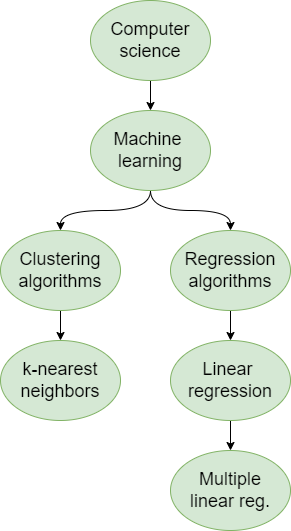
\includegraphics[width=.4\textwidth]{figures/evaluation/subject_hierarchy_example.png}
    \caption{Example of a subject hierarchy}
    \label{fig:subject_hierarchy_example}
\end{figure}

We illustrate the \acrshort{lcas} using the subject hierarchy shown in figure \ref{fig:subject_hierarchy_example}, which comprises subjects of the field \textit{Computer science}, with five hierarchy levels.

For correct subject \textit{Linear regression} and candidate subject \textit{Clustering algorithms}, the \acrshort{lca} would be \textit{Machine learning}. The path from the field \textit{Computer science} to the subject \textit{Linear regression} has length 3, as it passes through \textit{Machine learning} and \textit{Regression algorithms}. The length of the path to the \acrshort{lca} is 1. Thus, the \acrshort{lcas} for subject \textit{Linear regression} and candidate \textit{Clustering algorithms} is $\frac{1}{2}$. We show it in mathematical notation below, with each subject abbreviated to its initials for clarity.

$$ LCAS(CA, LR) = \frac{|P(LCA(CA, LR))|+1}{|P(LR)|+1} = \frac{|P(ML)|+1}{|P(LR)|+1} = \frac{2}{5} = \frac{1}{2} $$

If the correct subject were \textit{Multiple linear regression}, which descends from \textit{Linear regression}, the \acrshort{lcas} would be lower ($\frac{2}{5}$ instead of $\frac{1}{2}$). This is expected, as the descendant is further away from the \acrshort{lca}. On the other hand, if it were \textit{Machine learning}, which is an ancestor of the candidate, the \acrshort{lcas} would be $1$, which is its maximum value. This is also expected as the \acrshort{lca} is \textit{Machine learning} itself. The same \acrshort{lcas} would be achieved if the correct subject were \textit{Computer science}.

\begin{table}[]
    \centering
    \begin{tabular}{|c|c|}
        \hline
        \textbf{Correct subject} & \textbf{LCAS} \\ \hline\hline
        Computer science & 1 \\ \hline
        Machine learning & 1 \\ \hline
        Clustering algorithms & 1 \\ \hline
        k-nearest neighbors & 0.75 \\ \hline
        Regression algorithms & 0.67 \\ \hline
        Linear regression & 0.5 \\ \hline
        Multiple linear reg. & 0.4 \\ \hline
    \end{tabular}
    \caption{LCAS for several subjects where the candidate is \textit{Clustering algorithms}.}
    \label{tab:lcas_example}
\end{table}

In table \ref{tab:lcas_example}, we show several \acrshort{lcas} where \textit{Clustering algorithms} is the candidate subject. Here we can see that the \acrshort{lcas} decreases as we go deeper into the other subtree, and also that it is equal to one, the maximum value, when the correct subject is above the candidate subject in the hierarchy. Another interesting characteristic of the \acrshort{lcas} is that guesses that are further down in the hierarchy are rewarded. Thus, although the relative position of the subjects is the same, being close to a correct subject that is deeper in the hierarchy outputs a higher \acrshort{lcas}. For example, the \acrshort{lcas} of correct subject \textit{Linear regression} and candidate \textit{Regression algorithms} is $0.75$, whereas for correct subject \textit{Multiple linear regression} and candidate \textit{Linear regression}, the \acrshort{lcas} is $0.8$.

\subsection{Results of the unsupervised approach}

In this section, we assess the performance of the unsupervised approach with the evaluation sets. We first confirm the results of our qualitative assessment of the vector combination methods, which indicated that summing the vectors yields better results than averaging or concatenating them. The performance of the sum method on the venue and \acrshort{ddc} evaluation sets is considerably higher than that of the other two methods.

We then evaluate the performance of the sum method in the handwritten evaluation set. Its performance is lower than in the other evaluation sets, where only fields of study are considered. This is to be expected, given that there are 2,157 candidate subjects instead of 19, but it is still low.

We already discussed possible reasons for this difference in performance in section \ref{unsupervised_approach_conclusion}. The main challenge is the size of the dataset. The small amount of relationships that can be built between documents, and also between documents and venues, hinders the representations of the documents.

\subsubsection{Comparing the vector combination methods}

\begin{figure}
  \begin{subfigure}[t]{.45\textwidth}
    \centering
    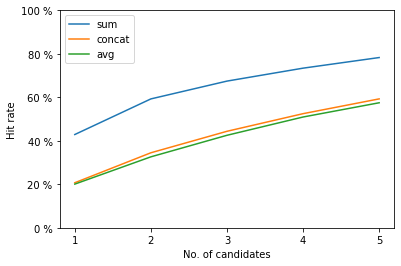
\includegraphics[width=\textwidth]{figures/unsupervised_approach/results/cosine_methods_ddc.png}
    \caption{DDC subjects}
    \label{fig:cosine_methods_ddc}
  \end{subfigure}
  \begin{subfigure}[t]{.45\textwidth}
    \centering
    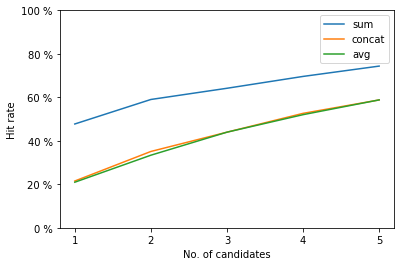
\includegraphics[width=\textwidth]{figures/unsupervised_approach/results/cosine_methods_venues.png}
    \caption{Venues}
    \label{fig:cosine_methods_venues}
  \end{subfigure}
  \caption{Hit rate of the three distance metrics in the evaluation sets.}
  \label{fig:combination_eval}
\end{figure}

We compare the three distance metrics on the two evaluation sets that consider fields, namely the \acrshort{ddc} and the venue evaluation sets. The hit rate of the combination methods is shown in figure \ref{fig:combination_eval}. The sum method outperforms the other two methods by a large margin in both datasets, the difference being usually over 20 \%. The other two methods behave similarly.

The sum method performs better for all considered numbers of candidates. It is also the most efficient, as all objects are represented by 100-dimensional vectors, as well as the only one that doesn't discard any information. The other two methods truncate word vectors, to match the sizes between the representations of documents and subjects.

\subsubsection{Results on the evaluation sets} \label{unsupervised_approach_results_eval}

\begin{figure}
  \begin{subfigure}[t]{.32\textwidth}
    \centering
    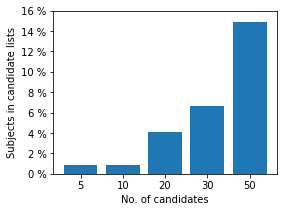
\includegraphics[width=\textwidth]{figures/unsupervised_approach/results/first_hw.png}
    \caption{Handwritten subjects}
    \label{fig:first_hw}
  \end{subfigure}
  \begin{subfigure}[t]{.32\textwidth}
    \centering
    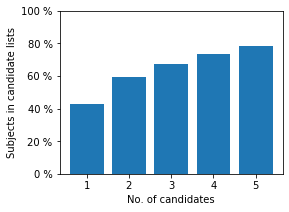
\includegraphics[width=\textwidth]{figures/unsupervised_approach/results/first_ddc.png}
    \caption{DDC subjects}
    \label{fig:first_ddc}
  \end{subfigure}
   \begin{subfigure}[t]{.32\textwidth}
    \centering
    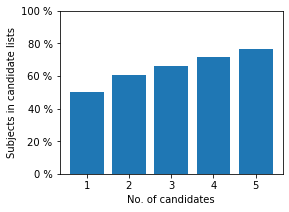
\includegraphics[width=\textwidth]{figures/unsupervised_approach/results/first_venue.png}
    \caption{Venues}
    \label{fig:first_venue}
  \end{subfigure}
  \caption{Hit rate of the unsupervised approach in the evaluation sets.}
  \label{fig:first_eval}
\end{figure}

Here we present the final results of the unsupervised approach, using the sum method as the distance metric. We have computed the distances between the documents and the subjects that descend from the five fields that are the closest to each document. We then store the 50 subjects that are the closest to each document. The hit rate of this approach on the evaluation set is depicted in figure \ref{fig:first_eval}. The hit rate on the \acrshort{ddc} and venue evaluation sets was already shown when comparing the different distance metrics.

The hit rate of this approach on the handwritten set is lower than in the other two datasets. Being accurate is much less likely in this set, as it has 2,157 options instead of 19, so the lower hit rate is to be expected. The hit rate of the model increases dramatically when more candidates are considered, reaching a maximum value of 15 \% when the 50 most similar subjects are considered. Recall that the subjects present in this evaluation set are not necessarily those that describe best the documents they are assigned to. They are merely those that appear in our subset of \acrshort{mag} subjects. Therefore, it is normal that the hit rate is so low when considering small numbers of candidates.

\begin{figure}
    \centering
    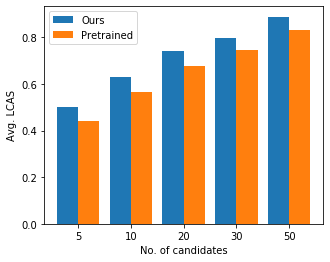
\includegraphics[width=.7\textwidth]{figures/unsupervised_approach/results/avg_lcas.png}
    \caption{Avg. LCAS of the unsupervised approach method, with and without pre-trained embeddings.}
    \label{fig:avg_lcas}
\end{figure}

\begin{figure}
    \centering
    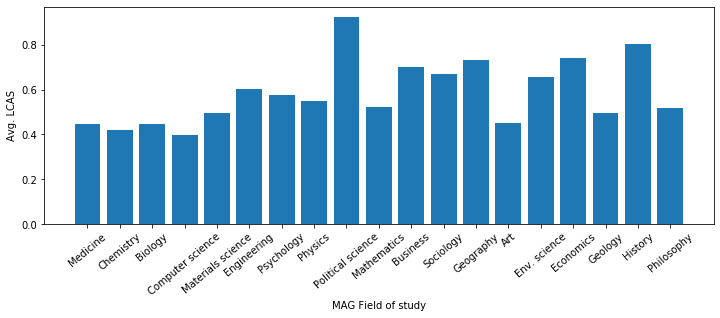
\includegraphics[width=\textwidth]{figures/unsupervised_approach/results/field_lcas.png}
    \caption{Avg. LCAS for each field using the unsupervised approach method and considering five candidates.}
    \label{fig:field_lcas}
\end{figure}

Regarding the \acrfull{lcas}, shown in figure \ref{fig:avg_lcas}, it steadily increases with the number of candidates, reaching a maximum average value of $0.89$. This value is very high, meaning that the guesses are close to the correct subjects in the subject hierarchy. We have also computed the average \acrshort{lcas} for each field, when considering five candidates. This is shown in figure \ref{fig:field_lcas}. \textit{Political Science} has a remarkably high value, over $0.9$, which results of averaging the \acrshort{lcas} of 898 assignments. Apparently, the model is accurately identifying the field.

On the other hand, \textit{Computer science} has a low average \acrshort{lcas} considering how popular the field is in our dataset. It may have to do with the fact that the subjects present in the handwritten set are not the top choices for the indexed documents and therefore do not appear in the top five candidates. When considering 50 candidates, \textit{Computer science} reaches an \acrshort{lcas} of $0.8$, and all other fields over $0.75$

\subsubsection{Using pre-trained embeddings} \label{unsupervised_approach_results_pretrained}

\begin{figure}
  \begin{subfigure}[t]{.32\textwidth}
    \centering
    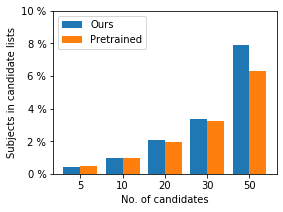
\includegraphics[width=\textwidth]{figures/unsupervised_approach/results/pretrained_hw.png}
    \caption{Handwritten subjects}
    \label{fig:pretrained_hw}
  \end{subfigure}
  \begin{subfigure}[t]{.32\textwidth}
    \centering
    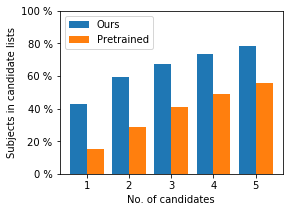
\includegraphics[width=\textwidth]{figures/unsupervised_approach/results/pretrained_ddc.png}
    \caption{DDC subjects}
    \label{fig:pretrained_ddc}
  \end{subfigure}
   \begin{subfigure}[t]{.32\textwidth}
    \centering
    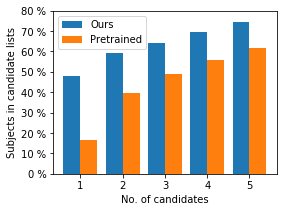
\includegraphics[width=\textwidth]{figures/unsupervised_approach/results/pretrained_venue.png}
    \caption{Venues}
    \label{fig:pretrained_venue}
  \end{subfigure}
  \caption{Hit rate of the unsupervised approach in the evaluation sets, with and without pre-trained embeddings.}
  \label{fig:pretrained_eval}
\end{figure}

Using pre-trained vector embeddings is common practice for \acrfull{nlp} tasks \cite{mikolov2017advances}. Such embeddings are trained on very large corpora and thus more accurately represent their corresponding words. Especially tasks on small datasets benefit from this transfer. However, technical datasets may not benefit as much from such pre-trained embeddings. They include words that are otherwise rare in non-scientific literature, and the style of writing is also different.

Here, we implement the same unsupervised approach, only changing the embeddings used to vectorize the texts. Instead of using the embeddings we have trained on our corpus, we use the pre-trained ones presented in section \ref{supervised_approach_embeddings}. Less than 3 \% of the words of our texts are not present in the file of pre-trained embeddings. If it were more, the lack of coverage would significantly hinder the performance of the method. This could still be the case, if the most distinctive words of each text are the ones missing.

Surprisingly, our own embeddings offer better results on the evaluation datasets, as shown in figure \ref{fig:pretrained_eval}. The method with our embeddings outperforms the one with the pre-trained embeddings on every dataset, for every number of candidates. Especially for the datasets regarding fields, the \acrshort{ddc} and venue datasets, the difference in hit rate is mostly around 30 to 50 \%. In the handwritten set, the difference is not so large, given that both models perform poorly.

This shows that our embeddings do a better job at representing the documents of the repositories. It is surprising that they are so much better, given the small size of our corpus. However, given how technical our corpus is, including fields both from the natural and the social sciences, it is to be expected that pre-trained embeddings don't work as well as in other use cases, where the data is similar to the one used to pre-train the embeddings.

The average \acrshort{lcas} of this method is depicted in figure \ref{fig:field_lcas} for several number of candidates. There it can be seen that using our own embeddings consistently improves the \acrshort{lcas} by $0.1$, which is a significant difference. Still, this method reaches an avg. \acrshort{lcas} of $0.8$ when considering 50 candidates.

\subsection{Results of the supervised approach} \label{results_supervised}

\begin{figure}
  \begin{subfigure}[t]{.5\textwidth}
    \centering
    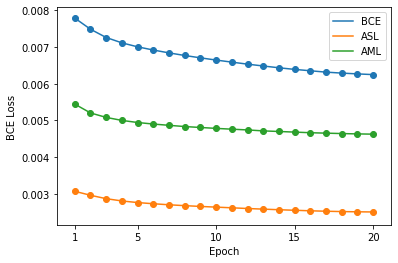
\includegraphics[width=\textwidth]{figures/supervised_approach/all_train_loss.png}
    \caption{Training loss}
    \label{fig:all_train_loss}
  \end{subfigure}
   \begin{subfigure}[t]{.5\textwidth}
    \centering
    \includegraphics[width=\textwidth]{figures/supervised_approach/all_test_loss.png}
    \caption{Testing loss}
    \label{fig:all_test_loss}
  \end{subfigure}
  \caption{Test and training loss of the three final models.}
  \label{fig:all_train}
\end{figure}

\begin{figure}
  \begin{subfigure}[t]{.32\textwidth}
    \centering
    \includegraphics[width=\textwidth]{figures/supervised_approach/all_hw.png}
    \caption{Handwritten subjects}
    \label{fig:all_hw}
  \end{subfigure}
  \begin{subfigure}[t]{.32\textwidth}
    \centering
    \includegraphics[width=\textwidth]{figures/supervised_approach/all_ddc.png}
    \caption{DDC subjects}
    \label{fig:all_ddc}
  \end{subfigure}
   \begin{subfigure}[t]{.32\textwidth}
    \centering
    \includegraphics[width=\textwidth]{figures/supervised_approach/all_venue.png}
    \caption{Venues}
    \label{fig:all_venue}
  \end{subfigure}
  \caption{Hit rate of the three final models for the evaluation sets.}
  \label{fig:all_eval}
\end{figure}

Now we compare the three supervised models presented in section \ref{supervised_approach_models}, each with a different loss function: the \acrshort{bce} model, the \acrshort{asl} model and the \acrshort{aml} model. We use the best models that result from the experiments, presented in appendix \ref{supervised_approach_experiments}, and train them for an additional 20 epochs.

The testing loss of the \acrshort{bce} model is significantly lower, whereas the other two testing losses are similar, as shown in figure \ref{fig:all_train}. The training losses are very similar for all three models, differing in the thousandths. The training loss of the \acrshort{bce} model decreases the most out of the losses of the three models. On the other hand, the testing losses remained very steady for all three models. The \acrshort{asl} model seems to have benefitted the most from the additional training.

The \acrshort{bce} model yields the best hit rate on all three evaluation sets, as can be seen in figure \ref{fig:all_eval}, as well as the best \acrshort{lcas}, shown in figure \ref{fig:all_lcas}. The difference in hit rate to the other models is consistently around two percentage points throughout all numbers of candidates. The \acrshort{aml} model outperforms the \acrshort{asl} model on the handwritten evaluation set.  However, the \acrshort{asl} model has a better \acrshort{lcas}, meaning that its guesses are overall better than those of the \acrshort{aml} model. Furthermore, it performs better on the \acrshort{ddc} evaluation set. Still, both models don't perform as well as the \acrshort{bce} model. This could be because the model parameters and the training settings were optimized for that model, and the further extensions introduced by the other two models required other values for those parameters.

\begin{figure}
    \centering
    \includegraphics[width=.6\textwidth]{figures/evaluation/all_lcas.png}
    \caption{LCAS comparison of the three models.}
    \label{fig:all_lcas}
\end{figure}
\subsection{Comparison of the approaches} \label{results_final}

\begin{figure}
  \begin{subfigure}[t]{.32\textwidth}
    \centering
    \includegraphics[width=\textwidth]{figures/supervised_approach/compare_hw.png}
    \caption{Handwritten subjects}
    \label{fig:compare_hw}
  \end{subfigure}
  \begin{subfigure}[t]{.32\textwidth}
    \centering
    \includegraphics[width=\textwidth]{figures/supervised_approach/compare_ddc.png}
    \caption{DDC subjects}
    \label{fig:compare_ddc}
  \end{subfigure}
   \begin{subfigure}[t]{.32\textwidth}
    \centering
    \includegraphics[width=\textwidth]{figures/supervised_approach/compare_venue.png}
    \caption{Venues}
    \label{fig:compare_venue}
  \end{subfigure}
  \caption{Hit rate of the approaches for the evaluation sets.}
  \label{fig:compare_eval}
\end{figure}

\begin{figure}
    \centering
    \includegraphics[width=.6\textwidth]{figures/evaluation/compare_lcas.png}
    \caption{LCAS comparison of the approaches.}
    \label{fig:compare_lcas}
\end{figure}

In this section, we compare the unsupervised approach with the best performing supervised model, i.e. the \acrshort{bce} model. We refer to them as \acrfull{um} and \acrfull{sm}, respectively. The \acrshort{sm} outperforms the \acrshort{um} in all evaluation sets, as shown in figure \ref{fig:compare_eval}. The \acrshort{sm} is better at identifying fields than the \acrshort{um}. It performs consistently better on the \acrshort{ddc} and venue evaluation sets. However, the difference in hit rate is the largest for the handwritten set.

Only in the venue set for one candidate does the \acrshort{um} perform better, by a margin of 2 \%. For all other number of candidates, the \acrshort{sm} performs better, by a margin from 8 to 11 \%. The differences on the \acrshort{ddc} set are similar. The difference in performance when identifying all 2,157 subjects is much larger, also in favor of the \acrshort{sm}. The difference between them goes from 8 \% when 5 candidates are considered, to 36 \% for 50 candidates.

The superiority of the \acrshort{sm} on the handwritten set is also confirmed by the \acrshort{lcas}, shown in figure \ref{fig:compare_lcas}. Given the large difference in hit rate between the models, this result is to be expected. However, that the \acrshort{lcas} difference is smaller than the difference in hit rate indicates that the guesses of the \acrshort{um} are close to the correct subjects. This hypothesis is also supported by the high hit rate of the \acrshort{um} when identifying fields in the other two evaluation sets.
\subsection{Impact of document length on hit rate} \label{results_length}

\begin{figure}
  \begin{subfigure}[t]{.32\textwidth}
    \centering
    \includegraphics[width=\textwidth]{figures/supervised_approach/sm_hw_length.png}
    \caption{Handwritten subjects}
    \label{fig:sm_hw_length}
  \end{subfigure}
  \begin{subfigure}[t]{.32\textwidth}
    \centering
    \includegraphics[width=\textwidth]{figures/supervised_approach/sm_ddc_length.png}
    \caption{DDC subjects}
    \label{fig:sm_ddc_length}
  \end{subfigure}
   \begin{subfigure}[t]{.32\textwidth}
    \centering
    \includegraphics[width=\textwidth]{figures/supervised_approach/sm_venue_length.png}
    \caption{Venues}
    \label{fig:sm_venue_length}
  \end{subfigure}
  \caption{Hit rate of the approaches for the evaluation sets, grouped by representation length. We consider 20 candidates for the handwritten set, and 1 for the two others.}
  \label{fig:sm_eval_length}
\end{figure}

In this section, we analyze how the length of the documents affects the hit rate of the \acrshort{sm}, our most accurate model. We already showed the representation lengths of the documents after mapping their tokens to the pre-trained vectors in figure \ref{fig:sm_doc_length}. Over 8,000 documents were represented by less than 50 word vectors, and over 6,000 documents have less than 100 vectors. Here, we compute the accuracies on the evaluation set for each length group.

Figure \ref{fig:sm_eval_length} shows the accuracies of the \acrshort{sm} on the evaluation sets for the different length groups. In contrast to the other figures displaying model hit rate, here the number of candidates is fixed. Instead of considering all documents at once, we compute the hit rate for each length group. The hit rate for documents with less than 50 tokens is significantly worse than for documents with more than 50 tokens. The difference in the \acrshort{ddc} and venue sets between the shortest documents and the rest ranges between 15 and 20 \% for the most part. For the handwritten set, the difference is even larger: between 20 and 25 \%. This shows that the model's hit rate is considerably hindered when the representation of the document comprises less than 50 vectors.

The hit rate of the model steadily increases with longer representations, but at a much lower rate. Recall that representations with more than 250 tokens are truncated; only the first 250 tokens are fed to the model. We thus conclude that the representation length does impact the hit rate of the model. Documents represented with less than 50 documents are especially challenging for the model. If we discarded these documents, the hit rate of the model would increase by at least 20 \% on all evaluation sets.

\subsection{Conclusion} \label{supervised_approach_conclusion}

We conclude this chapter by discussing the complexity of the implementation and some aspects of the model that may be improved to increase the performance of the model. The implementation of the models, as well as gathering the training data, is easy to develop. On the other hand, processing the training data training the models is computationally expensive.

We propose several improvements, mostly regarding the fact that the subject assignments are performed by an algorithm and not by a human. This means that its assignment noise could be modeled more easily, as the algorithms operates in a deterministic manner, whereas humans are not so consistent. Also, the assignment algorithm outputs confidence scores, which could also be used to improve the training procedure.

\subsubsection{Implementation}

The supervised approach was easy to implement. Gathering the training data didn't pose any difficulties because of the \acrshort{api} provided by OpenAlex. We vectorized the data in the same way we vectorized the documents of the repositories. Implementing the model also didn't pose any major challenges, as we used the architecture of related work \cite{gargiulo2019deep}. The further two papers we have implemented extended this initial model, both by modifying the loss function and one with an additional layer. Thus, the implementation time was much shorter than that of the unsupervised approach, which included numerous steps. On the other hand, this approach required training many models, which is computationally expensive. Processing the training data is also expensive.

\subsubsection{Room for improvement}

The hit rate of this approach can be easily improved by gathering more training data. Also, there are many techniques regarding the design and training of neural networks that may be experimented with, such as introducing batch or layer normalization \cite{ba2016layer}. Furthermore, there are two aspects from our use case that we have not considered:

\begin{enumerate}
    \item \textbf{Noise distribution}: model noise can be better modeled than human noise, because it is deterministic. Doing so would increase the performance of the model.
    \item \textbf{Confidence scores}: models output confidence scores for the subject assignments, which could be included in the training procedure, e.g. as a replacement of binary labels.
\end{enumerate}

Both aspects derive from the nature of our training dataset, which was created by an algorithm rather than by humans. Addressing these two points could lead to further improvements in the performance of the model. Label noise is a common topic in the literature, as it is present in all datasets labeled by humans because of their inconsistency (\cite{morris2010individual}, \cite{medelyan2008domain}). Deep networks must handle noise appropriately because, if not, they may overfit on the corrupted labels \cite{chen2019understanding}. There are three ways of handling noise \cite{karimi2020deep}: through the selection of the model and the loss function, by cleaning the data, or by developing a model that models label noise.

We have performed several data cleaning tasks, such as checking the language of the texts (see section \ref{repo_analysis_data}). Furthermore, the \acrlong{asl} models label noise better than \acrlong{bce}, as noise is not symmetric across positive and negative samples, given that positive ones are sparse \cite{zhao2021evaluating}. Still, modeling label noise may further increase the performance of the model, as our training data is estimated to have an assignment accuracy of 80 \% \cite{shen2018web}.

Confidence scores could be used instead of binary labels while training the models. This may help the model assess which subjects are closer thematically to the document. However, it may also introduce more noise.

\pagebreak
\bibliographystyle{acm}
\bibliography{references}
\pagebreak

\begin{appendices}
    \section{Vocabulary with n-grams of up to length 4} \label{appendix_ngram_vocab}

Entries of the vocabulary are extracted from the text as n-grams, which are sequences of tokens of length $n$. To decide on the maximum length of the n-grams we want to extract, we have a look at an existing scientific vocabulary, EuroSciVoc\footnote{\url{https://op.europa.eu/en/web/eu-vocabularies/euroscivoc}}. It contains around a 1,000 scientific fields in several European languages. Including synonyms and related fields of studies, there are 3,494 entries in the vocabulary. 38 \% of them consist of one word and 50 \% of them comprise two words. Only 8 entries are longer than four words.

Given the importance of disposing of a thorough vocabulary, we will keep all n-grams up to those of length four. The ones that only occur once in the corpus will be removed at the end, as they cannot be used to relate documents. We also discard n-grams that contain a punctuation sign that signifies a break in the sentence (i.e. one of these: ``.'', ``,'', ``?'', ``!''). Such n-grams don't form valid phrases.

All n-grams of lengths 2 to 4 amount to many entries in the vocabulary. To reduce its size, we implemented a thorough filtering procedure that removes all entries that are redundant. This procedure is detailed in the following section. Afterwards, we present the resulting vocabulary, before and after filtering. Then, we briefly talk about the execution time of the filtering procedure.


\subsection{Vocabulary filtering} \label{vocab_filtering_ngrams}

Once the vocabulary has been created, we remove the entries that occur in only one document, as they cannot be used to relate documents. We also remove the entries that occur in more than 1,000 documents. We assume that their meanings are too broad and that they are thus not relevant for the task of subject indexing. Entries that are either stop words\footnote{For this purpose, we use NLTK's list of English stop words, which comprises 179 words as of 07/07/2021.} or punctuation signs are also discarded. This is the first step out of four that comprise our filtering procedure.

We remove entries that appear as many times (step 2) or one time more (step 3) than entries that contain them, as they only provide meaning when used with other words. For example, if ``supervised'' and ``supervised learning'' both occur 100 times, ``supervised'' should be removed. Also, if ``supervised'' occurs 101 times it should also be removed, as it only occurs once without being in ``supervised learning'' and thus belongs to the set of entries that cannot be used to relate documents.

Lastly, on step 4, we remove entries that either never occur alone or only once. For each entry, we find all the entries that include it. If the sum of their frequencies equals the frequency of the entry or is off by one (i.e. one less), we remove the entry. For example, if ``learning'' appears 100 times, ``supervised learning'' appears 40 times and ``machine learning'' appears 60 times, ``learning'' never occurs alone and should be removed. This step is computationally much more costly than the previous one, as all the remaining entries must be checked. This is why it is performed last.

It is important to note that the matches between entries are performed on the basis of tokens, not raw strings. The latter could lead to spurious behavior such as removing ``selling'' because it occurs as many times as ``counselling'', although they are different words.

\subsection{Resulting vocabulary}

In this section, we will present some facts about the vocabulary that arises from the procedure described above. We first look at the vocabulary before applying the filtering procedure described in section \ref{vocab_filtering_ngrams}, then look at its impact and the final vocabulary.

\subsubsection{Before filtering}

Before filtering, there are 8,892,623 entries in the vocabulary. As shown in figure \ref{fig:vocab_before_words}, almost half of them comprise four words (46 \%), while more than a third (36 \%) comprise three words. 15 \% of them consist of two words and 1.4 \% of them are singular words. This distribution makes sense, as there are fewer duplicates in larger n-grams than in singular words.

\begin{figure}
  \begin{subfigure}[t]{0.45\textwidth}
    \centering
    \includegraphics[width=\textwidth]{figures/vocab/before/n_words.PNG}
    \caption{No. of entries per no. of words.}
    \label{fig:vocab_before_words}
  \end{subfigure}
  \hfill
  \begin{subfigure}[t]{0.48\textwidth}
    \centering
    \includegraphics[width=\textwidth]{figures/vocab/before/entry_frequency.PNG}
    \caption{No. of entries per frequency (i.e. in how many documents they appear).}
    \label{fig:vocab_before_freq}
  \end{subfigure}
  \caption{Charts about the vocabulary before filtering.}
\end{figure}

87 \% of them appear only in one document, as illustrated in figure \ref{fig:vocab_before_freq}. 94 \% of the entries that comprise four words occur only once, while only 60 \% of the entries that are singular words are used in only one document. Entries with two and three words occur only once in 71 \% and 86 \% of the time. These percentages are inversely proportional to the number of entries per number of words that the entry has. This also makes sense, given that 4-grams rarely occur more than once (i.e. only when there is an actual scientific term that is this long or if there is a common sequence of four words, such as ``as well as the'', which occurs in 1,132 documents.).

There are 733 entries that occur in more than 1,000 documents. 487 of them (66 \%) comprise only one word. Only one of these entries consists of four words. The list includes words such as ``common'', ``research'' and ``thesis''. These words, although meaningful, occur too often in our dataset to be of any use for the task of semantically relating documents.

\subsubsection{After filtering}

The filtering procedure reduced the size of the vocabulary from 8,892,623 to 754,889 entries. The first step, in which the entries that occur either in one or in more than 1,000 documents are removed, had the largest effect, removing 7,720,983 entries. All but 733 of them are entries that occur only in one document, as was stated in the previous section.

Step 1 is also the only step in which 4-grams were removed, as shown in figure \ref{fig:words_per_entry_per_step}. As 4-grams are the largest n-grams in our dataset, they are not included in any other n-grams and thus cannot be removed by any of the following steps. No entries were removed during step 3, where entries that occurred once more than larger entries that contained them were filtered. This step is therefore not shown in the figures \ref{fig:words_per_entry_per_step} and \ref{fig:avg_frequency_per_step}. 

Figure \ref{fig:avg_frequency_per_step} shows the average frequency of the entries before the filtering procedure and after each step. The avg. frequency increased dramatically after step 1, where all the entries that only appear in one document (which comprise 87 \% of all entries) were removed. After step 4 the average frequency is 4.2, meaning that entries appear on average in around four documents.

Figures \ref{fig:vocab_after_words} and \ref{fig:vocab_after_freq} are equivalent to figures \ref{fig:vocab_before_words} and \ref{fig:vocab_before_freq} but for the filtered vocabulary. Figure \ref{fig:vocab_after_words} shows how the proportion of 4-grams has decreased, whereas the proportion of 2-grams has increased. Figure \ref{fig:vocab_after_freq} no longer includes entries that occur in only one document, as these were removed in step 1 of the filtering procedure. Almost 60 \% of the entries of the filtered vocabulary appear in two documents, while 18 \% appear in five or more documents.

\subsubsection{Execution time of the filtering procedure}

Regarding the performance of the filtering procedure, the first step is by far the fastest, taking only a couple of seconds. Steps 2 and 3 took around two days each, as the entries are grouped by frequency and each entry has to be compared with all the entries in their group. Step 3 took around eight hours less than step 2, as all the entries removed in step 2 were no longer considered. Step 4 took more than six days, as all entries are considered, not only the ones that belong to the same group.

\begin{figure}
  \begin{subfigure}[t]{0.5\textwidth}
    \centering
    \includegraphics[width=\textwidth]{figures/vocab/after/words_per_entry_per_step.PNG}
    \caption{No. of entries per no. of words for each step.}
    \label{fig:words_per_entry_per_step}
  \end{subfigure}
  \hfill
  \begin{subfigure}[t]{0.48\textwidth}
    \centering
    \includegraphics[width=\textwidth]{figures/vocab/after/avg_frequency_per_step.PNG}
    \caption{Avg. frequency of the entries after each step.}
    \label{fig:avg_frequency_per_step}
  \end{subfigure}
  \caption{Charts about the steps of the vocabulary filtering procedure.}
\end{figure}

\begin{figure}
  \begin{subfigure}[t]{0.52\textwidth}
    \centering
    \includegraphics[width=\textwidth]{figures/vocab/after/words_per_entry.PNG}
    \caption{No. of entries per no. of words.}
    \label{fig:vocab_after_words}
  \end{subfigure}
  \hfill
  \begin{subfigure}[t]{0.44\textwidth}
    \centering
    \includegraphics[width=\textwidth]{figures/vocab/after/entry_frequency.PNG}
    \caption{No. of entries per frequency (i.e. in how many documents they appear).}
    \label{fig:vocab_after_freq}
  \end{subfigure}
  \caption{Charts about the vocabulary after filtering.}
\end{figure}

\subsubsection{Quality of the vocabulary}

We have qualitatively assessed how useful the n-grams of the vocabulary are for our task. Unfortunately, most of the ones we have evaluated are uninformative. They are sequences of words that are often written together, but that don't have any special meaning. Examples of these are ``more general question'' and ``discuss the following''. We therefore discard them altogether, given that they dramatically increase the size of the vocabulary.
    \section{Mapping of venues to MAG fields} \label{appendix_venue_map}

Tables \ref{tab:venue_field_map_1}, \ref{tab:venue_field_map_2}, \ref{tab:venue_field_map_3} and \ref{tab:venue_field_map_4} show which venues from the repositories were used to create the venue evaluation dataset, and to which MAG field they are mapped to. The names of people are advisors or referees, which are the equivalent of venues for theses. The table also shows how many documents are assigned each venue. Please note that the venues are input by hand by the users that upload the documents, which is why some of them appear multiple times with different casing. Some names of venues have been shortened for clarity.

\begin{table}
\centering
\begin{tabular}{|c|c|c|}
\hline
\thead{MAG field} & \thead{Venue} & \thead{\# docs} \\
\hline\hline
\multirow{5}{*}{Medicine}
& Journal of Clinical Medicine & 40 \\ \cline{2-3}
& Frontiers in Physiology & 56 \\ \cline{2-3}
& Frontiers in Immunology & 86 \\ \cline{2-3}
& Frontiers in Neurology & 44 \\ \cline{2-3}
& Volk, Hans-Dieter & 38 \\ \cline{2-3}
\hline
\multirow{9}{*}{Chemistry}
& Physical chemistry, chemical physics & 78 \\ \cline{2-3}
& Journal of Chemical Physics & 68 \\ \cline{2-3}
& Clinical Chemistry and Laboratory Medicine & 32 \\ \cline{2-3}
& Molecules & 59 \\ \cline{2-3}
& Freund, Hans-Joachim & 42 \\ \cline{2-3}
& Prof. Dr. Udo Heinemann & 49 \\ \cline{2-3}
& Prof. Dr. Rainer Haag & 65 \\ \cline{2-3}
& Schlögl, Robert & 70 \\ \cline{2-3}
& Schomäcker, Reinhard & 76 \\ \cline{2-3}
\hline
\multirow{9}{*}{Biology}
& Frontiers in Neurology & 44 \\ \cline{2-3}
& Frontiers in Plant Science & 30 \\ \cline{2-3}
& Nucleic Acids Research & 30 \\ \cline{2-3}
& Frontiers in Microbiology & 59 \\ \cline{2-3}
& Microorganisms & 41 \\ \cline{2-3}
& Neubauer, Peter & 80 \\ \cline{2-3}
& Lauster, Roland & 91 \\ \cline{2-3}
& Prof. Dr. Hans Lehrach & 33 \\ \cline{2-3}
& Saumweber, Harald & 34 \\ \cline{2-3}
\hline
\multirow{9}{*}{Computer science}
& Procedia Computer Science & 43 \\ \cline{2-3}
& Informatik-Berichte & 49 \\ \cline{2-3}
& Proc. of the 7th Int. Conf. of EUIS & 104 \\ \cline{2-3}
& Int. Conf. on DC and Metadata Applications & 32 \\ \cline{2-3}
& Müller, Klaus-Robert & 82 \\ \cline{2-3}
& Obermayer, Klaus & 69 \\ \cline{2-3}
& Wolisz, Adam & 46 \\ \cline{2-3}
& Albayrak, Sahin & 46 \\ \cline{2-3}
& Feldmann, Anja & 52 \\ \cline{2-3}
\hline
\multirow{6}{*}{Materials science}
& Soft matter & 49 \\ \cline{2-3}
& Materials & 47 \\ \cline{2-3}
& Journal of Materials Science & 3 \\ \cline{2-3}
& Gurlo, Aleksander & 10 \\ \cline{2-3}
& Auhl, Dietmar & 3 \\ \cline{2-3}
& Banhart, John & 40 \\ \cline{2-3}
\hline
\end{tabular}
\caption{Mapping of venues to MAG fields for the venue evaluation dataset (part 1).}
\label{tab:venue_field_map_1}
\end{table}

\begin{table}
\centering
\begin{tabular}{|c|c|c|}
\hline
\thead{MAG field} & \thead{Venue} & \thead{\# docs} \\
\hline\hline
\hline
\multirow{6}{*}{Engineering}
& Materials & 47 \\ \cline{2-3}
& Sensors & 43 \\ \cline{2-3}
& Applied Sciences & 38 \\ \cline{2-3}
& 11th Global Conf. on Sustainable Manufacturing & 53 \\ \cline{2-3}
& Paschereit, Christian Oliver & 59 \\ \cline{2-3}
& Petermann, Klaus & 49 \\ \cline{2-3}
\hline
\multirow{7}{*}{Psychology}
& Frontiers in Psychiatry & 35 \\ \cline{2-3}
& Frontiers in psychology & 41 \\ \cline{2-3}
& Frontiers in Psychology & 120 \\ \cline{2-3}
& Frensch, Peter A. & 5 \\ \cline{2-3}
& Beyer, Reinhard & 1 \\ \cline{2-3}
& Rolfs, Martin & 6 \\ \cline{2-3}
& Kathmann, Norbert & 9 \\ \cline{2-3}
\hline
\multirow{7}{*}{Physics}
& Physical chemistry, chemical physics & 78 \\ \cline{2-3}
& Journal of Chemical Physics & 68 \\ \cline{2-3}
& New Journal of Physics & 42 \\ \cline{2-3}
& Applied Physics Letters & 67 \\ \cline{2-3}
& Knorr, Andreas & 77 \\ \cline{2-3}
& Elsässer, Thomas & 33 \\ \cline{2-3}
& Benson, Oliver & 57 \\ \cline{2-3}
\hline
\multirow{6}{*}{Political science}
& Prof. Dr. Tanja Anita Börzel, Freie Universität Berlin & 1 \\ \cline{2-3}
& Harders, Cilja & 2 \\ \cline{2-3}
& Prof. Dr. Sabine Kropp & 2 \\ \cline{2-3}
& Mayer, Margit & 1 \\ \cline{2-3}
& Prof. Dr. Thomas Meyer & 1 \\ \cline{2-3}
& von Steinsdorff, Silvia & 1 \\ \cline{2-3}
\hline
\multirow{11}{*}{Mathematics}
& Preprints aus dem Institut für Mathematik & 314 \\ \cline{2-3}
& Okhrin, Ostap & 31 \\ \cline{2-3}
& Bank, Peter & 13 \\ \cline{2-3}
& Blath, Jochen & 9 \\ \cline{2-3}
& Bobenko, Alexander & 4 \\ \cline{2-3}
& Bürgisser, Peter & 6 \\ \cline{2-3}
& Deuschel, Jean-Dominique & 7 \\ \cline{2-3}
& Emmrich, Etienne & 2 \\ \cline{2-3}
& Mehl, Christian & 3 \\ \cline{2-3}
& Scheutzow, Michael & 22 \\ \cline{2-3}
& Steidl, Gabriele & 3 \\ \cline{2-3}
\hline
\end{tabular}
\caption{Mapping of venues to MAG fields for the venue evaluation dataset (part 2).}
\label{tab:venue_field_map_2}
\end{table}

\begin{table}
\centering
\begin{tabular}{|c|c|c|}
\hline
\thead{MAG field} & \thead{Venue} & \thead{\# docs} \\
\hline\hline
\multirow{6}{*}{Engineering}
& Materials & 47 \\ \cline{2-3}
& Sensors & 43 \\ \cline{2-3}
& Applied Sciences & 38 \\ \cline{2-3}
& 11th Global Conf. on Sustainable Manufacturing & 53 \\ \cline{2-3}
& Paschereit, Christian Oliver & 59 \\ \cline{2-3}
& Petermann, Klaus & 49 \\ \cline{2-3}
\hline
\multirow{7}{*}{Psychology}
& Frontiers in Psychiatry & 35 \\ \cline{2-3}
& Frontiers in psychology & 41 \\ \cline{2-3}
& Frontiers in Psychology & 120 \\ \cline{2-3}
& Frensch, Peter A. & 5 \\ \cline{2-3}
& Beyer, Reinhard & 1 \\ \cline{2-3}
& Rolfs, Martin & 6 \\ \cline{2-3}
& Kathmann, Norbert & 9 \\ \cline{2-3}
\hline
\multirow{7}{*}{Physics}
& Physical chemistry, chemical physics & 78 \\ \cline{2-3}
& Journal of Chemical Physics & 68 \\ \cline{2-3}
& New Journal of Physics & 42 \\ \cline{2-3}
& Applied Physics Letters & 67 \\ \cline{2-3}
& Knorr, Andreas & 77 \\ \cline{2-3}
& Elsässer, Thomas & 33 \\ \cline{2-3}
& Benson, Oliver & 57 \\ \cline{2-3}
\hline
\multirow{6}{*}{Political science}
& Prof. Dr. Tanja Anita Börzel, FU Berlin & 1 \\ \cline{2-3}
& Harders, Cilja & 2 \\ \cline{2-3}
& Prof. Dr. Sabine Kropp & 2 \\ \cline{2-3}
& Mayer, Margit & 1 \\ \cline{2-3}
& Prof. Dr. Thomas Meyer & 1 \\ \cline{2-3}
& von Steinsdorff, Silvia & 1 \\ \cline{2-3}
\hline
\multirow{11}{*}{Mathematics}
& Preprints aus dem Institut für Mathematik & 314 \\ \cline{2-3}
& Okhrin, Ostap & 31 \\ \cline{2-3}
& Bank, Peter & 13 \\ \cline{2-3}
& Blath, Jochen & 9 \\ \cline{2-3}
& Bobenko, Alexander & 4 \\ \cline{2-3}
& Bürgisser, Peter & 6 \\ \cline{2-3}
& Deuschel, Jean-Dominique & 7 \\ \cline{2-3}
& Emmrich, Etienne & 2 \\ \cline{2-3}
& Mehl, Christian & 3 \\ \cline{2-3}
& Scheutzow, Michael & 22 \\ \cline{2-3}
& Steidl, Gabriele & 3 \\ \cline{2-3}
\hline
\end{tabular}
\caption{Mapping of venues to MAG fields for the venue evaluation dataset (part 3).}
\label{tab:venue_field_map_3}
\end{table}

\begin{table}
\centering
\begin{tabular}{|c|c|c|}
\hline
\thead{MAG field} & \thead{Venue} & \thead{\# docs} \\
\hline\hline
\multirow{9}{*}{Business}
& Adam, Tim & 4 \\ \cline{2-3}
& Brüggemann, Ulf & 1 \\ \cline{2-3}
& Bruche, Max & 1 \\ \cline{2-3}
& Gassen, Joachim & 9 \\ \cline{2-3}
& Guhl, Daniel & 1 \\ \cline{2-3}
& Klapper, Daniel & 6 \\ \cline{2-3}
& Schöttner, Anja & 1 \\ \cline{2-3}
& Raithel, Sascha & 1 \\ \cline{2-3}
& Prof. Dr. Dietrich Haase & 3 \\ \cline{2-3}
\hline
\multirow{8}{*}{Sociology}
& Blokland, Talja & 6 \\ \cline{2-3}
& Fasang, Anette & 2 \\ \cline{2-3}
& Mau, Steffen & 1 \\ \cline{2-3}
& Prof. Dr. Katharina Bluhm & 2 \\ \cline{2-3}
& Prof. Dr. Sérgio Costa & 3 \\ \cline{2-3}
& Ehlert, Martin & 1 \\ \cline{2-3}
& Prof. Dr. Dieter Ohr & 2 \\ \cline{2-3}
& Prof. Dr. Christian von Scheve & 2 \\ \cline{2-3}
\hline
\multirow{8}{*}{Geography}
& Remote Sensing & 58 \\ \cline{2-3}
& Water & 61 \\ \cline{2-3}
& Dransch, Doris & 3 \\ \cline{2-3}
& Lakes, Tobia & 15 \\ \cline{2-3}
& Lenz, Barbara & 3 \\ \cline{2-3}
& Kulke, Elmar & 4 \\ \cline{2-3}
& Schneider, Christoph & 7 \\ \cline{2-3}
& Rost, Tilmann & 1 \\ \cline{2-3}
\hline
\multirow{4}{*}{Env. science}
& Berlin Conf. on Human Dim. of Global Env. Change & 208 \\ \cline{2-3}
& Berlin conference on global environmental change & 75 \\ \cline{2-3}
& Scherer, Dieter Ernst & 2 \\ \cline{2-3}
& Scherer, Dieter & 9 \\ \cline{2-3}
\hline
\multirow{12}{*}{Economics}
& Edenhofer, Ottmar & 67 \\ \cline{2-3}
& Burda, Prof. Michael C. & 1 \\ \cline{2-3}
& Burda, Michael C. & 16 \\ \cline{2-3}
& Burda, Michael & 10 \\ \cline{2-3}
& Burda, Michael Christopher & 2 \\ \cline{2-3}
& Engelmann, Dirk & 1 \\ \cline{2-3}
& Fratzscher, Marcel & 9 \\ \cline{2-3}
& Greven, Sonja & 3 \\ \cline{2-3}
& Prof. Dr. Roland Strausz & 2 \\ \cline{2-3}
& Prof. Dieter Nautz & 2 \\ \cline{2-3}
& Danzer, Natalia & 1 \\ \cline{2-3}
& Prof. Dr. Dr, Giacomo Corneo & 1 \\ \cline{2-3}
\hline
\end{tabular}
\caption{Mapping of venues to MAG fields for the venue evaluation dataset (part 4).}
\label{tab:venue_field_map_4}
\end{table}

\begin{table}
\centering
\begin{tabular}{|c|c|c|}
\hline
\thead{MAG field} & \thead{Venue} & \thead{\# docs} \\
\hline\hline
\multirow{11}{*}{Geology}
& Krawczyk, Charlotte, M. & 2 \\ \cline{2-3}
& Prof. Dr. Charlotte M. Krawczyk & 2 \\ \cline{2-3}
& Prof. Dr. C. M. Krawczyk & 1 \\ \cline{2-3}
& Professor Dr. C. Krawczyk & 1 \\ \cline{2-3}
& Krawczyk, Charlotte & 2 \\ \cline{2-3}
& Krawczyk, Charlotte M. & 6 \\ \cline{2-3}
& Fernandez-Steeger, Tomás & 1 \\ \cline{2-3}
& Huenges, Ernst & 2 \\ \cline{2-3}
& Börner, Frank & 5 \\ \cline{2-3}
& Engelhardt, Irina & 2 \\ \cline{2-3}
& Kada, Martin & 4 \\ \cline{2-3}
\hline
\multirow{2}{*}{History}
& Berlin Studies of the Ancient World & 41 \\ \cline{2-3}
& Baberowski, Jörg & 1 \\ \cline{2-3}
\hline
\multirow{8}{*}{Philosophy}
& Berlin Studies of the Ancient World & 41 \\ \cline{2-3}
& Beere, Jonathan & 1 \\ \cline{2-3}
& Breytenbach, Cilliers & 1 \\ \cline{2-3}
& Horstmann, Rolf-Peter & 1 \\ \cline{2-3}
& Schmidt, Thomas & 3 \\ \cline{2-3}
& Abel, Günter & 1 \\ \cline{2-3}
& Gelfert, Axel & 1 \\ \cline{2-3}
& Gil, Thomas & 2 \\ \cline{2-3}
 \hline
\end{tabular}
\caption{Mapping of venues to MAG fields for the venue evaluation dataset (part 5).}
\label{tab:venue_field_map_5}
\end{table}
    \section{Experiments of the supervised approach} \label{supervised_approach_experiments}

We performed several experiments to optimize the parameters of the supervised approach. They are divided into three sections. First, three experiments regarding the architecture and training pipeline are performed. They test two different dropout rates, two sizes for the hidden layer and two different learning rate schedulers. The results of these three experiments are used in the following experiments.

The next row of experiments involve around the \acrfull{asl}, which replaces the \acrshort{bce} loss function that was used in previous experiments. Each experiment focuses on one of its two parameters, to find the best configuration for our use case.

Finally, the last experiment assesses the combination of the \acrshort{asl} and the \acrfull{mcl} for the coherent model, which is exactly the same as the one used in previous experiments, but which an additional layer on top, called the \acrlong{mcm}. Given that both the \acrshort{asl} and the \acrfull{mcl} extend the \acrshort{bce} loss function, we can combine them. We evaluate if doing so is more performant than the original loss function of the coherent model (the \acrshort{mcl}).

\subsection{Optimization experiments} \label{supervised_approach_optim}

Here we optimize several parameters, both of the model and of the training procedure. We do so by running experiments with two values we deem reasonable for each of these parameters. The parameters we consider are dropout probability, hidden layer size and scheduler.

\subsubsection{Dropout probability}

\begin{figure}
  \begin{subfigure}[t]{.5\textwidth}
    \centering
    \includegraphics[width=\textwidth]{figures/supervised_approach/dropout_train_loss.png}
    \caption{Training loss}
    \label{fig:dropout_train_loss}
  \end{subfigure}
   \begin{subfigure}[t]{.5\textwidth}
    \centering
    \includegraphics[width=\textwidth]{figures/supervised_approach/dropout_test_loss.png}
    \caption{Testing loss}
    \label{fig:dropout_test_loss}
  \end{subfigure}
  \caption{Test and training loss of models with different dropout probabilities.}
  \label{fig:dropout_train}
\end{figure}

\begin{figure}
  \begin{subfigure}[t]{.32\textwidth}
    \centering
    \includegraphics[width=\textwidth]{figures/supervised_approach/dropout_hw.png}
    \caption{Handwritten subjects}
    \label{fig:dropout_hw}
  \end{subfigure}
  \begin{subfigure}[t]{.32\textwidth}
    \centering
    \includegraphics[width=\textwidth]{figures/supervised_approach/dropout_ddc.png}
    \caption{DDC subjects}
    \label{fig:dropout_ddc}
  \end{subfigure}
   \begin{subfigure}[t]{.32\textwidth}
    \centering
    \includegraphics[width=\textwidth]{figures/supervised_approach/dropout_venue.png}
    \caption{Venues}
    \label{fig:dropout_venue}
  \end{subfigure}
  \caption{Model hit rate in the evaluation sets for different dropout probabilities.}
  \label{fig:dropout_eval}
\end{figure}

The dropout probability determines how likely it is for any element of the data to be zeroed. For instance, for a dropout probability of 50 \%, an element will be zeroed with 50 \% probability. Each element is considered independently of the rest.

In the original implementation, the authors use a dropout probability of 10 \%, which is rather low. The original proposers of dropout stated that a dropout of 50 \% is near optimal for many use cases \cite{srivastava2014dropout}. The approaches presented in chapter \ref{hmc}, which are also thematically similar to our approach, also used higher values: \cite{wehrmann2018hierarchical} uses 60 \% and \cite{giunchiglia2020coherent}, 70 \%.

For the authors of the original implementation, overfitting might not have been a threat, given that their data comprised over 11 million documents. In our case, with our smaller dataset, regularization is crucial. We therefore experiment with 50 \% and 70 \% dropout probability. Both models were trained with the same parameters, including a step-wise decaying learning rate scheduler. 

The losses during training, both throughout each epoch (figure \ref{fig:dropout_train_loss}) and on the test set (figure \ref{fig:dropout_test_loss}) are very similar during training. Although data was dropped twice as likely in one model than in the other, both models learned equally well according to the training data.

The accuracies of the models on the evaluation set are shown in figure \ref{fig:dropout_eval}. The model with less dropout seems to perform best for the handwritten subjects (figures \ref{fig:dropout_hw}), but only by a slight margin. The model with larger dropout probability performs considerably better in the other two evaluation sets, which consider the assignment of fields (figures \ref{fig:dropout_ddc} and \ref{fig:dropout_venue}, respectively).

A higher dropout probability seems to prevent overfitting, as the performance of both models is similar during training, but the one with more dropout performs better in the evaluation sets. We therefore use 70 \% as the dropout probability.

\subsubsection{Hidden layer size}

\begin{figure}
  \begin{subfigure}[t]{.5\textwidth}
    \centering
    \includegraphics[width=\textwidth]{figures/supervised_approach/hidden_train_loss.png}
    \caption{Training loss}
    \label{fig:hidden_train_loss}
  \end{subfigure}
   \begin{subfigure}[t]{.5\textwidth}
    \centering
    \includegraphics[width=\textwidth]{figures/supervised_approach/hidden_test_loss.png}
    \caption{Testing loss}
    \label{fig:hidden_test_loss}
  \end{subfigure}
  \caption{Test and training loss of models with different hidden layer sizes.}
  \label{fig:hidden_train}
\end{figure}

\begin{figure}
  \begin{subfigure}[t]{.32\textwidth}
    \centering
    \includegraphics[width=\textwidth]{figures/supervised_approach/hidden_hw.png}
    \caption{Handwritten subjects}
    \label{fig:hidden_hw}
  \end{subfigure}
  \begin{subfigure}[t]{.32\textwidth}
    \centering
    \includegraphics[width=\textwidth]{figures/supervised_approach/hidden_ddc.png}
    \caption{DDC subjects}
    \label{fig:hidden_ddc}
  \end{subfigure}
   \begin{subfigure}[t]{.32\textwidth}
    \centering
    \includegraphics[width=\textwidth]{figures/supervised_approach/hidden_venue.png}
    \caption{Venues}
    \label{fig:hidden_venue}
  \end{subfigure}
  \caption{Model hit rate in the evaluation sets for different hidden layer sizes.}
  \label{fig:hidden_eval}
\end{figure}

The second parameter we experiment with is the size of the hidden layer, i.e. the size of the first fully connected layer. Its input is a one-dimensional vector of size 6,200, much smaller than the hidden layer input in the original implementation, which was over 20,000. More importantly, our set of subjects comprises 2,157 subjects, whereas the original implementation assigns 27.755 subjects to the documents. Their approach therefore requires more complexity than ours, and the hit rate of our model should not suffer with a smaller hidden layer size.

Furthermore, decreasing the complexity of the model further regularizes our pipeline, preventing overfitting. Given that the original implementation uses 1,024 nodes in the hidden layer and our set of subjects is one order of magnitude smaller than theirs, we experiment with hidden layer sizes of 100 and 200.

The training procedures are again very similar. As can be seen in figure \ref{fig:hidden_train}, both the training and testing losses of the different models are close to one another throughout all epochs. The evaluation results are also similar for both models, meaning that cutting the hidden layer size by half does not hinder the performance. Therefore, considering that the smaller size also alleviates the computational cost, we choose 100 as the hidden layer size.

\subsubsection{Learning rate schedule}

\begin{figure}
  \begin{subfigure}[t]{.5\textwidth}
    \centering
    \includegraphics[width=\textwidth]{figures/supervised_approach/scheduler_train_loss.png}
    \caption{Training loss}
    \label{fig:scheduler_train_loss}
  \end{subfigure}
   \begin{subfigure}[t]{.5\textwidth}
    \centering
    \includegraphics[width=\textwidth]{figures/supervised_approach/scheduler_test_loss.png}
    \caption{Testing loss}
    \label{fig:scheduler_test_loss}
  \end{subfigure}
  \caption{Test and training loss of models with different learning rate schedules.}
  \label{fig:scheduler_train}
\end{figure}

\begin{figure}
  \begin{subfigure}[t]{.32\textwidth}
    \centering
    \includegraphics[width=\textwidth]{figures/supervised_approach/scheduler_hw.png}
    \caption{Handwritten subjects}
    \label{fig:scheduler_hw}
  \end{subfigure}
  \begin{subfigure}[t]{.32\textwidth}
    \centering
    \includegraphics[width=\textwidth]{figures/supervised_approach/scheduler_ddc.png}
    \caption{DDC subjects}
    \label{fig:scheduler_ddc}
  \end{subfigure}
   \begin{subfigure}[t]{.32\textwidth}
    \centering
    \includegraphics[width=\textwidth]{figures/supervised_approach/scheduler_venue.png}
    \caption{Venues}
    \label{fig:scheduler_venue}
  \end{subfigure}
  \caption{Model hit rate in the evaluation sets for different learning rate schedules.}
  \label{fig:scheduler_eval}
\end{figure}

\begin{figure}
    \centering
    \includegraphics[width=.7\textwidth]{figures/supervised_approach/scheduler_lr.png}
    \caption{Learning rate schedules used in the experiments.}
    \label{fig:scheduler_lr}
\end{figure}

As mentioned at the beginning of this section, the original implementation uses a constant learning rate of $0.4$. Doing so is not common practice, as it is slower and does not necessarily reach optima as well as other procedures.

We have run the model with different constant learning rates to validate this assumption, and it holds: the models converge very slowly, taking small steps down the gradient, which lead to tiny loss improvements after every epoch. If we choose a higher constant learning rate, it soon starts overshooting the optimum, resulting in higher losses after a certain number of epochs.

We therefore try two learning rate schedules here. The first, called \textit{StepLR} in PyTorch, decreases the learning rate by 10 \% after every two epochs. This is the most intuitive approach: large steps are taken at the beginning, when the model is far away from its local optimal parameters. Once the model approaches the local optimum, the step size is decreased to not overshoot the optimum.

The second schedule follows the one-cycle policy, which is used in the paper where the asymmetric loss function is proposed \cite{ben2020asymmetric}. Cyclical learning rates \cite{smith2017cyclical} arise in the field of computer vision from the observation that increasing the learning rate may lead the model to perform better in the long term. The one-cycle policy, called \textit{OneCycleLR} in PyTorch, increases the learning rate until it reaches a given maximum, and then decreases it monotonically afterwards. The learning rate is updated multiple times during epochs.

Figure \ref{fig:scheduler_lr} shows both learning rate schedules across 20 epochs, both reaching a maximum learning rate of 0.25. The learning rate is updated every 100 batches in the one-cycle policy every 100 epochs, and every two epochs in the step-wise decay. The training procedures are very different from one another. The model trained with the step-wise schedule performs better in the test set (figure \ref{fig:scheduler_train_loss}) during the early epochs, where the learning rate of the one-cycle policy is still very low. However, after 10 epochs, the model trained with the one-cycle policy starts improving rapidly, being much more accurate than the other model in the end. A similar behavior can be seen in figure \ref{fig:scheduler_train_loss}, where the average training loss of each epoch is plotted.

As shown in figure \ref{fig:scheduler_eval}, the model with the one-cycle policy outperforms the one with the step-wise schedule by a very large margin, doubling its hit rate in all datasets. Especially when only one candidate is considered, it performs much better, given that the model trained with the step-wise schedule barely guesses and subjects or fields right. Thus, the three experiments we have performed show that a higher probability rate, a lower complexity and a cyclical learning rate perform best in our use case. The first two experiments indicate that regularization is important, given the differences between the documents of OpenAlex and those of the repositories.

\subsection{Asymmetric loss function} \label{hmc_asl}

\cite{ben2020asymmetric} addresses the imbalance between positive and negative labels in multi-label settings with an \acrfull{asl} function that dynamically down-weights and hard-thresholds easy negative samples, while also discarding possibly mislabeled samples. Training the state-of-the-art models in computer vision with this loss function significantly outperforms previous methods. On ResNet101, the common architecture used for multi-label classification, the asymmetric loss improves previous results by more than 1 \%. The \acrshort{asl} is also popular for its robustness against noise, as it is better suited for modeling noise in \acrshort{mlc} settings \cite{zhao2021evaluating}. The choice of the loss function plays a key role on how the model handles noise \cite{karimi2020deep}.

\subsubsection{BCE and focal loss}

\acrfull{bce}, the most popular loss function in multi-label classification settings, treats every label the same. For example, in a one-label setting where the model outputs $p=0.7$, if the label is positive ($y=1$), the \acrshort{bce} loss would be $-log(0.7) = 0.4$. If negative ($y=0$), the \acrshort{bce} loss would be $-log(0.3) = 1.2$, i.e. larger than in the other case, as the predicted probability is further away from the true label. The problem with using \acrshort{bce} in a multi-label setting is that most of the true labels for any given input are usually negative. In our case, any document is assigned only a few of the available subjects.

$$ BCE = \frac{1}{K} \sum_{k=1}^K -y_k \cdot \log (p_k) - (1-y_k) \cdot \log (1-p_k) $$

\acrfull{fl} addresses this issue by weighting each label score in a way that model outputs that are further away from their true labels gain more importance, whereas the model outputs that are already close to their targets are weighted down. Returning to the previous example and setting $\gamma=1$, a model output of $0.7$ with a positive true label ($y=1$) would receive a \acrshort{fl} of $-0.3 \cdot log(0.7) = 0.1$, and with a negative label ($y=0$), the \acrshort{fl} would be $-0.7 \cdot log(0.3) = 0.8$.

If we compare the results of both losses, we see that the difference between the results is much larger when using the \acrshort{fl}: they differ by a factor of 8 instead of by a factor of 3. The \acrshort{fl} gives more importance to the model output that was far away from its true label. Thus, the higher the \acrshort{fl} parameter $\gamma$ is set, the larger the difference will be between outputs that are close to their labels and those that are further away. However, setting $\gamma$ too high could remove the gradients from the rare positive samples \cite{ben2020asymmetric}.

$$ FL_\gamma = \frac{1}{K} \sum_{k=1}^K -y_k \cdot (1-p_k)^\gamma \cdot \log (p_k) - (1-y_k)\cdot p_k^\gamma \cdot \log (1-p_k) $$

\subsubsection{Asymmetric loss}

\acrfull{asl} overcomes this issue by decoupling the $\gamma$ parameter for negative and positive true labels, i.e. into $\gamma_-$ and $\gamma_+$, respectively. Setting $\gamma_- > \gamma_+$ emphasizes the contribution of positive samples, while giving less importance to negative samples that are close to their true label. Each of these three loss functions is an extension of the previous one. \acrshort{fl} equals \acrshort{bce} for $\gamma=0$, and \acrshort{asl} equals \acrshort{fl} for $\gamma_- = \gamma_+$.

$$ ASL_{\gamma_-,\gamma_+} = \frac{1}{K} \sum_{k=1}^K -y_k \cdot (1-p_k)^{\gamma_+} \cdot \log (p_k) - (1-y_k)\cdot p_k^{\gamma_-} \cdot \log (1-p_k) $$

The authors also propose using a hard threshold to discard negative samples below it, to further direct the training towards the positive samples. Although improving the performance of the models, this addition increases the complexity of the model, adding another parameter that requires tuning. They also experimented with dynamically tuning the $\gamma$ values, but concluded that doing so hindered the performance of the models. Still, they state this scheme could be useful for novice users.
\subsection{Coherence} \label{supervised_approach_coherence}

In this section, we implement the coherent model \cite{giunchiglia2020coherent}, which was explained in section \ref{hmc_forward}. Its contributions consist of a further layer after the model output, where the hierarchy is enforced upon the results, and a modification of the \acrfull{bce} loss function. Our initial model can thus be left intact, as we are only adding one last layer on top of it. This last layer, called \acrfull{mcm}, changes the assignment probability of each subject to be the maximum of its own probability and that of its descendants in the subject hierarchy. The formula can be found in section \ref{hmc_forward}.

We first discuss the implementation of the coherent model, and then run two experiments, where we combine the loss function of the coherent model, the \acrfull{mcl}, with the \acrfull{asl}.

\subsubsection{Implementation}

In practice, the \acrshort{mcm} is implemented as a matrix, where each row has ones for the subject it represents and its descendants, and zeros otherwise. Each row of this matrix is multiplied element-wise with the output of the model. Then, the maximum of each row is assigned to the corresponding subject. The \acrfull{mcl} modifies \acrshort{bce} loss to also ensure that the assignment probabilities respect the subject hierarchy, just as the \acrshort{mcm}. Thus, we can also extend it with the asymmetry between positive and negative samples, i.e. we can combine it with the \acrfull{asl}.

We therefore run two experiments. We first train this model with the \acrshort{mcl} as presented in the paper \cite{giunchiglia2020coherent}, and then run it again, with the \acrshort{mcl} combined with the ASL, i.e. the \acrfull{aml}. This means that the \acrshort{bce} is extended with the hierarchy constraints and also with the $\gamma$ parameters with which we weighted positive and negative samples in the previous section, as shown in the formula above.

\subsubsection{Experiments}

\begin{figure}
  \begin{subfigure}[t]{.5\textwidth}
    \centering
    \includegraphics[width=\textwidth]{figures/supervised_approach/mcl_train_loss.png}
    \caption{Training loss}
    \label{fig:mcl_train_loss}
  \end{subfigure}
   \begin{subfigure}[t]{.5\textwidth}
    \centering
    \includegraphics[width=\textwidth]{figures/supervised_approach/mcl_test_loss.png}
    \caption{Testing loss}
    \label{fig:mcl_test_loss}
  \end{subfigure}
  \caption{Test and training loss of coherent models with different gamma values.}
  \label{fig:mcl_train}
\end{figure}

\begin{figure}
  \begin{subfigure}[t]{.32\textwidth}
    \centering
    \includegraphics[width=\textwidth]{figures/supervised_approach/mcl_hw.png}
    \caption{Handwritten subjects}
    \label{fig:mcl_hw}
  \end{subfigure}
  \begin{subfigure}[t]{.32\textwidth}
    \centering
    \includegraphics[width=\textwidth]{figures/supervised_approach/mcl_ddc.png}
    \caption{DDC subjects}
    \label{fig:mcl_ddc}
  \end{subfigure}
   \begin{subfigure}[t]{.32\textwidth}
    \centering
    \includegraphics[width=\textwidth]{figures/supervised_approach/mcl_venue.png}
    \caption{Venues}
    \label{fig:mcl_venue}
  \end{subfigure}
  \caption{Hit rate of coherent models in the evaluation sets for different gamma values.}
  \label{fig:mcl_eval}
\end{figure}

The model used for these experiments is the same one as in section \ref{supervised_approach_asymmetric}, where we tested the asymmetric loss. The only difference is the addition of the \acrshort{mcm} layer on top of the model, and the different loss function. We have trained two models: one with the loss function from the paper \cite{giunchiglia2020coherent}, the \acrshort{mcl}, and one where the \acrshort{mcl} is combined with the \acrshort{asl}, which we call \acrfull{aml}. The parameters for the \acrshort{aml} are the ones that yielded the best results in our experiments with the \acrshort{asl}: $\gamma_+=1$ and $\gamma_-=2$.

As shown in figure \ref{fig:mcl_train}, the training procedures of both models are very similar. Both models start and end with similar training and testing losses, and also behave similarly throughout the 20 epochs both models were trained. However, the hit rate of the models on the evaluation sets favor the model trained with the \acrshort{aml}, which outscores its symmetric version for all evaluation sets and all number of candidates. The difference on the field evaluation sets is of 4 \% when only one candidate is considered, and of 2 \% on the handwritten evaluation set, when 50 candidates are considered. We therefore conclude that combining the \acrshort{asl} and \acrshort{mcl} yields the most accurate coherent model.

\end{appendices}

\end{document}
% End of document.
